\section{量子力学基本假设}
\subsection{态叠加原理与完备性假设}\label{sec:space}
我们用$\ket{\cdot}$表示一个量子态。
\begin{theorem}[态叠加原理]
如果一个系统在测量中被发现有概率处于一系列态$\{\ket{\phi_{\alpha}}\}$,除此之外没有别的可能,那么这个系统的叠加态被定义为:
\[\ket{\psi}=\sum_{\alpha}c_{\alpha}\ket{\phi_{\alpha}}, \quad \text{满足归一化:} \sum_{\alpha}|c_{\alpha}|^2=1, \quad c_{\alpha}\in\mathbb{C}\]
\end{theorem}

需要说明的是这里我们认为所有的态$\{\ket{\phi_{\alpha}}\}$线性无关。因为我们可以考虑对线性相关的某个态再利用态叠加原理,使之由一系列线性无关的态组合而来,最终把所有线性相关的态都如上处理后,我们会发现所有的叠加态都可以被线性无关的态线性组合表示。这些线性无关的态构成了一组系统状态空间的一组基底。同时由于观测后系统只能处于唯一的某一个态上,但是\textcolor{blue}{\textbf{基底之间相互独立并不意味着基底之间相互正交}},但是非正交的基底可以通过标准正交化变换成标准正交基,我们没有必要在入门量子力学的时候你们早就处理折磨复杂的体系(疑似有点抖M)。于是我们直接默认系统中的所有态构成标准正交基,即$\ket{\alpha}^{\dagger}\ket{\alpha‘}=\delta_{\alpha\alpha'}$。

从上述的描述中我们不难发现,态叠加原理实质上是假设\textcolor{blue}{\textbf{量子态空间是线性的}}。同时在定义中我们引入了“除此之外别无可能”的表述,这表明该这一系列量子态张成的空间$\text{Span}\{\ket{\phi_{\alpha}}\}$是完备的。我们一般称测量中能观测到的态为纯态(对应混合态),两者统称为波函数。

我们可以做出如下论断,态叠加原理假设了量子力学中\textcolor{blue}{\textbf{量子态空间是$\mathbb{C}$上的一个完备的线性空间}}。上述的论述中我们提到了所有可及的态都是观测得来的,这就有了完备性假设的一个等价表述:\textcolor{blue}{\textbf{算符的本征态张成的空间是完备的}}。虽然目前我们还没定义什么是算符反正我先把这句话放这了。Ciallo$\sim$($\angle$$\cdot$$\omega$< )$\frown$$\star$


在这样的一个完备的线性空间上我们可以定义内积:
\begin{definition}[内积]
设 $V$ 是数域 $\mathbb{F}$(通常为实数域 $\mathbb{R}$ 或复数域 $\mathbb{C}$)上的线性空间。若映射 $\langle \cdot, \cdot \rangle: V \times V \to \mathbb{F}$ 满足以下性质:
\begin{enumerate}
    \item \textbf{正定性}:对任意 $\mathbf{x} \in V$,有 $\langle \mathbf{x}, \mathbf{x} \rangle \geq 0$,且 $\langle \mathbf{x}, \mathbf{x} \rangle = 0$ 当且仅当 $\mathbf{x} = \mathbf{0}$;
    \item \textbf{共轭对称性}:对任意 $\mathbf{x}, \mathbf{y} \in V$,有 $\langle \mathbf{x}, \mathbf{y} \rangle = \overline{\langle \mathbf{y}, \mathbf{x} \rangle}$;
    \item \textbf{线性性}:对任意 $\mathbf{x}, \mathbf{y}, \mathbf{z} \in V$ 和任意 $a, b \in \mathbb{F}$,有
    \[
    \langle a\mathbf{x} + b\mathbf{y}, \mathbf{z} \rangle = a^*\langle \mathbf{x}, \mathbf{z} \rangle + b^*\langle \mathbf{y}, \mathbf{z} \rangle, \quad \langle \mathbf{z}, a\mathbf{x} + b\mathbf{y} \rangle = z\langle \mathbf{z}, \mathbf{x} \rangle + b\langle \mathbf{z}, \mathbf{y} \rangle.
    \]
\end{enumerate}
则称 $\langle \cdot, \cdot \rangle$ 为 $V$ 上的一个内积。
\end{definition}
装备了内积的线性空间称为内积空间。内积诱导的范数定义为$\|\mathbf{x}\| = \sqrt{\langle \mathbf{x}, \mathbf{x} \rangle}$。若内积空间关于诱导范数完备,则称为希尔伯特空间。权且当上述定义的态空间是完备的希尔伯特空间,证明或者证伪留着以后再说。

因此我们定义态空间的内积:
\[\forall f,g \in \text{Span}\{\ket{\phi_{\alpha}}\}, \quad \langle f,g \rangle=\ket{f}^{\dagger}\ket{g}=\sum_{\alpha\alpha'}c_{f\alpha}^*c_{g\alpha'}\ket{\phi_{\alpha}}^{\dagger}\ket{\phi_{\alpha}}=\sum_{\alpha}c_{f\alpha}^*c_{g\alpha}\]

根据定义,任意一个叠加态都是归一化的:
\[\|\psi\|=\sqrt{\langle\psi,\psi\rangle}=\sqrt{\sum_{\alpha}|c_{\alpha}|^2}=1\]
\subsection{统计诠释与算符}
我们定义$\bra{\cdot}$也表示一个量子态,与$\ket{\cdot}$一一对应且满足$\bra{\cdot}=\ket{\cdot}^{\dagger}$。我们分别称$\bra{\cdot}$和$\ket{\cdot}$为左矢和右矢,从上一小节我们知道右矢张成的空间是一个完备的线性空间,同时,左矢通过共轭映射(一一映射)也会生成一个完备的线性空间( Banach 空间$X$上的赋范线性空间$\mathscr{B}(X,X)$也是 Banach 空间),也满足态叠加原理:
\[\bra{\psi}=\sum_{\alpha}\bra{\phi_{\alpha}}c_{\alpha}^*, \quad \text{满足归一化:} \sum_{\alpha}|c_{\alpha}^*|^2=1\]
同时由共轭的性质我们知道$\bra{\cdot}\ket{\cdot}=|\ket{\cdot}|^2\in\mathbb{R}\subset\mathbb{C}$。 假设右矢空间$R=\text{Span}\{\ket{\cdot}\}$,那么左矢空间$L$就是右矢空间的对偶空间,其中的元素为右矢空间的线性泛函(把右矢空间的点(态)映射到数域:$R \to \mathbb{K}=\mathbb{R}\text{ or }\mathbb{C}$,同时由 Riesz 表示定理保证,每个左矢对应都对应一个右矢的共轭以满足内积的需要):
\[\bra{f}:R \to \mathbb{K} \ , \quad \ket{g} \mapsto \bra{f}\ket{g}=\ket{\phi}^{\dagger}\ket{\psi}=\sum_{\alpha\alpha'}c_{f\alpha}^*c_{g\alpha'}\ket{\phi_{\alpha}}^{\dagger}\ket{\phi_{\alpha}}=\sum_{\alpha}c_{f\alpha}^*c_{g\alpha}\]

出了泛函这种特殊的映射,我们可以来看看更普通一点的映射,我们称呼态到态的映射为算符或者算子:
\[\hat{A}:R \to R \ , \quad \ket{\psi} \mapsto \hat{A}\ket{\psi}\]

虽然可以有各种各样奇怪的映射,但是根据上一小节的假设,态空间是一个完备的赋范线性空间,当然我们也主要关注线性算子。
\begin{definition}[线性算子]
    设$X,Y$是赋范线性空间,$T$是从$X$的线性子空间$D(T) \subset X$到$Y$的映射,若其满足
    \[\forall x,y \in X \ , \ \alpha,\beta \in \mathbb{K} \ , \ T(\alpha x+\beta y)=\alpha Tx+\beta Ty\]
\end{definition}
举个例子,我们看看算符$\hat{P}_a=\ket{\phi_a}\bra{\phi_a}$作用到态上会发生什么:
\[\hat{P}_a\ket{\psi}=\hat{P}_a\left(\sum_{\alpha}c_{\alpha}\ket{\phi_{\alpha}}\right)=\sum_{\alpha}c_{\alpha}\hat{P}_a\ket{\phi_{\alpha}}=\sum_{\alpha}c_{\alpha}\ket{\phi_a}\bra{\phi_a}\ket{\phi_{\alpha}}=c_a\ket{\phi_a}\]
这个算符提取了态$\ket{\psi}$在基底$\ket{\phi_a}$上的分量,也即是投影。因此该算符也被称为投影算符。我们观察到这个系数$c_{\alpha}$神奇的性质,归一化。同时,在上一小节中我们的论述中提到了基底是系统所有可能的态,那自然而然的我们认为会联想到$|c_{\alpha}|^2$那不就是概率嘛。于是就又了量子力学的第二个基本假设:

\begin{theorem}[统计诠释]
系统处于量子态$\ket{\phi_{\alpha}}$上的概率$w_{\alpha}$正比于(归一化后取等于)混合态$\ket{\psi}$中的系数平方$|c_{\alpha}|^2$:
\[w_{\alpha}\propto|c_{\alpha}|^2=|\bra{\phi_{\alpha}}\ket{\psi}|^2\]
\end{theorem}

这里说的概率是系统处于在量子态$\ket{\phi_{\alpha}}$的概率,而非在量子态$\ket{\psi}$上具有$\ket{\phi_{\alpha}}$的概率。这个差异的重点在于统计诠释说的是测量的结果$|\bra{\phi_{\alpha}}\ket{\psi}|^2$是怎样的,而非量子态$\ket{\psi}$是怎样的。\textbf{波函数不是描述体系本身具有的性质,不是物理量,而是描述对它测量有何结果的信息,是数学量}。

在量子力学的测量理论中,测量是整个量子力学在物理上的核心,测量所用的工具:\textcolor{blue}{\textbf{算符,是量子力学的唯一观测量}};测量的对象:量子态,是量子力学中系统的描述;测量的结果:算子的本征值;测量之间的“社交”,被\textcolor{blue}{\textbf{算符的对易关系}}所描述;测量的整个过程,被量子系统的运动方程—— Schrodinger 方程描述。可以说,测量,就是代表量子力学的基本假设,诠释着量子力学的物理。

再回到算符$\hat{O}$与纯态$\ket{\phi_{\alpha}}$上,我们说纯态是使用算符能测量到的态,也即当系统处于这个态时我们观测这个系统只会看到这个态(把算符$\hat{O}$作用到纯态$\ket{\phi_{\alpha}}$上我们只会得到纯态$\ket{\phi_{\alpha}}$本身)也即\textbf{纯态就是算符的本征态}。这也是经典物理熟悉的情况,可以认为经典世界是量子世界的本征值。再以投影算符$\hat{P}_a=\ket{\phi_a}\bra{\phi_a}$为例:
\[\hat{P}_a\ket{\phi_a}=\ket{\phi_a}\bra{\phi_a}\ket{\phi_a}=\ket{\phi_a}\]

\section{表象理论}
在上一节的基本假设中我们构建了一个由算符$\hat{A}$的正交归一的本征态空间$\{\ket{\phi_{\alpha}}\}$,并引出了其对偶空间$\{\bra{\phi_{\alpha}}\}$。而表象理论的核心目的就是如何在已知的态空间表示未知的态。现在终于不用再引入什么假设可以安心搞点数学了(喜

再次重申算符$\hat{A}$的本征态空间$\{\ket{\phi_{\alpha}}\}$基底正交归一:
\[\hat{A}\ket{\phi_{\alpha}}=\phi_{\alpha}\ket{\phi_{\alpha}}, \quad \bra{\phi_{\alpha}}\ket{\phi_{\alpha'}}=\delta_{\alpha\alpha'}\]
因此我们有:
\[\bra{\phi_{\alpha'}}\hat{A}\ket{\phi_{\alpha}}=\bra{\phi_{\alpha'}}\left(\phi_{\alpha}\ket{\phi_{\alpha}}\right)=\phi_{\alpha}\bra{\phi_{\alpha'}}\ket{\phi_{\alpha}}=\delta_{\alpha\alpha'}\phi_{\alpha}\]
不要对这个三明治感到惊讶($^{\circ}$o$^{\circ}$;;,似乎我们还没定义这是什么,这没什么(杰哥音),算符作用到态上后拿到的是另外一个态,你只是在拿一个左矢作用到一个新的右矢上算个内积而已。先别管这个,上面我们在做的是计算了算符$\hat{A}$在基底$\{\ket{\phi_{\alpha}}\}$下的“矩阵元”。你可能觉得这似乎就是矩阵元,但不是的,我没说这基底是有限的啊,甚至都没说这基底是可数的啊,那矩阵又何从谈起呢?话说回来,算符就可以写成如下形式:
\[\hat{A}=\sum_{\alpha}\ket{\phi_{\alpha}}\phi_{\alpha}\bra{\phi_{\alpha}}\]

再引入一个数学概念,我们之前定义了右矢空间的对偶空间,左矢空间,同时也知道,算符作用在右矢态上得到的是一个新的右矢态,两者结合一下就有:
\begin{definition}[伴随算符]
$\hat{A}^{\dagger}$是定义在右矢空间$R=\{\ket{\cdot}\}$的对偶空间$L=\{\bra{\cdot}\}$上的算符,存在唯一的定义在$R$上的算符$\hat{A}$满足
\[\forall \, \ket{\psi} \in R, \quad \bra{\psi}\hat{A}^{\dagger}=\hat{A}\ket{\psi}\]
如果一个算子的伴随算子是自身则称这类算子为自拌算符或者厄米算符。
\end{definition}

伴随算符具有以下性质(继续无脑假定态空间具有自反性,哎哎傻逼物理,严谨性这块烂完了):
\[\bra{\phi}\hat{A}^{\dagger}\ket{\psi}=\left(\bra{\psi}\hat{A}\ket{\phi}\right)^{\dagger}\]

\paragraph*{自拌算子的本征值为实数:}
\[A_{\psi}=\bra{\psi}\hat{A}\ket{\psi}=\bra{\psi}\hat{A}^{\dagger}\ket{\psi}=\left(\bra{\psi}\hat{A}\ket{\psi}\right)^{\dagger}=A_{\psi}^* \quad \Rightarrow \quad A_{\psi}\in\mathbb{R}\]

\paragraph*{自拌算子对应不同本征值的本征态正交:}
\[A_{\psi}\bra{\phi}\ket{\psi}=\bra{\phi}\hat{A}\ket{\psi}=\left(\bra{\psi}\hat{A}^{\dagger}\ket{\phi}\right)^{\dagger}=\left(\bra{\psi}\hat{A}\ket{\phi}\right)^{\dagger}=A_{\phi}^*\bra{\psi}\ket{\phi}^{\dagger}=A_{\phi}\bra{\phi}\ket{\psi} \quad \Rightarrow \quad \bra{\phi}\ket{\psi}=0\]

为什么要强调厄米算符这个概念,很简单,现实中我们能观测到的物理量都是实数的,我们自然而然会认为对应物理量的算符都是厄米的,这也算量子力学的一个假设:\textcolor{blue}{\textbf{观测物理量都对应一个厄米算符}}。

我们考虑一个特殊一点的算符——把对应所有基底的投影算符加起来——并计算这个新算符的矩阵元:
\[\sum_{\alpha}\ket{\phi_{\alpha}}\bra{\phi_{\alpha}} \quad \Rightarrow \quad \bra{\phi_{\alpha'}}\left(\sum_{\alpha}\ket{\phi_{\alpha}}\bra{\phi_{\alpha}}\right)\ket{\phi_{\alpha''}}=\sum_{\alpha}\bra{\phi_{\alpha'}}\ket{\phi_{\alpha}}\bra{\phi_{\alpha}}\ket{\phi_{\alpha''}}=\sum_{\alpha}\delta_{\alpha'\alpha}\delta_{\alpha\alpha''}=\delta_{\alpha'\alpha''}\]

于是我们得到了一个$\mathbbm{1}$:
\[\mathbbm{1}=\sum_{\alpha}\ket{\phi_{\alpha}}\bra{\phi_{\alpha}}\]

这个$\mathbbm{1}$可谓是表象理论中的关键,在合适的地方插入一个$\mathbbm{1}$可以让我们很舒服——地解决很多难算的问题。比如随便给一个态$\ket{\psi}$,我怎么寄吧知道这是什么,但是把$\mathbbm{1}$作用到态$\ket{\psi}$上:
\[\ket{\psi}=\mathbbm{1}\ket{\psi}=\sum_{\alpha}\ket{\phi_{\alpha}}\bra{\phi_{\alpha}}\ket{\psi}=\sum_{\alpha}c_{\alpha}\ket{\phi_{\alpha}}\]
我们也就得到了态$\ket{\psi}$在基底$\{\ket{\phi_{\alpha}}\}$下的表示,用一些已知的态就能表示一个不知何意味的态了。

另外一个例子,我们来看看一个重要的表象,坐标表象$\{\ket{\bm{r}}\}$,坐标表象的基底代表着空间中的位置格点,当态$\ket{\psi}$投影到该基底上时得到的是该态在其上的波函数:
\[\bra{\bm{r}}\ket{\psi}=\psi(\bm{r})\]

坐标表象由位置算符$\hat{\bm{r}}$产生,也满足正交归一性(满足$\delta$-函数),产生的可观测量$\bm{r}$是实空间的坐标:
\[\hat{\bm{r}}\ket{\bm{r}}=\bm{r}\ket{\bm{r}}, \quad \bra{\bm{r}}\ket{\bm{r}'}=\delta_{\bm{r}\bm{r}'}=\delta(\bm{r}-\bm{r}')\]

在坐标表象下计算以下内积$\bra{\psi}\ket{\psi}$,你可能会说这不一眼盯真,鉴定为1吗?戳辣,还是上面那句话,我怎么知道这寄吧态$\ket{\psi}$是什么,没有一个表象来表示没有人能知道这寄吧态到底是什么:
\[\bra{\psi}\ket{\psi}=\bra{\psi}\mathbbm{1}\ket{\psi}=\bra{\psi}\left(\sum_{\alpha}\ket{\bm{r}_{\alpha}}\bra{\bm{r}_{\alpha}}\right)\ket{\psi}=\sum_{\alpha}\bra{\psi}\ket{\bm{r}_{\alpha}}\bra{\bm{r}_{\alpha}}\ket{\psi}=\sum_{\alpha}|\psi(\bm{r}_{\alpha})|^2\]
一通操作下来,这对吗?空间格点与实数基等势,那你嗯求和不炸了吗?那到底是哪里的问题呢?当然是$\mathbbm{1}$有问题(震怒,把这个$\mathbbm{1}$抓出来魔改:
\begin{theorem}[完备性公式]
算符$\hat{A}$的本征态空间$\{\ket{\phi_{\alpha}}\}$基底满足:
\[\mathbbm{1}=\sum_{\alpha}\ket{\phi_{\alpha}}w(\alpha)\bra{\phi_{\alpha}}\]
其中$w(\alpha)$是用来避免无穷的权重因子。
\end{theorem}

这里我们需要具体说明一下,基底数量有三种情况:有限,与自然数基等势(称之为可数)以及与实数基等势或者更多(没有其他分类,不要试图挑战连续统假设)。我们之前得到的$\mathbbm{1}$仅在有限基下良定义。因此我们需要对其进行修改,引入一个权重使其不会达到无穷,这并不违背我们给出的量子力学基本假设,因为乘上一个数字并不改\textcolor{blue}{\textbf{变态}}的性质(有点高血压的。对于离散的情况秩序要假设权重$w(\alpha)=1$即可回到上述我们推导的$\mathbbm{1}$,有时候对一些兼并的态我们也可以稍微调整一下系数,不过这都是技术细节,在现在来看这个完备性公式确实比较良定义了。

在有了正确的完备性公式后,我们再来计算内积$\bra{\psi}\ket{\psi}$:
\[\bra{\psi}\ket{\psi}=\bra{\psi}\mathbbm{1}\ket{\psi}=\bra{\psi}\left(\sum_{\alpha}\ket{\bm{r}_{\alpha}}w(\alpha)\bra{\bm{r}_{\alpha}}\right)\ket{\psi}=\sum_{\alpha}\bra{\psi}\ket{\bm{r}_{\alpha}}w(\alpha)\bra{\bm{r}_{\alpha}}\ket{\psi}=\sum_{\alpha}w(\alpha)|\psi(\bm{r}_{\alpha})|^2\]

对于坐标表象$\{\ket{\bm{r}}\}$,其权重$w(\alpha)$是每个单位空间格点的体积,即$w(\alpha)=\dd{\bm{r}_{\alpha}}=\dd{\bm{r}}$,因此
\[\bra{\psi}\ket{\psi}=\sum_{\alpha}w(\alpha)|\psi(\bm{r}_{\alpha})|^2=\int_{\mathbb{R}^n}\dd{\bm{r}}|\psi(\bm{r})|^2=1\]

空间表象中的$\mathbbm{1}$即是:
\[\mathbbm{1}=\int\dd{\bm{r}}\ket{\bm{r}}\bra{\bm{r}}\]

再来另外一个例子:
\[\psi(\bm{r})=\bra{\bm{r}}\ket{\psi}=\bra{\bm{r}}\mathbbm{1}\ket{\psi}=\int\dd{\bm{r}'}\bra{\bm{r}}\ket{\bm{r}'}\bra{\bm{r}'}\ket{\psi}=\int\dd{\bm{r}'}\delta(\bm{r}'-\bm{r})\psi(\bm{r}')\]
很好得符合了数学上的定义(舒服了

坐标表象下的正交归一性表现为$\delta$-函数,多了解一点其性质有助于身心健康以及后续的学习,比如$\delta$-函数的对称性和导数性质:
\[\delta(\bm{r}-\bm{r}')=\bra{\bm{r}}\ket{\bm{r}'}=\bra{\bm{r}'}\ket{\bm{r}}^*=\bra{\bm{r}'}\ket{\bm{r}}=\delta(\bm{r}'-\bm{r}), \quad \nabla_{\bm{r}}\delta(\bm{r}-\bm{r}')=-\nabla_{\bm{r}'}\delta(\bm{r}-\bm{r}')=-\nabla_{\bm{r}'}\delta(\bm{r}'-\bm{r})\]
声明一下,$\delta(\bm{r}-\bm{r}')$的自变量是被减的$\bm{r}$,梯度算子$\nabla$的下角标表示对哪一套坐标求导。根据以上两条性质以及分部积分,我们知道:
\[\int_{\mathbb{R}^n}\nabla_{\bm{r}}\delta(\bm{r}-\bm{r}')f(\bm{r}')\dd{\bm{r}'}=-\int_{\mathbb{R}^n}\nabla_{\bm{r'}}\delta(\bm{r}'-\bm{r})f(\bm{r}')\dd{\bm{r}'}=\int_{\mathbb{R}^n}\delta(\bm{r}'-\bm{r})\nabla_{\bm{r'}}f(\bm{r}')\dd{\bm{r}'}=\nabla_{\bm{r}}f(\bm{r}) \tag{a}\label{a}\]
即:
\[\nabla_{\bm{r}}\delta(\bm{r}-\bm{r}')=\delta(\bm{r}-\bm{r}')\nabla_{\bm{r}'}\]
我们来看一个有意思的算符,定义一个“导数”算符,它把态映射到态的导数(虽然我们既不知道态是什么也不知道态的导数是什么,权且假设态的导数也在完备的态空间中):
\[\hat{D}:R \to R, \quad \ket{\psi} \mapsto \ket{\nabla\psi} \]
由于我们不知道态是什么,我们只能知道态在某个表象空间下的投影,因此,选择坐标表象:
\[\bra{\bm{r}}\hat{D}\ket{\psi}=\bra{\bm{r}}\ket{\nabla\psi}=\nabla_{\bm{r}}\psi(\bm{r})\]
这里可能有点疑惑,详细解释一下:\textbf{我们知道一个函数的导数(梯度)是什么,而函数是数域到数域到一个映射,即函数的导数这个映射是建立在坐标表象之上的,因此我们抽象构建了一个“导数”算符,使得其在坐标空间下的投影就是函数的导数}。下一步我们自然而然得会去考虑,那么“导数”算符在坐标表象下的算符表示是什么呢?为例求解该表示,我们还是先来插入一个$\mathbbm{1}$:
\[\bra{\bm{r}}\hat{D}\ket{\psi}=\int_{\mathbb{R}^n}\bra{\bm{r}}\hat{D}\ket{\bm{r}'}\bra{\bm{r}'}\ket{\psi}\dd{\bm{r}'}=\int_{\mathbb{R}^n}\bra{\bm{r}}\hat{D}\ket{\bm{r}'}\psi(\bm{r}')\dd{\bm{r}'}=\nabla_{\bm{r}}\psi(\bm{r})\]
与(\ref{a})式对比,可以发现:
\[\bra{\bm{r}}\hat{D}\ket{\bm{r}'}=\nabla_{\bm{r}}\delta(\bm{r}-\bm{r}')=\delta(\bm{r}-\bm{r}')\nabla_{\bm{r}'}\]
然后我们会发现这破算符不是厄米的而是反厄米的:
\[\bra{\bm{r}'}\hat{D}\ket{\bm{r}}=\nabla_{\bm{r}'}\delta(\bm{r}'-\bm{r})=-\nabla_{\bm{r}}\delta(\bm{r}-\bm{r}')=-\bra{\bm{r}}\hat{D}\ket{\bm{r}'}=-\bra{\bm{r}}\hat{D}\ket{\bm{r}'}^{\dagger}\neq\bra{\bm{r}}\hat{D}\ket{\bm{r}'}^{\dagger}\]

解决办法就很简单了,我们定义一个新算符$\hat{\bm{p}}=-i\hbar\hat{D}$就是厄米的了:
\[\bra{\bm{r}}\hat{\bm{p}}\ket{\bm{r}'}=-i\hbar\nabla_{\bm{r}}\delta(\bm{r}-\bm{r}')=i\hbar\nabla_{\bm{r}'}\delta(\bm{r}'-\bm{r})=(-i\hbar\nabla_{\bm{r}'}\delta(\bm{r}'-\bm{r}))^*=\bra{\bm{r}'}\hat{\bm{p}}\ket{\bm{r}}^{\dagger}\]
既然知道算符$\hat{\bm{p}}$是厄米的,那么我们可以直接给出其本征态以及本征值$\hat{\bm{p}}\ket{\bm{k}}=\bm{k}\ket{\bm{k}}, \ \bm{k}\in\mathbb{R}^n$。坐标表象下我们记$\psi_{\bm{k}}(\bm{r})=\bra{\bm{r}}\ket{\bm{k}}$:
\[\bra{\bm{r}}\hat{\bm{p}}\ket{\bm{k}}=\bm{k}\bra{\bm{r}}\ket{\bm{k}}=k\psi_{\bm{k}}(\bm{r})\]
\[\bra{\bm{r}}\hat{\bm{p}}\ket{\bm{k}}=\int_{\mathbb{R}^n}\bra{\bm{r}}\hat{\bm{p}}\ket{\bm{r}'}\bra{\bm{r}'}\ket{\bm{k}}\dd{\bm{r}'}=-i\hbar\int_{\mathbb{R}^n}\delta(\bm{r}-\bm{r}')\nabla_{\bm{r}'}\psi_{\bm{k}}(\bm{r}')\dd{\bm{r}'}=-i\hbar\nabla_{\bm{r}}\psi_{\bm{k}}(\bm{r})=\bm{k}\psi_{\bm{k}}(\bm{r})\]
利用分离变量法可以轻松求解上述微分方程:
\[\bra{\bm{r}}\ket{\bm{k}}=\psi_{\bm{k}}(\bm{r})=\frac{1}{\sqrt{2\pi}}\exp\left(\frac{i\bm{k}\cdot\bm{r}}{\hbar}\right)\]
很自然我们就能猜到算符$\hat{\bm{p}}=-i\hbar\nabla_{\bm{r}}$,恭喜你拿到了坐标表象下的动量算符以及它的本征态平面波$\ket{\bm{k}}$。而坐标算符$\hat{\bm{r}}$在坐标表象下就是一个数$\bm{r}$:
\[\left\{\begin{aligned}
\hat{\bm{r}} & \to \bm{r} \\ \hat{\bm{p}} & \to -i\hbar\nabla_{\bm{r}}
\end{aligned}\right.\]
类似的,如果你从动量表象出发,也可以拿到对应的坐标与动量算符:
\[\left\{\begin{aligned}
\hat{\bm{r}} & \to i\hbar\nabla_{\bm{p}} \\ \hat{\bm{p}} & \to \bm{p}
\end{aligned}\right.\]
本小节到这就快结束了,最后来个轻松愉快的小练习:证明一维动量算符$\hat{p}_x=-i\hbar\partial_x$是厄米算符:
\[\begin{aligned}
\bra{\phi}\hat{p}_x\ket{\psi}&=\int\int_{\mathbb{R}\times\mathbb{R}}\bra{\phi}\ket{x}\bra{x}\hat{p}_x\ket{x'}\bra{x'}\ket{\psi}\dd{x}\dd{x'}=\int\int_{\mathbb{R}\times\mathbb{R}}\phi^*(x)[-i\hbar\delta(x-x')\partial_{x'}]\psi(x')\dd{x}\dd{x'}\\
&=\int_{-\infty}^{\infty}\phi^*(x)[-i\hbar\partial_{x}]\psi(x)\dd{x}=-i\hbar\int_{-\infty}^{\infty}\phi^*(x)\dd{\psi(x)}=-i\hbar\eval{\phi^*(x)\psi(x)}_{-\infty}^{\infty}+i\hbar\int_{-\infty}^{\infty}\psi^*(x)\dd{\phi(x)}\\
&=\int_{-\infty}^{\infty}\psi^*(x)[i\hbar\partial_x]\phi(x)\dd{x}=\bra{\psi}\hat{p}_x^{\dagger}\ket{\phi}=\bra{\phi}\hat{p}_x\ket{\psi}^{\dagger}
\end{aligned}\]

\subsection{表象变换}
表象理论的一大核心内容是表象之间的变换,这也是$\mathbbm{1}$发挥作用的重要领域。表象变换也即态空间的基底变换,假设我们已知基底$\{\ket{\phi_{\alpha}}\}$,某两个态$\ket{p},\ket{q}$与算符$\hat{O}$,则内积$\bra{p}\ket{q}$与算符$\hat{O}$在基底$\{\ket{\phi_{\alpha}}\}$下的表示为:
\[\bra{p}\ket{q}=\bra{p}\mathbbm{1}\ket{q}=\sum_{\alpha}\bra{p}\ket{\phi_{\alpha}}w(\alpha)\bra{\phi_{\alpha}}\ket{q}=\sum_{\alpha}w(\alpha)c_{p\alpha}^*c_{q\alpha}\]
\[\hat{O}=\mathbbm{1}\hat{O}\mathbbm{1}=\sum_{\alpha\alpha'}\ket{\phi_{\alpha}}w(\alpha)\bra{\phi_{\alpha}}\hat{O}\ket{\phi_{\alpha'}}w(\alpha')\bra{\phi_{\alpha'}}:=\sum_{\alpha\alpha'}\ket{\phi_{\alpha}}w(\alpha)O_{\alpha\alpha'}w(\alpha')\bra{\phi_{\alpha'}}\]
这里$O_{\alpha\alpha'}$是算符在基底$\{\ket{\phi_{\alpha}}\}$下的生成元,这里给出正式名称,再叫矩阵元就不礼貌了。这里突然想到,我们既然可以给内积中间插入一个$\mathbbm{1}$算符,我们能不能插入其他算符呢?比如:
\[\bra{p}\hat{O}\ket{q}=\sum_{\alpha\alpha'}\bra{p}\ket{\phi_{\alpha}}w(\alpha)O_{\alpha\alpha'}w(\alpha')\bra{\phi_{\alpha'}}\ket{q}=\sum_{\alpha\alpha'}c_{p\alpha}^*w(\alpha)O_{\alpha\alpha'}w(\alpha')c_{q\alpha'}\]
当$\ket{q}=\ket{p}$时,有:
\[\langle\hat{O}\rangle=\bra{p}\hat{O}\ket{p}=\sum_{\alpha\alpha'}\bra{p}\ket{\phi_{\alpha}}w(\alpha)O_{\alpha\alpha'}w(\alpha')\bra{\phi_{\alpha'}}\ket{p}=\sum_{\alpha\alpha'}c_{p\alpha}^*w(\alpha)O_{\alpha\alpha'}w(\alpha')c_{p\alpha'}\]
现在我们想说明上述表达式与数学上的期望定义相容,统计诠释告诉我们系数的平方$|c_{p\alpha}|^2$正比于概率(归一化后取等)考虑把归一化条件写成概率并对期望$\langle\hat{O}\rangle$做量纲分析:
\[\sum_{\alpha}P_p(\alpha):=\sum_{\alpha}w(\alpha)c_{p\alpha}^*c_{p\alpha}=1\]
\[\langle\hat{O}\rangle=\sum_{\alpha\alpha'}c_{p\alpha}^*w(\alpha)O_{\alpha\alpha'}w(\alpha')c_{p\alpha'}\sim\sum_{\alpha}w(\alpha)O_{\alpha\alpha}P_p(\alpha)\]
这与数学上期望的定义一致,我们称\textcolor{blue}{\textbf{$\langle\hat{O}\rangle=\bra{p}\hat{O}\ket{p}$为算符$\hat{O}$在态$\ket{p}$上的期望}}。

回到表象变换,假设我们希望变换到新的基底$\{\ket{\psi_{\beta}}\}$,我们可以继续使用插入$\mathbbm{1}$的方法:
\[\begin{aligned}
\bra{p}\ket{q}&=\sum_{\alpha}\bra{p}\ket{\phi_{\alpha}}w(\alpha)\bra{\phi_{\alpha}}\ket{q}=\sum_{\alpha}\bra{p}\mathbbm{1}\ket{\phi_{\alpha}}w(\alpha)\bra{\phi_{\alpha}}\mathbbm{1}\ket{q}\\
&=\sum_{\alpha}\sum_{\beta\beta'}\bra{p}\ket{\psi_{\beta}}w(\beta)\bra{\psi_{\beta}}\ket{\phi_{\alpha}}w(\alpha)\bra{\phi_{\alpha}}\ket{\psi_{\beta'}}w(\beta')\bra{\psi_{\beta'}}\ket{q}
\end{aligned}\]
\[\hat{O}=\sum_{\alpha\alpha'}\mathbbm{1}\ket{\phi_{\alpha}}w(\alpha)O_{\alpha\alpha'}w(\alpha')\bra{\phi_{\alpha'}}\mathbbm{1}=\sum_{\alpha\alpha'}\sum_{\beta\beta'}\ket{\psi_{\beta}}\beta)\bra{\psi_{\beta}}\ket{\phi_{\alpha}}w(\alpha)O_{\alpha\alpha'}w(\alpha')\bra{\phi_{\alpha'}}\ket{\psi_{\beta'}}w(\beta)\bra{\psi_{\beta'}}\]
经过上述这么一大坨,我们就把内积$\bra{p}\ket{q}$和算符$\hat{O}$在新的基底$\{\ket{\phi_{\alpha}}\}$下表示了出来(可喜可贺,可喜可贺

上述两个例子中都出现了变换元$S_{\alpha\beta}=\bra{\phi_{\alpha}}\ket{\psi_{\beta}}$,它是基底变换算符$\hat{S}_{\phi\psi}$的生成元,该算符可以写成:
\[\hat{S}_{\phi\psi}=\sum_{\alpha\beta}\ket{\phi_{\alpha}}w(\alpha)\bra{\phi_{\alpha}}\ket{\psi_{\beta}}w(\beta)\bra{\psi_{\beta}}=\sum_{\alpha\beta}\ket{\phi_{\alpha}}w(\alpha)S_{\alpha\beta}w(\beta)\bra{\psi_{\beta}}\]
容易看出其伴随算子是:
\[\hat{S}_{\psi\phi}^{\dagger}=\sum_{\beta'\alpha'}\ket{\psi_{\beta'}}w(\beta)\bra{\psi_{\beta'}}\ket{\phi_{\alpha'}}w(\alpha')\bra{\phi_{\alpha'}}\]
利用正交归一化条件$\bra{\phi_{\alpha'}}\ket{\phi_{\alpha}}=\delta_{\alpha'\alpha}$以下等式成立:
\[\sum_{\alpha'}\ket{\phi_{\alpha'}}\bra{\phi_{\alpha'}}\ket{\phi_{\alpha}}w(\alpha')=\ket{\phi_{\alpha}}\]
借助上面的等式计算$\hat{S}_{\psi\phi}^{\dagger}\hat{S}_{\phi\psi}$:
\[\begin{aligned}
\hat{S}_{\psi\phi}^{\dagger}\hat{S}_{\phi\psi}&=\sum_{\beta'\alpha'\alpha\beta}\ket{\psi_{\beta'}}w(\beta')\bra{\psi_{\beta'}}\ket{\phi_{\alpha'}}w(\alpha')\bra{\phi_{\alpha'}}\ket{\phi_{\alpha}}w(\alpha)\bra{\phi_{\alpha}}\ket{\psi_{\beta}}w(\beta)\bra{\psi_{\beta}}\\&=\sum_{\beta'\alpha\beta}\ket{\psi_{\beta'}}w(\beta')\bra{\psi_{\beta'}}\ket{\phi_{\alpha}}w(\alpha)\bra{\phi_{\alpha}}\ket{\psi_{\beta}}w(\beta)\bra{\psi_{\beta}}=\mathbbm{1}\mathbbm{1}\mathbbm{1}=\mathbbm{1}
\end{aligned}\]
相对应的$\hat{S}_{\phi\psi}\hat{S}_{\psi\phi}^{\dagger}=\mathbbm{1}$读者不难自证。综上所述说明,变换算符$\hat{S}_{\phi\psi}$是一个酉算符。

\section{对易}
定义两算符$\hat{A}$、$\hat{B}$的对易子:
\[\comm{\hat{A}}{\hat{B}}=\hat{A}\hat{B}-\hat{B}\hat{A}\]

如果\textcolor{blue}{\textbf{对易子为0则称两算符对易}}。对易反映的是算符的可交换性,数学意义上如果两算符对易,他们\textcolor{blue}{\textbf{拥有相同的本征函数集}}。此时一般用两个算符的本征值来代表他们有共同的本征态$\hat{A}\ket{ab}=a\ket{ab}, \ \hat{B}\ket{ab}=b\ket{ab}$:
\[\hat{A}\hat{B}\ket{ab}=\hat{A}b\ket{ab}=b\hat{A}\ket{ab}=ba\ket{ab}=\hat{B}a\ket{ab}=\hat{B}\hat{A}\ket{ab} \quad \Leftrightarrow \quad \comm{\hat{A}}{\hat{B}}=\hat{0}\]

为什么要定义算符的对易,数学上严格的表述是赋范线性空间的算子只满足线性和结合律一般不具备交换律。\textbf{这就好比你肚子空空时先吃饭再答辩才能拉出好东西,而先答辩再吃饭可能还没等答辩完就饿昏过去了}。

而当两算符具有相同的本征态时一个算符只会把本征态映射到一个数乘上本征态本身上而不改\textcolor{blue}{\textbf{变态}}本身,当下一个算符作用上去的时候还是作用在这个本征态上。物理上玄乎的表述来说就是观测会改变系统的状态,只有当算符对易且观测本征态时,观测才不会改变系统的状态(跟放屁一样)。

对易还有以下关系:
\[\comm{\hat{A}}{\hat{B}}=-\comm{\hat{B}}{\hat{A}}, \quad \comm{\hat{A}}{\hat{B}+\hat{C}}=\comm{\hat{A}}{\hat{B}}+\comm{\hat{A}}{\hat{C}}\]
\[\comm{\hat{A}}{\hat{B}\hat{C}}=\hat{B}\comm{\hat{A}}{\hat{C}}+\comm{\hat{A}}{\hat{B}}\hat{C}, \quad \comm{\hat{A}\hat{B}}{\hat{C}}=\hat{A}\comm{\hat{B}}{\hat{C}}+\comm{\hat{A}}{\hat{C}}\hat{B}\]
\[\comm{\hat{A}}{\comm{\hat{B}}{\hat{C}}}+\comm{\hat{B}}{\comm{\hat{A}}{\hat{C}}}+\comm{\hat{C}}{\comm{\hat{A}}{\hat{B}}}=0\]

一个比较重要的对易是坐标与动量的对易关系$\comm{\hat{x}}{\hat{p}_x}=i\hbar$ (如果没法直接脑补算符之间的运算可以把对易子作用到一个坐标表象的态$\psi(x)$上再算):
\[\comm{\hat{x}}{\hat{p}_x}=\hat{x}\hat{p}_x-\hat{p}_x\hat{x}=-i\hbar x\partial_x+i\hbar\partial_xx=i\hbar x\partial_x+i\hbar+i\hbar\hat{x}\partial_x=i\hbar\]

\section{不确定性原理}
对任意两不对易的算符,都满足不确定性原理 (Uncertainty principle):
\[\Delta \hat{A}\Delta \hat{B} \geqslant \frac{1}{2}\qty|\left \langle \comm{\hat{A}}{\hat{B}} \right \rangle|, \quad \Delta\hat{A}=\sqrt{\delta\hat{A}}=\sqrt{\hat{A}-\langle \hat{A} \rangle}\]
下面给出两种证明:

\paragraph*{一、利用内积的非负性:}

定义$\ket*{\varphi}=(\delta\hat{A}+i\lambda \delta\hat{B})\ket*{f}$,其中,$\hat{A}$、$\hat{B}$为两不对易的厄米算符,则:
\[\bra*{\varphi}\ket*{\varphi}=\bra*{f}(\delta\hat{A}-i\lambda \delta\hat{B})(\delta\hat{A}+i\lambda \delta\hat{B})\ket*{f} = \left \langle (\delta\hat{A})^2 \right \rangle+i\lambda\left \langle \comm{\delta\hat{A}}{\delta\hat{B}} \right \rangle+\left \langle \lambda^2(\delta\hat{B})^2 \right \rangle \geqslant 0\]
上式子左侧为$\lambda$的二次式,根据初中数学我们知道:
\[\left |i\left \langle \comm{\delta\hat{A}}{\delta\hat{B}} \right \rangle\right |^2-4\left \langle (\delta\hat{A})^2 \right \rangle\left \langle (\delta\hat{B})^2 \right \rangle \leqslant 0 \quad \Leftrightarrow \quad \left \langle (\delta\hat{A})^2 \right \rangle\left \langle (\delta\hat{B})^2 \right \rangle \geqslant \qty|\frac{i}{2}\left \langle \comm{\delta\hat{A}}{\delta\hat{B}} \right \rangle|^2=\frac{1}{4}\qty|\left \langle \comm{\delta\hat{A}}{\delta\hat{B}} \right \rangle|^2\]
依照定义显然有如下关系:
\[\comm{\delta\hat{A}}{\delta\hat{B}}=\comm{\hat{A}}{\hat{B}}\]
代入上式得:
\[(\Delta \hat{A})^2(\Delta \hat{B})^2 = \left \langle (\delta\hat{A})^2 \right \rangle\left \langle (\delta\hat{B})^2 \right \rangle \geqslant \frac{1}{4}\qty|\left \langle \comm{\delta\hat{A}}{\delta\hat{B}} \right \rangle|^2=\frac{1}{4}\qty|\left \langle \comm{\hat{A}}{\hat{B}} \right \rangle|^2 \quad \Rightarrow \quad \Delta \hat{A}\Delta \hat{B} \geqslant \frac{1}{2}\qty|\left \langle \comm{\hat{A}}{\hat{B}} \right \rangle|\]

\paragraph*{二、利用施瓦兹不等式:}$\bra*{a}\ket*{a}\bra*{b}\ket*{b} \geqslant \bra*{a}\ket*{b}\bra*{b}\ket*{a}=|\bra*{a}\ket*{b}|^2$

定义$\ket*{a}=\delta\hat{A}\ket*{f}$,$\ket*{b}=\delta\hat{B}\ket*{f}$,代入不等式得到:
\[\left \langle \delta\hat{A}^2 \right \rangle\left \langle \delta\hat{B}^2 \right \rangle \geqslant \left \langle \delta\hat{A}\delta\hat{B} \right \rangle\left \langle \delta\hat{B}\delta\hat{A} \right \rangle=\left \langle \delta\hat{A}\delta\hat{B} \right \rangle^2\]

再定义反对易子$\qty{\hat{A},\hat{B}}=\hat{A}\hat{B}+\hat{B}\hat{A}$,则:
\[\delta\hat{A}\delta\hat{B}=\frac{1}{2}\comm{\delta\hat{A}}{\delta\hat{B}}+\frac{1}{2}\qty{\delta\hat{A},\delta\hat{B}}\]

故:
\[\left \langle \delta\hat{A}^2 \right \rangle\left \langle \delta\hat{B}^2 \right \rangle \geqslant \frac{1}{4} \left | \left \langle \comm{\delta\hat{A}}{\delta\hat{B}} \right \rangle+\left \langle \qty{\delta\hat{A},\delta\hat{B}} \right \rangle \right |^2\]

分别对对易子及反对易子取复共轭可知,对易子是纯虚数而反对易子是纯实数:
\[\comm{\hat{A}}{\hat{B}}^{\dagger}=\hat{B}^{\dagger}\hat{A}^{\dagger}-\hat{A}^{\dagger}\hat{B}^{\dagger}=\hat{B}\hat{A}-\hat{A}\hat{B}=-\comm{\hat{A}}{\hat{B}}\]
\[\qty{\hat{A},\hat{B}}^{\dagger}=\hat{B}^{\dagger}\hat{A}^{\dagger}+\hat{A}^{\dagger}\hat{B}^{\dagger}=\hat{B}\hat{A}+\hat{A}\hat{B}=\qty{\hat{A},\hat{B}}\]

故上式可以继续展开:
\[\left \langle \delta\hat{A}^2 \right \rangle\left \langle \delta\hat{B}^2 \right \rangle \geqslant \frac{1}{4} \left | \left \langle \comm{\delta\hat{A}}{\delta\hat{B}} \right \rangle \right |^2 +\frac{1}{4} \left |\left \langle \qty{\delta\hat{A},\delta\hat{B}} \right \rangle \right |^2 \geqslant \frac{1}{4} \left | \left \langle \comm{\delta\hat{A}}{\delta\hat{B}} \right \rangle \right |^2 \quad \Rightarrow \quad \Delta \hat{A}\Delta \hat{B} \geqslant \frac{1}{2}\qty|\left \langle \comm{\hat{A}}{\hat{B}} \right \rangle|\]

物理上认为\textcolor{blue}{\textbf{测不准原理提供的是两个算符(测量)之间的兼容程度,越兼容不确定性越小}}。比如你不会觉得测量$y$方向的坐标会跟$x$方向的动量有什么不兼容,因此它俩是对易的。以动量和坐标为例,$\comm{\hat{x}}{\hat{p}_x}=i\hbar$,则:
\[\Delta \hat{x}\Delta \hat{p}_x \geqslant \frac{1}{2}\qty|\left \langle \comm{\hat{x}}{\hat{p}_x} \right \rangle|=\frac{\hbar}{2}\]

\section{薛定谔方程(Schrödinger equation):从经典力学开始猜}
从\href{https://github.com/Astolfo-Official/Mathematics-in-Quantum-Chemistry/blob/main/%E3%80%8A%E9%87%8F%E5%AD%90%E5%8C%96%E5%AD%A6%E4%B8%AD%E7%9A%84%E6%95%B0%E5%AD%A6%E3%80%8B2.0.pdf}{经典力学},定义作用量函数$S(\bm{q},t)$为拉格朗日量沿真实路径的积分(量纲为能量$\times$时间):
\[S(\bm{q},t)=\int_{t_0}^{t} L(\bm{q},\dot{\bm{q}},\tau)\dd{\tau}\]

考虑对作用量函数的全微分:
\[L=\dv{S}{t}=\pdv{S}{t}+\pdv{S}{\bm{q}}\dv{\bm{q}}{t}=\pdv{S}{t}+\pdv{S}{\bm{q}}\hat{\bm{q}}\]
由于在真实路径上,故拉格朗日方程成立:
\[\pdv{L}{\bm{q}}-\dv{t}\pdv{L}{\dot{\bm{q}}}=0 \quad \Rightarrow \quad \pdv{S}{\bm{q}}=\int_{t_0}^{t}\pdv{L}{\bm{q}}\dd{\tau}=\int_{t_0}^{t}\dv{t}\pdv{L}{\dot{\bm{q}}}\dd{\tau}=\pdv{L}{\dot{\bm{q}}}=\bm{p}\]
因此:
\[L=\pdv{S}{t}+\bm{p}\hat{\bm{q}} \quad \Rightarrow \quad \pdv{S}{t}+\bm{p}\hat{\bm{q}}-L=\pdv{S}{t}+H(\bm{q},\bm{p},t)=\pdv{S}{t}+H(\bm{q},\pdv{S}{\bm{q}},t)=0\]
上式称为哈密顿-雅可比方程(Hamilton-Jacobi equation),其与哈密顿力学与拉格朗日力学等价。从哈密顿-雅可比方程出发,薛定谔按照以下方式凑出了薛定谔方程,首先由于体系可以被波函数描述,由波动性可以推测体系波函数具有跟波一样的复指数形式:
\[\psi(\bm{r},t)=e^{i(\bm{k}\cdot\bm{r}-\omega t)} \quad \Rightarrow \quad \psi(\bm{r},t)=A\exp\left(\frac{iS(\bm{r},t)}{\hbar}\right)\]
波函数的时间导数为:
\[\pdv{\psi(\bm{r},t)}{t}=\frac{iA}{\hbar}\pdv{S(\bm{r},t)}{t}\exp\left(\frac{iS(\bm{r},t)}{\hbar}\right)=\frac{i}{\hbar}\pdv{S(\bm{r},t)}{t}\psi(\bm{r},t) \quad \Rightarrow \quad i\hbar\pdv{\psi(\bm{r},t)}{t}=\pdv{S(\bm{r},t)}{t}\psi(\bm{r},t)\]
带入哈密顿-雅可比方程并把哈密顿写成算符形式:
\[i\hbar\pdv{\psi(\bm{r},t)}{t}=\pdv{S(\bm{r},t)}{t}\psi(\bm{r},t)\sim-\hat{H}\psi(\bm{r},t) \quad \Rightarrow \quad i\hbar\pdv{\psi(\bm{r},t)}{t}+\hat{H}\psi(\bm{r},t)=0\]

现在回头来看这整个过程,从哈密顿-雅可比方程出发,通过引入波的复指数形式进而类比出薛定谔方程。整个过程非常的不严谨。这是自然的,因为从物理层面上看,量子力学是比经典力学处于更底层的位置,所以你永远无法严格得从经典力学的运动方程推导出量子力学的薛定谔方程。\textbf{就像你永远没法让儿子跟老妈搞生出老爸}。因此,\textcolor{blue}{\textbf{薛定谔方程也可以认为是量子力学的一个基本假设}}。薛定谔凑出薛定谔方程以及一些其他推导都是在坐标空间中进行的,所以坐标表象也叫薛定谔绘景,特点是\textcolor{blue}{\textbf{算符不随时间演化,态随时间演化}}。

\section{自由粒子}
以一维自由粒子为例,其受到的势能$V$为0,其薛定谔方程可以简化为:
\[\hat{H}\varPsi(x)=-\frac{\hbar^2}{2m}\frac{\mathrm{d}^2\varPsi(x)}{\mathrm{d}x^2}=E\varPsi(x)\]

容易解出其解是一个沿着$x$轴正负方向行进的平面波:
\[\varPsi(x)=C_1e^{ikx}+C_2e^{-ikx}, \quad k=\frac{\sqrt{2mE}}{\hbar}\]

一般要求薛定谔方程的解要是品优波函数,满足\textbf{单值、连续$C^n \ (n \geq 2)$、平方($L^2$)可积},很显然自由粒子并不满足这个要求,因为不可积。但这并不代表自由粒子是一个毫无意义的模型,比如如果我们在动量空间考虑其薛定谔方程有:
\[\hat{H}\varPsi(k)=\frac{\hbar^2k^2}{2m}\varPsi(k)=E(k)\varPsi(k) \quad \Rightarrow \quad E(k)=\frac{\hbar^2k^2}{2m}\]
我们可以轻松获得能量与动量的关系,在凝聚态中称为色散关系(Dispersion relation)非常重要,比如我们可以利用色散关心获得自由粒子的群速度:
\[v_{\rm{g}}=\dv{\omega}{k}=\frac{1}{\hbar}\dv{\omega}{k}=\frac{\hbar k}{m}\]
\section{平动量子化——势箱}
\subsection{一维势箱}
上一小节中我们得不到一个有限模长的自由粒子态,即没有真正意义上的自由粒子。但是如果我们可以退而求其次引入一个有限的零势能环境,在这样的条件下是否存在可能的粒子态呢?因此我们引入势箱模型如下所示,其边界条件可以保证波函数平方可积性,满足了品优波函数的要求。

\begin{center}
    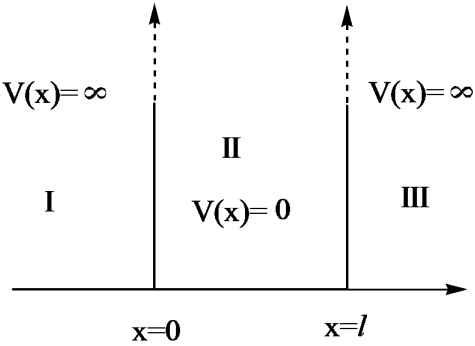
\includegraphics[scale=0.6]{fig/lzhx/微信图片_20211025092646.png}
\end{center}

我们给定一维势箱,粒子的势能$V(x)$为分段函数:
\[V(x)=\left\{
\begin{array}{rl}
+\infty & x<0\\
0 & 0 \leq x \leq l\\
+\infty & x>l
\end{array} \right.\]

由薛定谔方程,我们可以变形得到:
\[-\frac{\hbar^2}{2m}\nabla^2\varPsi+V\varPsi=E\varPsi \quad \Rightarrow \quad \varPsi=\frac{\hbar^2}{2m(V-E)}\nabla^2\varPsi\]

显然,我们能得到:
\[\lim_{V \rightarrow +\infty}\varPsi=0\]

因此,粒子波函数只可能出现在$x \in [0,l]$的范围内,且为保证连续性,波函数还需满足满足下列边界条件$\varPsi(0)=0, \ \varPsi(l)=0$,在这种意义下势箱波函数可以看成是一种驻波:
\[\varPsi(0)=C_1\sin \ 0+C_2\cos \ 0=0 \Rightarrow C_2=0\]
\[\varPsi(l)=C_1\sin(\frac{\sqrt{2mE}}{\hbar}l)=0 \quad \Rightarrow \quad E=\frac{n^2 \pi^2 \hbar^2}{2ml^2}=\frac{n^2 h^2}{8ml^2} \quad (n\in\mathbb{N}_+)\]
利用边界条件$\varPsi(l)=0$,我们得到一维势箱能量量子化。

最后利用归一化得到一维势箱波函数及能量表达式:
\[\int_0^l\varPsi^*\varPsi\dd{x}=C_1^2\int_0^l \sin^2\left (\frac{n \pi}{l}x \right )\dd{x}=\frac{C_1^2}{2}\int_0^l\left ( 1- \cos\left (\frac{2n \pi}{l}x \right ) \right )\dd{x}=\frac{C_1^2l}{2}=1 \quad \Rightarrow \quad C_1=\sqrt{\frac{2}{l}}\]
\[\varPsi_n=\sqrt{\frac{2}{l}}\sin\left (\frac{n \pi}{l}x \right ), \quad E_n=\frac{n^2 h^2}{8ml^2} \quad (n\in\mathbb{N}_+)\]

\begin{center}
    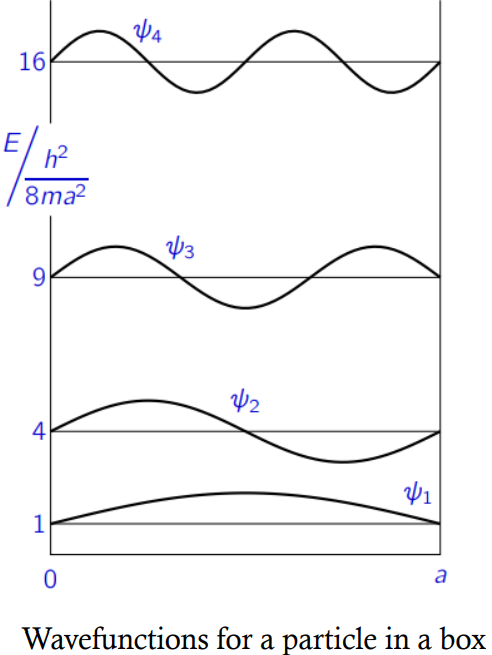
\includegraphics[scale=0.6]{fig/lzhx/微信图片_20211025150139.png}
\end{center}

\subsection{三维势箱}
三维势箱在利用分离变量的方法可以看成三个一维势箱的乘积,这里我们简单介绍一下分离变量法在势箱中的应用,假设三维势箱三个坐标相互独立,则三维势箱波函数可以写成:
\[\varPsi(x,y,z):=X(x)Y(y)Z(z)\]
此时薛定谔方程可以展开为:
\[-\frac{\hbar^2}{2m}\nabla^2\varPsi=-\frac{\hbar^2}{2m}\left (YZ\frac{\partial^2X}{\partial x^2}+XZ\frac{\partial^2Y}{\partial y^2}+XY\frac{\partial^2Z}{\partial z^2} \right )=EXYZ\]

显然,除了平凡解$\psi=0$外,我们可以认为解出的波函数仅在有限个点上取值为零,不考虑这些奇异点,我们将方程两边同时除以$XYZ$:
\[-\frac{\hbar^2}{2m}\left (\frac{1}{X}\frac{\partial^2X}{\partial x^2}+\frac{1}{Y}\frac{\partial{d}^2Y}{\partial y^2}+\frac{1}{Z}\frac{\partial^2Z}{\partial z^2} \right )=E\]

同样的,我们定义:
\[E:=E_x+E_y+E_z\]

因此,我们可以将上述三维势箱薛定谔方程方程写成三个一维势箱薛定谔方程:
\[-\frac{\hbar^2}{2m}\frac{\mathrm{d}^2X}{\mathrm{d}x^2}=E_xX, \qquad -\frac{\hbar^2}{2m}\frac{\mathrm{d}^2Y}{\mathrm{d}y^2}=E_yY, \qquad -\frac{\hbar^2}{2m}\frac{\mathrm{d}^2Z}{\mathrm{d}z^2}=E_zZ\]

求解并合并得到三维势箱的波函数及能量:
\[\varPsi=\sqrt{\frac{8}{abc}}\sin\left (\frac{n_x \pi}{l}x \right )\sin\left (\frac{n_y \pi}{l}y \right )\sin\left (\frac{n_z \pi}{l}z \right ), \quad E_{x,n}=\frac{h^2}{8m} \left (\frac{n_x^2}{a^2}+\frac{n_y^2}{b^2}+\frac{n_z^2}{c^2} \right ) \quad (n_x,n_y,n_z \in \mathbb{N}_+)\]

\section{振动量子化——谐振子}
对于一个处于振动势的双体系统,我们可以把哈密顿量构造成:
\[\hat{H}=-\frac{\hbar^2}{2m_1}\nabla^2_1-\frac{\hbar^2}{2m_2}\nabla^2_2+V\]
考虑质心系:
\[\bm{R}=\frac{m_1\bm{r}_1+m_2\bm{r}_2}{m_1+m_2}, \quad \bm{r}=\bm{r}_1-\bm{r}_2 \quad \Rightarrow \quad \bm{r}_1=\bm{R}+\frac{m_2}{m_1+m_2}\bm{r}, \quad \bm{r}_2=\bm{R}-\frac{m_1}{m_1+m_2}\bm{r}\]
可以吧哈密顿重构成(你可以在经典的情况下推出质心系的哈密顿然后用算符换回来):
\[\hat{H}=-\frac{\hbar^2}{2M}\nabla^2_{\bm{R}}-\frac{\hbar^2}{2\mu}\nabla^2_{\bm{r}}+V(\bm{r}), \quad M=m_1+m_2, \quad \mu=\frac{m_1m_2}{m_1+m_2}\]
可以看出质心的运动形式为自由粒子且与两质点的相对运动解耦,且势能仅取决于两质点之间的相对位置,因此我们我们只需要考虑沿着质点之间相对运动方向$\mathbf{e}_{\bm{r}}$的薛定谔方程:
\[\left(-\frac{\hbar^2}{2\mu}\dv[2]{x}+\frac{1}{2}\mu\omega^2x^2\right)\psi(x)=E\psi(x)\]
方便求解该方程,引入无量纲化:
\[x_0=\sqrt{\frac{\hbar}{\mu\omega}}, \quad \xi=\frac{x}{x_0}, \quad \lambda=\frac{2E}{\hbar\omega}\]
此时谐振子薛定谔方程可以被写成:
\[\dv[2]{\psi}{\xi}+(\lambda-\xi^2)\psi=0\]
当$\xi\to\infty$,观察到(我也不知道他们是怎么观察到的,注意力惊人)其渐进行为$\psi\sim\exp(\pm\xi^2/2)$,为了保证无穷远处收敛性只能取负,因此假设谐振子波函数具有以下形式:
\[\psi(\xi)=u(\xi)e^{-\xi^2/2}\]
带入原方程并化简:
\[\dv[2]{u}{\xi}-2\xi\dv{u}{\xi}+(\lambda-1)u=0\]
这种 ODE 就不要想着怎么巧解了,直接走流程(正)级数展开(反正这里是纯实数方程,没必要展开到洛朗级数)并求解系数方程得到递推关系式(这我就没必要展示了吧,太占用空间了,自己推去):
\[u(\xi)=\sum_{\nu=0}a_{\nu}\xi^{\nu} \quad \Rightarrow \quad a_{\nu+2}=\frac{2\nu+1-\lambda}{(\nu+1)(\nu+2)}a_{\nu}\]
再次渐进分析,并求解通项(我们这里做的只是估计所以不要在意近似得到结果是不是有点不严谨,只需要数量级大致正确就好):
\[\frac{a_{\nu+2}}{a_{\nu}}\sim\frac{2}{\nu} \quad \Rightarrow \quad {a_{\nu}}\sim\frac{C}{(\nu/2)!} \quad \Rightarrow \quad u(\xi)=\sum_{\nu=0}^{\infty}\frac{C}{(\nu/2)!}\xi^{\nu}\sim\sum_{\nu=0}^{\infty}\frac{C}{\nu!}\xi^{2\nu}\sim e^{\xi^2/2}\]
因此,这里的级数不能是一个无穷级数必须要截断,而显然,截断的条件为:
\[2\nu+1-\lambda=0 \quad \Rightarrow \quad E=\frac{\hbar\omega}{2}(2\nu+1)=(\nu+\frac{1}{2})\hbar\omega \quad (\nu \in \mathbb{N})\]
对应的谐振子波函数如下,其中$H_{\nu}(q)$是埃尔米特多项式(Hermite polynomials):
\[\bra{x}\ket{\nu}=\psi_{\nu}(x)=\left(\frac{m\omega}{\pi\hbar}\right)^{1/4}\frac{1}{\sqrt{2^{\nu}\nu!}}H_{\nu}(\xi)e^{-\xi^2/2}, \quad H_{\nu}(\xi)=(-1)^{\nu}e^{\xi^2}\dv[\nu]{\xi}e^{-\xi^2}, \quad (\nu \in \mathbb{N})\]

可以看到纯级数接是累死人的,为了不每次接这种简单体系都类似人以及看到复杂体系就暴毙,我们需要介绍量子力学中的一种常用办法,升降算符法,虽然最后求解波函数可能还是比较复杂,但是在形式上该方法非常普适,可以拓展到非常复杂的体系。首先回到算符形式的谐振子哈密顿量:
\[\hat{H}=\frac{\hat{p}^2}{2\mu}+\frac{1}{2}\mu\omega^2\hat{x}^2\]
定义谐振子的升$(\hat{a}^{\dagger})$降$(\hat{a})$算符如下:
\[\hat{a}=\sqrt{\frac{\mu\omega}{2\hbar}}(\hat{x}+i\frac{1}{\mu\omega}\hat{p}), \quad \hat{a}^+=\sqrt{\frac{\mu\omega}{2\hbar}}(\hat{x}-i\frac{1}{\mu\omega}\hat{p}), \quad [\hat{a},\hat{a}^{\dagger}]=1\]
它们俩与哈密顿量的对易关系$[\hat{a},\hat{H}]=\hbar\omega\hat{a}, \ [\hat{a}^{\dagger},\hat{H}]=\hbar\omega\hat{a}^{\dagger}$。\textcolor{blue}{\textbf{一般当算符与哈密顿量具有如下$[\hat{a},\hat{H}]\propto\hat{a}$关系时我们可以考虑其为升降算符}}。我们用$\ket{\nu}$来表示谐振子的本征态,把上述两个对易作用到本征态上:
\begin{equation}
\begin{aligned}
[\hat{a},\hat{H}]\ket{\nu}=(\hat{a}\hat{H}-\hat{H}\hat{a})\ket{\nu}=\hbar\omega\hat{a}\ket{\nu} \quad &\Rightarrow \quad \hat{H}\hat{a}\ket{\nu}=(E_n-\hbar\omega)\hat{a}\ket{\nu}=\hat{a}(E_{\nu}-\hbar\omega)\ket{\nu}\\
[\hat{a}^{\dagger},\hat{H}]\ket{\nu}=(\hat{a}^{\dagger}\hat{H}-\hat{H}\hat{a}^{\dagger})\ket{\nu}=-\hbar\omega\hat{a}^{\dagger}\ket{\nu} \quad &\Rightarrow \quad \hat{H}\hat{a}^{\dagger}\ket{\nu}=(E_n+\hbar\omega)\hat{a}^{\dagger}\ket{\nu}=\hat{a}^{\dagger}(E_{\nu}+\hbar\omega)\ket{\nu}
\end{aligned}\label{comma}
\end{equation}
此时我们可以看到当作用量一个升或降算符到系统的本征态上后能量上升或下降了$\hbar\omega$,哈密顿量同样的可以表示为:
\[\hat{H}=\hbar\omega(\hat{a}\hat{a}^{\dagger}-\frac{1}{2})=\hbar\omega(\hat{a}^{\dagger}\hat{a}+\frac{1}{2})\]
而对于任意一个态,根据内积的正定性我们有:
\[\bra{\psi}\hat{a}^{\dagger}\hat{a}\ket{\psi}=|\hat{a}\ket{\psi}|^2\geq0 \quad \bra{\psi}\hat{H}\ket{\psi}=\bra{\psi}\left[\hbar\omega(\hat{a}^{\dagger}\hat{a}+\frac{1}{2})\right]\ket{\psi}\geq\frac{1}{2}\hbar\omega\]
因此态的能量(基态能量)最低只能是$E_0=\hbar\omega/2$,用$\ket{0}$表示基态。而不断把升算符作用到基态上,我们可以发现谐振子本征态的能量满足:
\[E_{\nu}=(\nu+\frac{1}{2})\hbar\omega \quad (\nu \in \mathbb{N})\]

同时,我们还可以利用哈密顿量定义粒子数算符$\hat{N}=\hat{a}^{\dagger}\hat{a}$:
\[\hat{h}\ket{\nu}=\hbar\omega(\hat{a}^{\dagger}\hat{a}+\frac{1}{2})\ket{\nu}=\hbar\omega(\hat{N}+\frac{1}{2})\ket{\nu}=(\nu+\frac{1}{2})\hbar\omega \quad \Rightarrow \quad \hat{N}\ket{\nu}=\hat{a}^{\dagger}\hat{a}\ket{\nu}=\nu\]
观察式\ref{comma}我们发现,升降算符作用到本征态上具有以下效果(升降算符能把当前本征态升降到相邻本征态):
\[\hat{a}\ket{\nu}=f(\nu)\ket{\nu-1}, \quad \hat{a}^{\dagger}\ket{\nu}=g(\nu)\ket{\nu+1}\]
利用粒子数算符以及内积正定性可以计算出:
\[\begin{aligned}
\bra{\nu-1}f(\nu)^2\ket{\nu-1}=\bra{\nu}\hat{a}^{\dagger}\hat{a}\ket{\nu}=\nu \quad &\Rightarrow \quad f(\nu)=\sqrt{\nu}\\
\bra{\nu+1}g(\nu)^2\ket{\nu+1}=\bra{\nu}\hat{a}\hat{a}^{\dagger}\ket{\nu}=\bra{\nu}(\hat{a}^{\dagger}\hat{a}+1)\ket{\nu}=\nu+1 \quad &\Rightarrow \quad g(\nu)=\sqrt{\nu+1}\\
\end{aligned}\]
最终得到体系的升降算符具有以下关系,以及一般本征态的表示方法:
\[\hat{a}\ket{\nu}=\sqrt{\nu}\ket{\nu-1}, \quad \hat{a}^{\dagger}\ket{\nu}=\sqrt{\nu+1}\ket{\nu+1}, \quad \ket{\nu}=\frac{1}{\sqrt{\nu!}}\left(\hat{a}^{\dagger}\right)^{\nu}\ket{0}\]

当然,对一般的振动系统,谐振子近似经常是不够的,这时我们会引入非谐校正,比如引入Morse potential:
\[V(r)=D_e\left[1-e^{-\beta(r-r_e)}\right]^2 \approx D_e\left[\beta^2(r-r_e)^2-\beta^3(r-r_e)^3+o(r-r_e)^3\right]\]

因此,对应于谐振子的力常数$k$有如下关系:
\[k=2\beta^2D_e\]

其能量可以用以下表达式给出:
\[E_\nu=\left(\nu+\frac{1}{2}\right)\hbar\omega-\left(\nu+\frac{1}{2}\right)^2\hbar\omega x_e \qquad x_e=\frac{\hbar\beta^2}{2\mu\omega}=\frac{\hbar\omega}{4D_e}\]

\begin{center}
    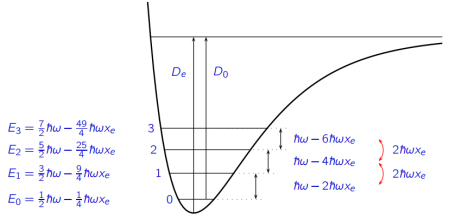
\includegraphics[scale=0.8]{fig/lzhx/微信图片_20211104112141.png}
\end{center}

\section{转动量子化——刚性转子}
在谐振子中我们定义了质心系下两质点的哈密顿量:
\[\hat{H}=-\frac{\hbar^2}{2\mu}\nabla^2_{\bm{r}}+V(\bm{r})\]

在谐振子中我们关心的是两质点沿着两者相对位置方向的运动,而在刚性转动中,我们关心两质点围绕着过质心的某个轴转动,然后通过约化质量的转换,我们相当于构建了一个绕着过原点的某轴旋转的体系,因此体系的势能项$V(\bm{r})=0$,在球坐标下关于$r$的导数项为0:
\[\hat{H}=-\frac{\hbar^2}{2\mu} \left(\frac{1}{r^2\sin\theta}\frac{\partial}{\partial{\theta}}(\sin\theta\frac{\partial}{\partial{\theta}})+\frac{1}{r^2\sin^2 \theta }\frac{\partial^2}{\partial{\phi^2}} \right)\]

带入薛定谔方程并稍作变形:
\[\hat{H}\psi=E\psi \quad \Rightarrow \quad -\hbar^2\left(\frac{1}{r^2\sin\theta}\frac{\partial}{\partial{\theta}}(\sin\theta\frac{\partial}{\partial{\theta}})+\frac{1}{r^2\sin^2 \theta }\frac{\partial^2}{\partial{\phi^2}} \right)\psi=2\mu r^2 E\psi\]

稍微回顾一下经典力学,考虑两个质点$m_1$、$m_2$和轻轴组成的刚性旋转子,两质点间距为$r$,在质心系以及约化质量的引入下系统的转动惯量,角动量以及能量可以被表示为:
\[I=\mu r^2, \quad L=I\omega, \quad E=I\omega^2/2=L^2/2I\]
引入角动量算符$\hat{L}$,我们可以将上述薛定谔方程改写成:
\[\hat{L}^2\psi:=-\hbar^2\left(\frac{1}{r^2\sin\theta}\frac{\partial}{\partial{\theta}}(\sin\theta\frac{\partial}{\partial{\theta}})+\frac{1}{r^2\sin^2 \theta }\frac{\partial^2}{\partial{\phi^2}} \right)\psi=L^2\psi\]

至此我们正式进入了角动量薛定谔方程的求解,这里我们采用升降算符的方式求解,推导过程参考\href{https://zhuanlan.zhihu.com/p/419492575}{cyt大佬的知乎文章}。首先从角动量算符的定义出发,与经典定义一样,角动量算符可以通过位置算符和动量算符的叉乘获得$\hat{\bm{L}}=\hat{\bm{r}}\times\hat{\bm{p}}$,在坐标表象下,显然其有三个分量(显然$\hat{L}_x, \ \hat{L}_y, \ \hat{L}_z, \ \hat{L}^2$都是厄米的,自证不难):
\[\hat{L}_x=\hat{y}\hat{p}_z-\hat{z}\hat{p}_y, \quad \hat{L}_y=\hat{z}\hat{p}_x-\hat{x}\hat{p}_z, \quad \hat{L}_z=\hat{x}\hat{p}_y-\hat{y}\hat{p}_x\]

我们定义升降算符:
\[\hat{L}_+=\hat{L}_x+i\hat{L}_y, \quad \hat{L}_-=\hat{L}_x-i\hat{L}_y\]

这里可以作为一个对易关系式的联系,读者不难自证:
\[[\hat{L}_i,\hat{L}_j]=i\hbar\epsilon_{ijk}\hat{L}_k, \quad [\hat{L}^2,\hat{L}_i]=0, \quad (i,j,k=x,y,z \quad \epsilon_{ijk} \text{ 是\href{https://en.wikipedia.org/wiki/Levi-Civita_symbol}{Levi-Civita符号}})\]

对于升降算符,我们也有以下性质:
\[[\hat{L}_z,\hat{L}_+]=\hbar\hat{L}_+, \quad [\hat{L}_z,\hat{L}_-]=-\hbar\hat{L}_-, \quad [\hat{L}_+,\hat{L}_-]=2\hbar\hat{L}_z, \quad [\hat{L}^2,\hat{L}_+]=[\hat{L}^2,\hat{L}_-]=0\]

由于$\hat{L}^2$与$\hat{L}_z$对易,它们拥有共同的本征态,该本征态分布由两算符对应的量子数$l$与$m_l$确定,记为$\ket{l,m_l}$,我们发现角动量具有$\hbar$的量纲,且由于$\hbar$是量子力学里的最小离散化单位,因此$\hat{L}_z$的本征值一定是$\hbar$的倍数,该整数记为$m_l$,类似的对于$\hat{L}^2$其本征值也应该是$\hbar^2$的倍数,且由于平方的存在这个倍数一定是正的:
\[\hat{L}_z\ket{l,m_l}=m_l\hbar\ket{l,m_l}, \quad \hat{L}^2\ket{l,m_l}=f(l)\hbar^2\ket{l,m_l}\]

对$f(l)$可以更进一步约束其取值范围:
\[\hat{L}^2\ket{l,m_l}-\hat{L}_z^2\ket{l,m_l}=(\hat{L}_x^2+\hat{L}_y^2)\ket{l,m_l}=(f(l)-m_l^2)\hbar^2\ket{l,m_l} \quad \Rightarrow \quad f(l) \geq m_l^2\]

由于升降算符$\hat{L}_{\pm}$与$\hat{L}^2$对易,$\hat{L}_{\pm}$并不改变本征态的$l$部分,而将$\hat{L}_{\pm}$与$\hat{L}_z$的对易子作用到态$\ket{l,m_l}$得到:
\begin{equation}
\begin{aligned}\label{lpm}
\hat{L}_z\hat{L}_+\ket{l,m_l}=\hat{L}_+\hat{L}_z\ket{l,m_l}+[\hat{L}_z,\hat{L}_+]\ket{l,m_l}=m_l\hbar\hat{L}_+\ket{l,m_l}+\hbar\hat{L}_+\ket{l,m_l}=(m_l+1)\hbar\hat{L}_+\ket{l,m_l} \\ \hat{L}_z\hat{L}_-\ket{l,m_l}=\hat{L}_-\hat{L}_z\ket{l,m_l}+[\hat{L}_z,\hat{L}_-]\ket{l,m_l}=m_l\hbar\hat{L}_-\ket{l,m_l}-\hbar\hat{L}_-\ket{l,m_l}=(m_l-1)\hbar\hat{L}_-\ket{l,m_l}
\end{aligned}    
\end{equation}
可以发现,$\hat{L}_{\pm}$作用到态$\ket{l,m_l}$后以$\pm\hbar$的幅度改变了$\hat{L}_z$的本征值,而由于$m_l^2 \leq f(l)$,这说明存在一个最大的$m_l=m_{l,\rm{max}}$满足:
\[\hat{L}_+\ket{l,m_{l,\rm{max}}}=0\]
此时再作用个降算符上去也会得到0:
\begin{equation}
\begin{aligned}\label{l2pm}
\hat{L}_-\hat{L}_+\ket{l,m_{l,\rm{max}}}&=(\hat{L}_x-i\hat{L}_y)(\hat{L}_x+i\hat{L}_y)\ket{l,m_{l,\rm{max}}}=(\hat{L}_x^2+\hat{L}_y^2+i[\hat{L}_x,\hat{L}_y])\ket{l,m_{l,\rm{max}}}\\
&=(\hat{L}^2-\hat{L}_z^2-\hbar\hat{L}_z)\ket{l,m_{l,\rm{max}}}=[f(l)-m_{l,\rm{max}}^2-m_{l,\rm{max}}]\hbar^2\ket{l,m_{l,\rm{max}}}=0
\end{aligned}
\end{equation}
令$l=m_{l,\rm{max}}$,得到$\hat{L}^2$的本征值:
\[\hat{L}^2\ket{l,m_l}=l(l+1)\hbar^2\ket{l,m_l}\]
进而可以知道$m_l$可以取值$-l,-l+1,\cdots,0,\cdots,l-1,l$。

接下来看升降算符的递推形式,从式\ref{lpm}出发,可以看出当升降算符作用在态$\ket{l,m_l}$具有以下形式:
\[\hat{L}_+\ket{l,m_l}=\alpha_+(l,m_l)\hbar\ket{l,m_l+1}, \quad \hat{L}_-\ket{l,m_l}=\alpha_-(l,m_l)\hbar\ket{l,m_l-1}\]
利用式\ref{l2pm}中的结论,我们知道:
\[\hat{L}_-\hat{L}_+\ket{l,m_l}=[l(l+1)-m_l(m_l+1)]\hbar^2\ket{l,m_l}=\alpha_+(l,m_l)\alpha_-(l,m_l+1)\hbar^2\ket{l,m_l}\]
同时:
\[\bra{l,m_l}\hat{L}_-\ket{l,m_l+1}^*=\bra{l,m_l+1}\hat{L}_+\ket{l,m_l} \quad \Rightarrow \quad \alpha_-(l,m_l+1)^*=\alpha_+(l,m_l)\]
整合以上两式可以知道:
\[\hat{L}_+\ket{l,m_l}=\sqrt{l(l+1)-m_l(m_l+1)}\hbar\ket{l,m_l+1}, \quad \hat{L}_-\ket{l,m_l}=\sqrt{l(l+1)-m_l(m_l-1)}\hbar\ket{l,m_l-1}\]

角动量的本征态是球谐函数$\bra{\bm{r}}\ket{l,m_l}=Y_{l,m_l}(\theta,\phi)$,具体的内容可以参考教科书或者\href{https://zhuanlan.zhihu.com/p/419492575}{cyt大佬的知乎文章}。

\begin{center}
    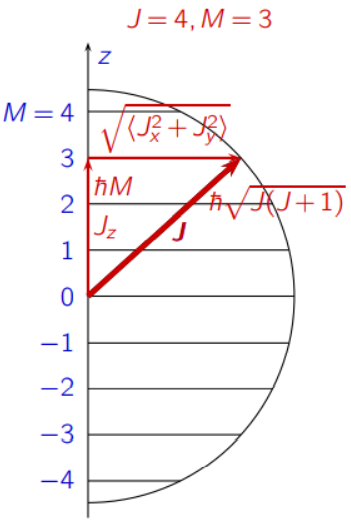
\includegraphics[scale=0.55]{fig/lzhx/微信图片_20211026130340.png}
\end{center}

\section{氢原子}
\subsection{氢原子薛定谔方程求解}
想看自己看第\ref{hydrgen}章。

\subsection{实、复轨道?}
举个例子,求解氢原子薛定谔方程我们能得到$n=2$,$l=1$,$m=-1,0,1$三个轨道波函数的表达式:
\[2p_0=N_{2p}ze^{-\frac{r}{2}}, \quad 2p_1=-N_{2p}\frac{\sqrt{2}}{2}(x+iy)e^{-\frac{r}{2}}, \quad 2p_{-1}=N_{2p}\frac{\sqrt{2}}{2}(x-iy)e^{-\frac{r}{2}}\]

这些轨道与我们所熟知的$2p_x,2p_y,2p_z$有如下关系:
\[2p_z=2p_0=N_{2p}ze^{-\frac{r}{2}} \quad 2p_x=\frac{\sqrt{2}}{2}(2p_{-1}-2p_1)=N_{2p}xe^{-\frac{r}{2}} \quad 2p_y=\frac{\sqrt{2}i}{2}(2p_{-1}+2p_1)=N_{2p}ye^{-\frac{r}{2}}\]

由于能量简并,这几个轨道的线性组合得到的任意波函数都是哈密顿量的本征函数,如果轨道能量不简并的话,轨道线性组合的结果将并不会是哈密顿量的本征函数,其对算符作用后得到的也不是本征值而是期望值。

\section{电子自旋}
非相对论量子力学体系下,电子自旋被认为是电子的内禀性质,这里就不介绍历史了,总而言之,发现自旋与角动量具有相同的量纲,于是强行跟轨道角动量类比得到:
\[\hat{S}^2\ket{s,m_s}=s(s+1)\hbar^2\ket{s,m_s}, \quad \hat{S}_z\ket{s,m_s}=m_s\hbar\ket{s,m_s}\]
\[[\hat{S}^2,\hat{S}_i]=0, \quad [\hat{S}_i,\hat{S}_j]=i\hbar\epsilon_{ijk}\hat{S}_k, \quad (i,j,k=x,y,z)\]

我们定义升降算符:
\[\hat{S}_+=\hat{S}_x+i\hat{S}_y, \quad \hat{S}_-=\hat{S}_x-i\hat{S}_y\]
对于升降算符,我们也有以下性质:
\[[\hat{S}_z,\hat{S}_+]=\hbar\hat{S}_+, \quad [\hat{S}_z,\hat{S}_-]=-\hbar\hat{S}_-, \quad [\hat{S}_+,\hat{S}_-]=2\hbar\hat{S}_z, \quad [\hat{S}^2,\hat{S}_+]=[\hat{S}^2,\hat{S}_-]=0\]

实验上观测到的电子只有两种自旋,即$s=1/2, \ m_s=\pm1/2$,对应的电子自旋态记为$\ket{\uparrow},\ket{\downarrow}$,这两者是$\hat{S}^2,\hat{S}_z$的本征态,在$\ket{\uparrow},\ket{\downarrow}$张成的空间下,$\hat{S}_z$和$\hat{S}^2$可以表示成如下形式:
\[\hat{S}_z=\frac{\hbar}{2}\begin{pmatrix} 1 & 0 \\ 0 & -1 \end{pmatrix}, \quad \hat{S}^2=\frac{3}{4}\hbar^2\begin{pmatrix} 1 & 0 \\ 0 & 1 \end{pmatrix}\]

根据升降算符的性质$\hat{S}_{\pm}\ket{s,m_s}=\sqrt{s(s+1)-m_s(m_s\pm1)}\hbar\ket{s,m_s\pm1}$可以得出升降算符的矩阵表示:
\[\hat{S}_+=\hbar\begin{pmatrix} 0 & 1 \\ 0 & 0 \end{pmatrix}, \quad \hat{S}_-=\hbar\begin{pmatrix} 0 & 0\\ 1 & 0 \end{pmatrix}\]
进而能反推出$\hat{S}_x,\hat{S}_y$:
\[\hat{S}_x=\frac{1}{2}(\hat{S}_++\hat{S}_-)=\frac{\hbar}{2}\begin{pmatrix} 0 & 1 \\ 1 & 0 \end{pmatrix}, \quad \hat{S}_y=\frac{1}{2i}(\hat{S}_+-\hat{S}_-)=\frac{\hbar}{2}\begin{pmatrix} 0 & -i \\ i & 0 \end{pmatrix}\]

\begin{center}
    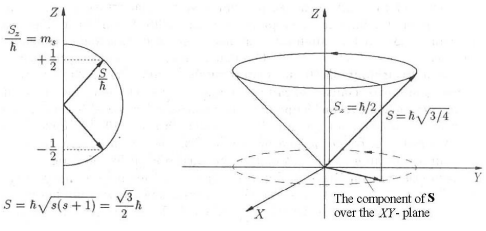
\includegraphics[scale=0.7]{fig/lzhx/微信图片_20211028113518}
\end{center}

定义泡利矩阵(Pauli Matrices)引入归一化:
\[\hat{\bm{S}}=(\hat{S}_x,\hat{S}_y,\hat{S}_z)=\frac{\hbar}{2}\hat{\bm{\sigma}}=\frac{\hbar}{2}(\hat{\sigma}_x,\hat{\sigma}_y,\hat{\sigma}_z)\]
泡利矩阵具有如下性质:
\[[\hat{\sigma}_i,\hat{\sigma}_j]=2i\epsilon_{ijk}\hat{\sigma}_k, \quad \hat{\sigma}_i^2=\hat{\sigma}_i^{\dagger}\hat{\sigma}_i=\mathbf{I}, \quad \Tr\hat{\sigma}_i=0, \quad (i,j,k=x,y,z)\]

\subsection{SU(2)和SO(3)}
SU(2) 群是一个矩阵群,群元素为$2\times2$的幺正矩阵,而且矩阵的行列式为1。如果将 SU(2) 群元素写做$e^{iA}$,那么因为 $e^{iA}(e^{-iA})^\dagger=e^{iA}e^{-iA^\dagger}=I \ \Rightarrow \ A=A^\dagger$,也就是$A$是Hermite矩阵。又因为$\det(e^{iA})=e^{i\Tr A}=1$,所以$\Tr A=0$。任意一个零迹二阶Hermite矩阵都可以用三个泡利矩阵的线性组合给出,因此 SU(2) 的基本元素都可以用泡利矩阵表示成$e^{i\frac{\theta}{2}\bm{\sigma}\cdot\bm{n}}, \ \bm{n}\in\mathbb{R}^3, \ |n|=1$。由于这里有四个变量一个约束条件,指数映射将李代数映射到李群,因此 SU(2) 是一个三阶连续群。所以泡利矩阵是 SU(2) 群的李代数 su(2) 的一组完备基。

SO(3) 群是所有行列式为1的$3\times3$的正交矩阵构成的集合。用指数形式表示一个正交矩阵为$R=e^A$ .根据定义,有$R^TR=e^{A^T}e^A=I$ .所以就有$A^T=-A$ ,意味着$A$是反对称矩阵。另外,$\det R=e^{\mathrm{Tr}A}=1$ .所以$\Tr A=0$ .值得指出的是,反对称实矩阵的迹一定是零。所以 SO(3) 群的李代数 so(3) 是所有三阶反对称实矩阵构成的集合。任意一个三阶反对称实矩阵都可以写作
\[A=\begin{pmatrix}0&-a&b\\a&0&-c\\-b&c&0\end{pmatrix}\]
因此, SO(3)群也是只有三个自由度,是一个三阶连续群。

\begin{definition}[群同态]
给定两个群$(G,\ast),(H,\cdot)$和映射$h:(G,*)\to(H,\cdot)$, 满足:
\[\forall \, u,v \in G, \ h(u*v)=h(u)\cdot h(v)\]
则称映射$h$为群同态。
\end{definition}

同态映射保持了群的结合律,同时也需要注意,群同态并不保证其是单、满还是双的,下面我们将证明存在一个从 SU(2) 到 SO(3) 的群同态(略去结合律的验证,这很显然),然后说明这是一个2/1的满同态。

\[
\begin{tikzcd}[row sep=1.5cm, column sep=1.5cm]
x\in\mathbb{R}^3 \arrow[r, "y=Rx"] \arrow[d, "\exp(i\theta\bm{x}\cdot\bm{\sigma}/2)"'] 
    & y\in\mathbb{R}^3 \arrow[d, "\exp(i\theta\bm{y}\cdot\bm{\sigma}/2)"] \\
X\in\text{SU(2)} \arrow[r, "UXU^\dagger"] 
    & Y\in\text{SU(2)}
\end{tikzcd}
\]

构造以上的映射关系,从$\mathbb{R}^3$中取出一个元素$x$一一映射到 SU(2) 中的$X$,然后定义一个关于 SU(2) 中的元素$U$的映射把$X$映射到$Y$,最后再利用与第一步一样的映射取出$\mathbb{R}^3$中的另外一个元素$y$,只需要说明对于每一个 SU(2) 中的元素$U$都能找到一个 SO(3) 中的元素$R$与之对应。计算$UXU^\dagger$:
\[UXU^\dagger=\sum_{i=1}^{3}x_ie^{i\frac{\theta}{2}\bm{\sigma}\cdot\bm{n}}\sigma_ie^{-i\frac{\theta}{2}\bm{\sigma}\cdot\bm{n}}:=\sum_{i=1}^{3}x_if_i(\theta)\]
需要求解$f_i(\theta)$,先导一发(会用到$[\bm{\sigma}\cdot\bm{n},\sigma_i]=-[\sigma_i,\sigma_j]n_j=-2i\epsilon_{ijk}n_j\sigma_k$,这里用了爱因斯坦求和约定):
\[f_i^{\prime}(\theta)=\frac{i}{2}e^{i\frac{\theta}{2}\bm{\sigma}\cdot\bm{n}}[\bm{\sigma}\cdot\bm{n},\sigma_i]e^{-i\frac{\theta}{2}\bm{\sigma}\cdot\bm{n}}=\sum_{j}\epsilon_{ijk}n_j\frac{i}{2}e^{i\frac{\theta}{2}\bm{\sigma}\cdot\bm{n}}\sigma_ke^{-i\frac{\theta}{2}\bm{\sigma}\cdot\bm{n}}=\sum_{j}\epsilon_{ijk}n_jf_k(\theta)\]
写成矩阵形式$\mathbf{F}'=\mathbf{A}\mathbf{F}$(又是一个复习数学的好时候):
\[\mathbf{F}'=\begin{pmatrix}f_1^{\prime}(\theta)\\f_2^{\prime}(\theta)\\f_3^{\prime}(\theta)\end{pmatrix}=\begin{pmatrix}0&-n_3&n_2\\n_3&0&-n_1\\-n_2&n_1&0\end{pmatrix}\begin{pmatrix}f_1(\theta)\\f_2(\theta)\\f_3(\theta)\end{pmatrix}=\mathbf{A}\mathbf{F}\]
除了直接对角化解方程外这里介绍一些特殊性质,由于矩阵$\mathbf{A}$是反对称的,这意味着$\mathbf{A}\mathbf{F}=\mathbf{n}\times\mathbf{F}$,这表明这个是一个绕着$\mathbf{n}$轴的旋转方程,其解为$\mathbf{F}(\theta)=e^{\theta\mathbf{A}}\mathbf{F}(0)=R\bm{\sigma}$,显然这里$R$是上文提到的 SO(3) 的元素。

整理一下上述计算:
\[Y=\sum_{i=1}^3y_i\sigma_i=\sum_{i=1}^{3}x_if_i(\theta)=\sum_{i=1}^{3}x_i\sum_{j=1}^{3}R_{ij}\sigma_j \quad \Rightarrow \quad \mathbf{y}=R\mathbf{x}\]

这需要说明对于每一个 SU(2) 中的元素$U$都能找到一个 SO(3) 中的元素$R$与之对应,即证明了从 SU(2) 到 SO(3) 的同态是满的:
\[U(\theta)=e^{i\frac{\theta}{2}\bm{\sigma}\cdot\bm{n}} \to R(\theta)=e^{\theta\mathbf{A}}, \quad \text{SU(2)} \mapsto \text{SO(3)}\]
保结合律是显然的。值得注意的是$U(\theta)$与$U(\theta+2\pi)$都对应同一个$R(\theta)$,但是两者并不相等,这一数学事实直接导致了自旋$1/2$系统在旋转下的非经典行为:波函数在空间旋转$2\pi$后改变符号,需要旋转$4\pi$才能复原。这是量子力学区别于经典物理的一个最深刻、最典型的特征。


\section{单核多电子体系}
\subsection{波恩-奥本海默(Born-Oppenheimer)近似}
理论上对于一个微观体系,只要我们确定了粒子组成及其相互作用,我们就能写出该体系的哈密顿量,利用基本假设薛定谔方程去求解体系的波函数。但是实际上你解个氢原子都解得要死要活的了,甚至氢分子你都不能给出解析解。那么引入一些近似在不降低太多准确度的前提下大幅提高计算的速度就显得尤为重要。这里我们将介绍一个最普遍的近似——波恩-奥本海默(BO)近似。

哈密顿量可以写成动能部分和势能部分,那么我们还能继续拆下去吗,该怎么拆呢?一个自然而然的想法就是我们能不能把核的运动和电子的运动分离开呢?于是我们就假设核跟电子的运动无关,进而可以将动能项拆成核动能部分和电子动能部分:
\[\hat{H}=\hat{T_n}+\hat{T_e}+\hat{V}_n+\hat{V}_e=\hat{T_n}+\hat{H_e}=-\sum_i\frac{\hbar^2}{2m_{n,i}}\nabla^2_{n,i}-\sum_j\frac{\hbar^2}{2m_e}\nabla^2_{e,j}+\sum_{ni,ej}V_{ni,ej}+\sum_{ei,ej}V_{ei,ej}\]

由于核的运动与电子的运动解耦,我们假设电子的波函数$\psi(\bm{Q},\bm{q})$和核的波函数$\varphi(\bm{Q})$可以分离,于是波函数可以写成如下形式,其中$\bm{Q}$为核坐标,$\bm{q}$为电子坐标:
\[\varPsi(\bm{Q},\bm{q})=\psi(\bm{Q},\bm{q})\varphi(\bm{Q})\]

由于解耦,对电子部分的薛定谔方程来说核坐标$\bm{Q}$被视为参数引入,电子感受到核势能$\hat{V}_n$退化为常数。这就意味着,反复求解不同核坐标微小变化下的电子薛定谔方程可以获得电子能量$U(\bm{Q})$关于核坐标$\bm{Q}$函数,成为势能面(PES)。由于这种将电子波函数重新计算为无穷小变化的核几何形状的函数的过程让人想起绝热定理的条件,因此这种获得 PES 的方式通常称为绝热近似,而 PES 本身称为绝热面。

正如BO近似的另一个名字定核近似,简单理解,电子相对于核运动太快,波恩-奥本海默近似就是认为核不动,当然这是不对的,\textcolor{blue}{\textbf{BO近似认为的是电子相较于原子核运动很快所以认为核坐标变化后电子总能在瞬间达到新的平衡}},所以有$\nabla^2_n\psi(\bm{Q},\bm{q}) \approx 0, \ \nabla_n\psi(\bm{Q},\bm{q}) \approx 0$。

将哈密顿量作用在波函数上,先看核动能部分:
\[\begin{aligned}
\hat{T_n}\varPsi(\bm{Q},\bm{q})&=-\sum_i\frac{\hbar^2}{2m_{n,i}}\left (\nabla^2_{n,i}\psi(\bm{Q},\bm{q}) \cdot \varphi(\bm{Q})+2\nabla_{n,i}\psi(\bm{Q},\bm{q}) \cdot \nabla_{n,i}\varphi(\bm{Q})+ \psi(\bm{Q},\bm{q}) \cdot \nabla^2_{n,i}\varphi(\bm{Q})  \right )\\ 
&\approx -\sum_i\frac{\hbar^2}{2m_{n,i}}\psi(\bm{Q},\bm{q}) \cdot \nabla^2_{n,i}\varphi(\bm{Q})=-\psi(\bm{Q},\bm{q})\sum_i\frac{\hbar^2}{2m_{n,i}}\nabla^2_{n,i}\varphi(\bm{Q})
\end{aligned}\]

考虑电子动能部分:
\[\hat{T_e}\varPsi(\bm{Q},\bm{q})=-\varphi(\bm{Q})\sum_j\frac{\hbar^2}{2m_e}\nabla^2_{e,j}\psi(\bm{Q},\bm{q})\]

合并整个哈密顿量,可以将薛定谔方程改写成如下形式:
\[\hat{H}\varPsi(\bm{Q},\bm{q})=-\psi(\bm{Q},\bm{q})\sum_i\frac{\hbar^2}{2m_{n,i}}\nabla^2_{n,i}\varphi(\bm{Q})-\varphi(\bm{Q})\sum_j\frac{\hbar^2}{2m_e}\nabla^2_{e,j}\psi(\bm{Q},\bm{q})+\sum_{i,j}V_{i,j}\psi(\bm{Q},\bm{q})\varphi(\bm{Q})=E\psi(\bm{Q},\bm{q})\varphi(\bm{Q})\]
利用分离变量获得电子薛定谔方程:
\[-\sum_j\frac{\hbar^2}{2m_e}\nabla^2_{e,j}\psi(\bm{Q},\bm{q})+\sum_{i,j}V_{i,j}\psi(\bm{Q},\bm{q})=U(\bm{Q})\psi(\bm{Q},\bm{q})\]
与核运动方程:
\[-\sum_i\frac{\hbar^2}{2m_{n,i}}\nabla^2_{n,i}\varphi(\bm{Q})=[E-U(\bm{Q})]\varphi(\bm{Q})\]

电子结构所关心的是电子薛定谔方程,解出给定核构型下的电子分布,而动力学关心的是核薛定谔方程,认为给定核构型下的电子结构是已知的。一个有意思的事是:我们求解氢原子的波函数时用的是只含电子项的薛定谔方程,但是我们依然说这个是精确解,这是为什么呢?\textcolor{blue}{\textbf{因为波恩-奥本海默近似本质上是假定变量可分离,因此对实际上确实可分离的体系这就不是一种近似}}。BO近似是必要的,毕竟三体以上的系统我们没法精确求解。

\subsection{平均场(Mean field)近似}
至此,在BO近似后,我们开始接触多电子体系,需要注意的是现在我们其实还是不能直接处理这样的多电子体系,主要的原因是电子-电子相互作用我们处理不了(本质上还是三体以上的系统没法精确求解),所以我们需要考虑进一步近似把多电子体系近似成我们能处理的单电子体系。

考虑一个多电子多核系统,其电子哈密顿量可以表示成:
\[\hat{H}=-\sum_{i}\frac{\hbar^2}{2m_i}\nabla^2_i+\sum_{i,j}\frac{q_iq_j}{4 \pi \varepsilon_0 r_{ij}}-\sum_i\frac{q_iq_n}{4 \pi \varepsilon_0 r_{i}}\]

在平均场近似下,把其他电子对某电子的双体算符$(\hat{V}_{ij})$平均成其他电子对该电子产生的势场$(\hat{V}_{i})$,此时体系哈密顿算符可以被拆分成单个粒子的哈密顿算符之和:
\[\hat{H}=\sum_{i}\hat{H}_{i} \quad \text{where} \quad \hat{H}_i=-\frac{\hbar^2}{2m_i}\nabla^2_i+V_{n,i}+V_{e,i}, \quad V_{e,i}=\frac{1}{4\pi\varepsilon_0}\sum_{j\neq i}\int\frac{|\psi_j(\bm{r})|^2}{|\bm{r}_j-\bm{r}_i|}\dd{\bm{r}_j}\]

同理,电子波函数也可以近似成各个单电子波函数的乘积$\varPsi=\varPsi_1(\bm{q}_1)\varPsi_2(\bm{q}_2)\cdots$(这里先对波函数这样的拆分方法正确性按下不表),此时系统的总薛定谔方程可以被拆分成一系列的单体薛定谔方程:
\[\hat{H}_i\ket{\psi_i}=\left( -\frac{\hbar^2}{2m_i}\nabla^2_i+\hat{V}_i \right)\ket{\psi_i}=\varepsilon_i\ket{\psi_i}\]
但此时哈密顿包含了波函数,因为你需要用波函数来计算电子密度从而构建平均场,即你要解的方程是一个$\hat{H}(\psi)\ket{\psi}=E\ket{\psi}$形式的本征值问题,你当然不能直接对角化哈密顿,此时需要迭代来收敛最终得到波函数,这种方法称为自洽场(Self-Consistent Field, SCF)。
\subsection{粒子全同性与泡利不相容原理}
全同性应该是微观粒子与宏观物体最不同的地方之一。

简单来说,对两个宏观物体A、B,除了速度、位置外,我们还有大小、颜色之类的特征作为区分物体A、B,这也即表面在经典物理框架下,并没有全同性这一说法。但对于微观粒子A、B,我们似乎只有速度和位置这类无法区分粒子的可观测量。

\textbf{而对微观粒子,你可以通过测量获得粒子的一个一个一个物理量,但是会发现你测量你舌头上的电子跟野兽先辈林檎上的电子也能测出一样的物理量,即使把你舌头上的电子和野兽先辈林檎上的电子调换一下,你的舌头和野兽先辈的林檎都还是安然无恙的(保持不变),这也就是微观粒子的全同性。}

接下来,我们的表述将在全同性这一微观粒子基本性质下展开。

首先定义对换算符$\hat{P}_{ij}$:
\[\hat{P}_{ij}\varPsi(\cdots,i,\cdots,j,\cdots)=\varPsi(\cdots,j,\cdots,i,\cdots)\]

基于全同性,就一个多粒子体系而言,我们调换一对同类型的粒子,显然其分布概率(经典物理量)并不会被改变(有经典对应的物理量在埃伦费斯特定理(Ehrenfest's theorem)的保证下符合经典物理的行为):
\[\begin{aligned}
|\varPsi(\cdots,i,\cdots,j,\cdots)|^2&=|\varPsi(\cdots,j,\cdots,i,\cdots)|^2 \\ 
\varPsi(\cdots,i,\cdots,j,\cdots)&=\pm\varPsi(\cdots,j,\cdots,i,\cdots)
\end{aligned}\]

依据上述描述,对换算符和哈密顿算符必然是对易的:
\[\qty[\hat{P}_{ij},\hat{H}]=0\]

对应,上述两种波函数行为,我们定义两类粒子——玻色子和费米子:
\[
    \begin{array}{lll}
        \text{Boson} & \varPsi(\cdots,i,\cdots,j,\cdots)=\varPsi(\cdots,j,\cdots,i,\cdots) & \text{symmetric} \\
        \text{Fermion} & \varPsi(\cdots,i,\cdots,j,\cdots)=-\varPsi(\cdots,j,\cdots,i,\cdots) & \text{antisymmetric}
    \end{array}
\]

两者在自旋(某种对称性)上有截然不同的特征:玻色子自旋为整数,费米子自旋为半整数。我们来看电子,电子是费米子,所以电子的波函数应该是反对称的。

当然除了一次换电子,我们也可以考虑一次对换多个电子,我们将其记为$\hat{P}_k$,称为置换算符,在线代的行列式部分中已经用到过该算符。利用置换算符我们还可以构造对称算符$\hat{S}$以及反对称算符$\hat{A}$,其中$\tau$为任意n元排列$k$的逆序数,$k$的个数为$n!$:
\[\hat{S}=\frac{1}{\sqrt{n!}}\sum_{k}\hat{P}_{k} \qquad \hat{A}=\frac{1}{\sqrt{n!}}\sum_{k}(-1)^{\tau}\hat{P}_{k}\]

用这两个算符,我们可以构造出多满足泡利不相容原理的玻色子或费米子体系的波函数,以双粒子双能级体系为例,粒子用$1,2$区分,能级用$a,b$区分,\textcolor{blue}{\textbf{注意这里我们引入标号只是为例我们书写方便并不代表微观粒子可以区分}}:
\[\begin{array}{ll}
\text{Boson} & \hat{S}\varPsi_{ab}(1,2)=\frac{1}{\sqrt{2!}}[\varphi_a(1)\varphi_b(2)+\varphi_a(2)\varphi_b(1)]\\
\text{Fermion} & \hat{A}\varPsi_{ab}(1,2)=\frac{1}{\sqrt{2!}}[\varphi_a(1)\varphi_b(2)-\varphi_a(2)\varphi_b(1)] 
\end{array}\]

考虑一件有意思的事情,如果所有粒子处于同一个量子态,玻色子和费米子会有什么样的行为?

我们这里继续使用上述的两个算符构造:
\[\hat{S}\varPsi_{1}(1,2,3 \cdots)=\frac{1}{\sqrt{n!}}\sum_{k}\hat{P}_{k}\varPsi_{1}(1,2,3 \cdots)=\frac{1}{\sqrt{n!}}\cdot n!\prod_{i=1}^n\varphi_1(i)=\sqrt{n!}\prod_{i=1}^n\varphi_1(i)\]
\[\hat{A}\varPsi_{1}(1,2,3 \cdots)=\frac{1}{\sqrt{n!}}\sum_{k}(-1)^{\tau}\hat{P}_{k}\varPsi_{1}(1,2,3 \cdots)=\frac{1}{\sqrt{n!}}\left (\frac{n!}{2}\prod_{i=1}^n\varphi_1(i)-\frac{n!}{2}\prod_{i=1}^n\varphi_1(i) \right )=0\]
这证明了我们为什么只“见过”波色子扎推在一个能级中,而费米子只能孤零零地处于各自不同的能级上。

\subsection{双自旋体系}
如果我们对一个双电子体系进行考察,其自旋可以采用四种状态:$\ket{m_{1s}m_{2s}}=\ket{\uparrow\uparrow},\ket{\uparrow\downarrow},\ket{\downarrow\uparrow},\ket{\downarrow\downarrow}$。我们定义该体系的总自旋角动量z投影算符为:
\[\hat{S}_z=\hat{S}_{1z}+\hat{S}_{2z} \quad \Rightarrow \quad \hat{S}_z\ket{m_{1s}m_{2s}}=\hat{S}_{1z}\ket{m_{1s}m_{2s}}+\hat{S}_{2z}\ket{m_{1s}m_{2s}}=(m_{1s}+m_{2s})\ket{m_{1s}m_{2s}}\]
整理一下结果:
\[M_s=m_{1s}+m_{2s}=\left\{
\begin{array}{ll}
1  & ,\ket{\uparrow\uparrow}\\
0  & ,\ket{\uparrow\downarrow}\text{ and }\ket{\downarrow\uparrow}\\
-1 & ,ß\ket{\downarrow\downarrow}
\end{array}
\right.\]

但我们会发现当$M_s=0$时出现的自旋波函数对称性不满足我们在全同性中给出的要求(不对称的乘上什么都是不对称的),因此我们需要寻找另外的一对满足对称性要求的基底,由于$\ket{\uparrow\downarrow},\ket{\downarrow\uparrow}$对应同一个本征值$M_s=0$,我们可以把这俩线性组合得到的结果也是$M_s=0$对应的本征态。容易想到以下组合
\[\frac{1}{\sqrt{2}}(\ket{\uparrow\downarrow}+\ket{\downarrow\uparrow}), \quad \frac{1}{\sqrt{2}}(\ket{\uparrow\downarrow}-\ket{\downarrow\uparrow})\]

考虑对称性(对换两个粒子的位置看结果),我们可以讲上述四个轨道分为两类:
\[\text{Symmetric: }\ket{\uparrow\uparrow}, \ \ket{\downarrow\downarrow}, \ \frac{1}{\sqrt{2}}(\ket{\uparrow\downarrow}+\ket{\downarrow\uparrow}), \quad \text{Antisymmetric: }\frac{1}{\sqrt{2}}(\ket{\uparrow\downarrow}-\ket{\downarrow\uparrow})\]

类似的,关于这两个电子波函数的空间部分,我们也能构造出对称与反对称的态出来:
\[\text{Symmetric: }\frac{1}{\sqrt{2!}}(\ket{\psi_a(1)\psi_b(2)}+\ket{\psi_a(2)\psi_b(1)}), \quad \text{Antisymmetric: }\frac{1}{\sqrt{2!}}(\ket{\psi_a(1)\psi_b(2)}-\ket{\psi_a(2)\psi_b(1)})\]
将两者组合,为满足电子波函数反对称化的要求,我们只能这么组合:
\[\ket{\Psi_{\rm{singlet}}}=\frac{1}{\sqrt{2!}}(\ket{\psi_a(1)\psi_b(2)}+\ket{\psi_a(2)\psi_b(1)})\otimes\frac{1}{\sqrt{2}}(\ket{\uparrow\downarrow}-\ket{\downarrow\uparrow})\]
\[\ket{\Psi_{\rm{triplet}}}=\frac{1}{\sqrt{2!}}(\ket{\psi_a(1)\psi_b(2)}-\ket{\psi_a(2)\psi_b(1)})\otimes \left\{
    \begin{array}{l}
        \ket{\uparrow\uparrow}\\
        (\ket{\uparrow\downarrow}+\ket{\downarrow\uparrow})/\sqrt{2}\\
        \ket{\downarrow\downarrow}
    \end{array}
\right.
\]
根据简并的数量我们分别命名为单重态和三重态。

这里稍微补充点关于直积$\otimes$和直和$\oplus$的知识,由于电子的自旋在量子力学范畴内是额外假定上去的性质,至少到这里不考虑旋轨耦合的话,认为电子的空间部分和自旋部分就是毫无关联的拼在一起,好比$O$-$xyz$空间是由$xOy$平面上加上$z$-轴拼在一样。此时我们描述一个电子态就不能只用空间部分$\ket{\psi}$或者自旋部分$\ket{m_s}$,我们需要从空间部分选取一个点跟自旋部分选取一个点然后拼起来在新的空间中去描述这个电子态$\ket{\Psi}$,电子态的空间部分跟自旋空间拼起来的操作我们称为直积$\otimes$,包含电子空间部分元素的全空间跟包含电子自旋部分的全空间拼起来的操作我们称为直和$\oplus$:
\[\ket{\Psi}=\ket{\psi}\otimes\ket{m_s}, \quad \mathscr{H}_{\Psi}=\mathscr{H}_{\psi}\oplus\mathscr{H}_{m_s}\]
由于空间自旋部分互不隶属,所以在进行运算的时候分别考虑:
\[\bra{\Phi}\ket{\Psi}=\left(\bra{\phi}\otimes\bra{m_s'}\right)\left(\ket{\psi}\otimes\ket{m_s}\right)=\bra{\phi}\ket{\psi}\bra{m_s'}\ket{m_s}\]
如果考虑哈密顿$\mathscr{H}_{\Psi}$在基$\ket{\Psi}$下的表示的话,实际上就是把$\mathscr{H}_{\psi}$在基$\ket{\psi}$下的矩阵元每个都换成一个$2\times2$的表示自旋部分的矩阵。如果想从$\mathscr{H}_{\Psi}$去掉$\mathscr{H}_{\psi}$或者$\mathscr{H}_{m_s}$的话只需要通过偏迹即可完成。

\subsection{Slater 行列式}
上一小节中我们提到了构造反对称化的全体系电子空间波函数,其方法是使用 Slater 行列式。这里以锂原子为例,数字为电子编号,其 Slater 行列式为,即把所有电子(已知自旋)按反对称化的要求便利所有空间轨道:
\[\varPhi=\frac{1}{\sqrt{n!}}
\left |
\begin{array}{lll}
1s(1)\alpha(1) & 1s(1)\beta(1) & 2s(1)\alpha(1) \\
1s(2)\alpha(2) & 1s(2)\beta(2) & 2s(1)\alpha(2) \\
1s(1)\alpha(3) & 1s(1)\beta(3) & 2s(1)\alpha(3)
\end{array}
\right |
=\frac{1}{\sqrt{n!}}
\left |
\begin{array}{lll}
1s(1) & \overline{1s(1)} & 2s(1) \\
1s(2) & \overline{1s(2)} & 2s(2) \\
1s(3) & \overline{1s(3)} & 2s(3)
\end{array}
\right |
\]
或者,我们可以换一种更简洁的表示方式,利用反对称化算符志杰作用在 Hartree 积(所以轨道乘起来)上:
\[\varPhi=\hat{A}\varPsi_{a_1,a_2,a_3 \cdots}(1,2,3\cdots)=\frac{1}{\sqrt{n!}}\sum_k(-1)^{\tau}\varPsi_{a_k}(k)\]

\subsection{氦原子}
根据上面的讨论,我们可以得到氦原子的$1s2s$激发单重态轨道波函数:
\[\varPsi_{+}=\frac{1}{\sqrt{2!}}[\varphi_a(1)\varphi_b(2)+\varphi_a(2)\varphi_b(1)]\]

久违地考虑一下能量,写出氦原子的电子哈密顿算符(原子单位):
\[\hat{H}=-\sum_{i=1}^2\frac{1}{2}\nabla^2_i-\sum_{i=1}^2\frac{2}{r_{i}}+\frac{1}{r_{12}}\]

定义,单电子体系哈密顿算符为$\hat{h}_i \ (i=1,2)$与对应的能量$\varepsilon$:
\[\hat{h}_i=-\frac{1}{2}\nabla^2_i-\frac{2}{r_{i}}, \quad \bra{\varphi_a}\hat{h}_1\ket{\varphi_a}=\varepsilon \quad \bra{\varphi_b}\hat{h}_2\ket{\varphi_b}=\varepsilon\]
\[E=\bra{\varPsi_{+}}\hat{H}\ket{\varPsi_{+}}=\bra{\varPsi_{+}}\hat{h}_1\ket{\varPsi_{+}}+\bra{\varPsi_{+}}\hat{h}_2\ket{\varPsi_{+}}+\bra{\varPsi_{+}}\frac{1}{r_{12}}\ket{\varPsi_{+}}=2\varepsilon+\bra{\varPsi_{+}}\frac{1}{r_{12}}\ket{\varPsi_{+}}\]
为简化考虑,可以进一步把自旋部分积分掉:
\[\bra{\varPsi_{+}}\frac{1}{r_{12}}\ket{\varPsi_{+}}=\bra{\varphi_{+}}\otimes\bra{\sigma_{\rm{singlet}}}\frac{1}{r_{12}}\ket{\varphi_{+}}\otimes\ket{\sigma_{\rm{singlet}}}=\bra{\varphi_{+}}\frac{1}{r_{12}}\ket{\varphi_{+}}\bra{\sigma_{\rm{singlet}}}\ket{\sigma_{\rm{singlet}}}=\bra{\varphi_{+}}\frac{1}{r_{12}}\ket{\varphi_{+}}\]

具体来看它:
\[\begin{aligned}
\bra{\varphi_{+}}\frac{1}{r_{12}}\ket{\varphi_{+}}&=\frac{1}{2}\int_{\mathbb{R}^{3 \times 2}}[\varphi_a(1)\varphi_b(2)+\varphi_a(2)\varphi_b(1)]^{*}\frac{1}{r_{12}}[\varphi_a(1)\varphi_b(2)+\varphi_a(2)\varphi_b(1)]\dd\tau_1\dd\tau_2 \\ \bra{\varphi_{+}}\frac{1}{r_{12}}\ket{\varphi_{+}}&=\int_{\mathbb{R}^{3 \times 2}} \left( [\varphi_a(1)\varphi_b(2)]^{*}\frac{1}{r_{12}}[\varphi_a(1)\varphi_b(2)]+[\varphi_a(1)\varphi_b(2)]^{*}\frac{1}{r_{12}}[\varphi_a(2)\varphi_b(1)] \right)\dd\tau_1\dd\tau_2
\end{aligned}\]

定义库伦积分$J$(与经典物理中的定义相符)和交换积分$K$(没有经典对应,不知道哪来的):
\[J=\int_{\mathbb{R}^{3 \times 2}}[\varphi_a(1)\varphi_b(2)]^{*}\frac{1}{r_{12}}[\varphi_a(1)\varphi_b(2)]\dd\tau_1\dd\tau_2, \quad K=\int_{\mathbb{R}^{3 \times 2}}[\varphi_a(1)\varphi_b(2)]^{*}\frac{1}{r_{12}}[\varphi_a(2)\varphi_b(1)]\dd\tau_1\dd\tau_2\]

最后,我们得到:
\[\bra{\varPsi_{+}}\frac{1}{r_{12}}\ket{\varPsi_{+}}=J+K\]

同样的,对三重态:
\[\varPsi_{-}=\frac{1}{\sqrt{2!}}[\varphi_a(1)\varphi_b(2)-\varphi_a(2)\varphi_b(1)] \quad \Rightarrow \quad \bra{\varPsi_{-}}\frac{1}{r_{12}}\ket{\varPsi_{-}}=J-K\]

库伦积分一定是正的,对于实轨道和交换积分是正的(实内积的非负性,这里用$\sim$表示正负性一致):
\[\frac{1}{r_{12}}>0 \quad \Rightarrow \quad J\sim\bra{\varphi_a}\ket{\varphi_a}\bra{\varphi_b}\ket{\varphi_b}\sim|\varphi_a|^2|\varphi_b|^2>0, \quad K\sim\bra{\varphi_a}\ket{\varphi_b}\bra{\varphi_b}\ket{\varphi_a}>0\]
可见同电子空间轨道排布下,三重态能量一般是要比单重态低,验证洪特规则。

观察三重态和单重态波函数分布概率对$r_{12}$变化的行为:
\begin{center}
    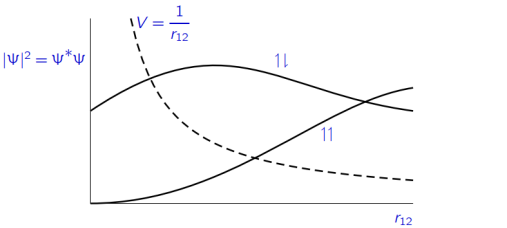
\includegraphics[scale=0.7]{fig/lzhx/微信图片_20211030111438.png}
\end{center}

三重态电子在$r_{12}=0$时分布概率为0,且从图像上来看,自旋平行的电子在空间上倾向于相互远离。而单重态电子在$r_{12}=0$时仍有分布,最大分布概率对应的$r_{12}$存在,也即我们一般认识的轨道半径。三重态在$r_{12}=0$的情况被称作Fermi hole。

\section{原子光谱}
由于轨道角动量和自旋都具有角动量的量纲,所以没什么理由这两个量不会耦合在一起,尤其是小到原子尺度下,考虑到电子的德布罗意波长比原子尺寸还大,因此考虑引入旋轨耦合哈密顿量$\hat{H}_{\rm{SO}}$:
\[\hat{H}=\hat{H_0}+\hat{H}_{\rm{SO}}=-\frac{\hbar^2}{2m_e}\sum_i\nabla^2_i+\sum_{i,j}\frac{1}{r_{ij}}+\sum_{i}\xi(r_i)\hat{L}_i\cdot\hat{S}_i\]
如果引入总角动量算符的话$\hat{L}_i \cdot \hat{S}_i$可以被表示为:
\[\hat{\bm{J}}=\hat{\bm{L}}+\hat{\bm{S}} \quad \Rightarrow \quad \hat{\bm{L}}\cdot\hat{\bm{S}}=\sum_i\hat{L}_i\cdot\hat{S}_i=\frac{1}{2}(\hat{\bm{J}}^2-\hat{\bm{L}}^2-\hat{\bm{S}}^2)\]
看似简单了一点,但实际上更麻烦,需要考虑角动量之间的耦合,这又是一个麻烦的话题,以后可能填坑。

这里简单点一下原子光谱项的表示方法(光谱项$^{2s+1}L$,光谱支项$^{2s+1}L_J$)。这里涉及的量子数有轨道的角量子数$l$和电子的自旋量子数$s$,以及两者耦合后的总量子数$J=l+s,l+s-1,\cdots,|l-s|$。其中符号上$L$的部分并不简单为角量子数$l$,而是对应角动量的原子轨道符号的大写,比如$L=S \ (l=1), \ P \ (l=2), \ D \ (l=3)\cdots$。定义一些名词:光谱项的电子多重度$2s+1$,光谱项的总多重度显然是$(2s+1)(2l+1)$,因为是原子体系所有对应于$s$和$l$的$m_s$和$m_l$态简并。每个光谱支项的简并度$m_j=2J+1$。

\subsection{Hund规则}
1、同电子组态,S越大越稳定;

2、S相同,L越大越稳定;

3、L、S相同,若电子数小于半满,J越小越稳定;若电子数大于半满,J越大越稳定。

既然叫了规则,那这玩意儿估计就有不少反例了(笑

\section{多核粒子体系——线性变分法}
对一些复杂的多核粒子体系,我们没有办法通过精确求解薛定谔方程得到其能量与波函数,但是我们可以通过利用现有的精确求解波函数猜测其实际波函数的办法来近似实际体系。一般而言自然体系都会倾向于使得某态的能量尽可能低,我们会假设存在一个最低的基态能量$E_0$,任意的波函数$\ket{\Phi}$作用到哈密顿量上求得的猜测能量$\tilde{E}$都不会比基态能量$E_0$低,可以通过$\tilde{E}$与$E_0$的差距来衡量猜测函数$\ket{\Phi}$的质量好坏。

\[\langle\tilde{E}\rangle=\frac{\bra{\Phi}\hat{H}\ket{\Phi}}{\bra{\Phi}\ket{\Phi}} \geq E_0\]

假设我们知道一组基$\{\ket{\phi_i}\}$,在该基底上可以任意表示一个猜测函数$\ket{\psi}$并带入能量表达式:
\[\ket{\psi}=\sum_ic_i\ket{\phi_i} \ (c_i\in\mathbf{R}) \quad \Rightarrow \quad \langle\tilde{E}\rangle=\frac{\bra{\psi}\hat{H}\ket{\psi}}{\bra{\psi}\ket{\psi}}=\left(\sum_{ij}c_ic_j\bra{\phi_i}\hat{H}\ket{\phi_j}\right)\cdot\left(\sum_{ij}c_ic_j\bra{\phi_i}\ket{\phi_j}\right)^{-1}\]
定义$H_{ij}=\bra{\phi_i}\hat{H}\ket{\phi_j}, \ S_{ij}=\bra{\phi_i}\ket{\phi_j}$,并且对上式做变形:
\[\langle\tilde{E}\rangle\sum_{ij}c_ic_jS_{ij}=\sum_{ij}c_ic_jH_{ij}\]
为了找到使得$\langle\tilde{E}\rangle$最小的系数组$c_i$,我们需要$\langle\tilde{E}\rangle$对系数组$c_i$的偏导值等于0,二阶偏导矩阵正定:
\[\pdv{\langle\tilde{E}\rangle}{c_i}\sum_{ij}c_ic_jS_{ij}+2\langle\tilde{E}\rangle\sum_{j}c_jS_{ij}2=\sum_{j}c_jH_{ij} \quad \Rightarrow \quad \pdv{\langle\tilde{E}\rangle}{c_i}\sum_{ij}c_ic_j\bra{\phi_i}\ket{\phi_j}=2\sum_{j}c_j\left(H_{ij}-\langle\tilde{E}\rangle S_{ij}\right)\]
\[\pdv{\langle\tilde{E}\rangle}{c_i}=0 \quad \Leftrightarrow \quad \sum_{j}\left(H_{ij}-\langle\tilde{E}\rangle S_{ij}\right)c_j=0, \quad (i=1,2,3 \cdots)\]
写成矩阵形式:
\[\begin{pmatrix}
H_{11}-\langle\tilde{E}\rangle S_{11} & H_{12}-\langle\tilde{E}\rangle S_{12} & \ldots & H_{1n}-\langle\tilde{E}\rangle S_{1n}\\
H_{21}-\langle\tilde{E}\rangle S_{21} & H_{22}-\langle\tilde{E}\rangle S_{22} & \ldots & H_{2n}-\langle\tilde{E}\rangle S_{2n}\\
\vdots & \vdots & \ddots & \vdots\\
H_{n1}-\langle\tilde{E}\rangle S_{n1} & H_{n2}-\langle\tilde{E}\rangle S_{n2} & \ldots & H_{nn}-\langle\tilde{E}\rangle S_{nn}\\
\end{pmatrix}
\begin{pmatrix}
c_1\\c_2\\\vdots\\c_n\\
\end{pmatrix}
=0\]
要使得上述齐次方程有解,需要其系数矩阵行列式为0:
\[\begin{vmatrix}
H_{11}-\langle\tilde{E}\rangle S_{11} & H_{12}-\langle\tilde{E}\rangle S_{12} & \ldots & H_{1n}-\langle\tilde{E}\rangle S_{1n}\\
H_{21}-\langle\tilde{E}\rangle S_{21} & H_{22}-\langle\tilde{E}\rangle S_{22} & \ldots & H_{2n}-\langle\tilde{E}\rangle S_{2n}\\
\vdots & \vdots & \ddots & \vdots\\
H_{n1}-\langle\tilde{E}\rangle S_{n1} & H_{n2}-\langle\tilde{E}\rangle S_{n2} & \ldots & H_{nn}-\langle\tilde{E}\rangle S_{nn}\\
\end{vmatrix}=0\]
求解上述行列式我们能得到能量的估计最小值$\langle\tilde{E}\rangle$。

以$H_2^+$为例子,定义符号$\alpha=H_{11}=H_{22}, \ \beta=H_{12}=H_{21}, \ S=S_{12}=S_{21}, \ S_{11}=S_{22}=1$:
\[\begin{vmatrix}
H_{11}-\langle\tilde{E}\rangle S_{11} & H_{12}-\langle\tilde{E}\rangle S_{12} \\
H_{21}-\langle\tilde{E}\rangle S_{21} & H_{22}-\langle\tilde{E}\rangle S_{22} \\
\end{vmatrix}=
\begin{vmatrix}
\alpha-\langle\tilde{E}\rangle & \beta-\langle\tilde{E}\rangle S \\
\beta-\langle\tilde{E}\rangle S & \alpha-\langle\tilde{E}\rangle \\
\end{vmatrix}=0 \quad \Rightarrow \quad \langle\tilde{E}\rangle=\frac{\alpha-\beta}{1-S} \quad \text{or} \quad \frac{\alpha+\beta}{1+S}\]

两个能量分别反带回去得到轨道:
\[\Phi_+=\frac{1}{\sqrt{2+2S}}(\phi_1+\phi_2) \quad \text{when} \quad \langle\tilde{E}\rangle=\frac{\alpha-\beta}{1-S}, \quad \Phi_-=\frac{1}{\sqrt{2-2S}}(\phi_1-\phi_2) \quad \text{when} \quad \langle\tilde{E}\rangle=\frac{\alpha+\beta}{1+S}\]

值得注意的是$\alpha,\beta<0,S>0$。前两个是描述单个轨道的具有的能量和两轨道之间的相互作用,单体能量$\alpha$是负的,由位力定理$2\langle T \rangle=-\langle V \rangle$说明单体能量是负的,相互作用$\beta$也是负数的是因为相对单个氢原子,$H_2^+$能让电子感受到更负的势能,由位力定理可以知道电子的能量会更低,说明相互作用也是负的。

如果考虑了重叠积分,组成的分子轨道上升的能量比下降的多(重叠积分$S$一般都挺小):
\[\Delta E=\left(\frac{\alpha-\beta}{1-S}-\alpha\right)-\left(\alpha-\frac{\alpha+\beta}{1+S}\right)=\frac{\beta-S\alpha}{1-S}-\frac{\beta-S\alpha}{1+S}=2S \cdot \frac{\alpha S-\beta}{1-S^2}\sim 2S \cdot (-\beta)>0 \quad (S \to 0)\]

\begin{center}
    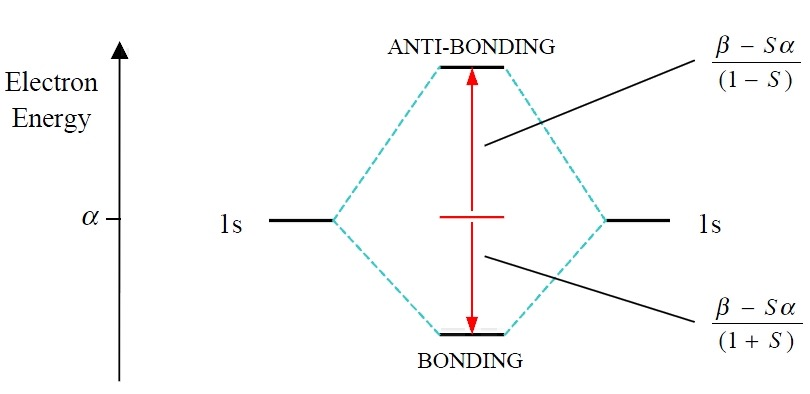
\includegraphics[scale=0.3]{fig/lzhx/Picture1.jpg}
\end{center}

如果我们调整两个氢原子核的间距,可以绘制两个态的势能面:
\begin{center}
    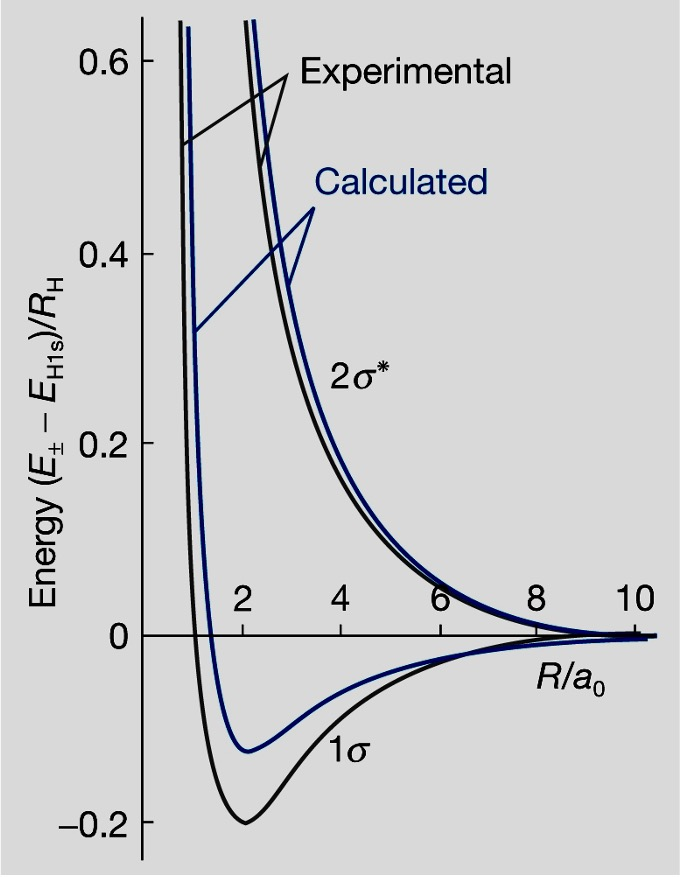
\includegraphics[scale=0.21]{fig/lzhx/Picture2.jpg}
\end{center}

虽然我们没有带入具体的数值计算,但是忽略掉这个小细节,可以看到即使只有两个轨道我们也能绘制出相对接近真实的势能面。现在我们回到两个态的名字,成键和反键,成键的势能面随着原子间距从无穷远渐小逐渐降低,在差不多2倍氢原子半径处达到能量的最低值,然后随着原子核再接近由于核之间的斥力成键能量上升。而反键轨道的势能面则是随着原子间距减小而疯狂上涨。因此我们也把成键轨道的势能面称为束缚态,反键轨道的势能面为解离态。

现在我们关注一下这两个轨道在空间中的分布情况(两套原子坐标得积分掉一套):
\[\rho=\int_{\mathbb{R}^3}|\Phi|^2\dd{^3\bm{r}} \quad \Rightarrow \quad \rho_+=\frac{1}{2+2S}\int_{\mathbb{R}^3}\left(\phi_1^2+\phi_2^2+2\phi_1\phi_2\right)\dd{^3\bm{r}}, \quad \rho_-=\frac{1}{2-2S}\int_{\mathbb{R}^3}\left(\phi_1^2+\phi_2^2-2\phi_1\phi_2\right)\dd{^3\bm{r}}\]

\begin{figure}[htbp]
    \centering
    \begin{minipage}[t]{0.48\textwidth}
    \centering
    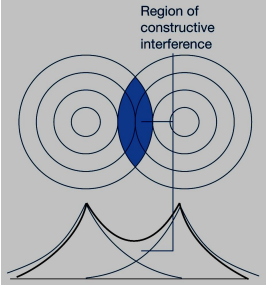
\includegraphics[width=5cm]{fig/lzhx/微信图片_20211102112346.png}
    \caption{$\rho_+$的分布图像}
    \end{minipage}
    \begin{minipage}[t]{0.48\textwidth}
    \centering
    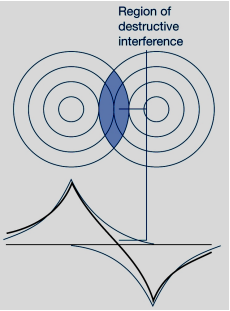
\includegraphics[width=5cm]{fig/lzhx/微信图片_202111021123461.png}
    \caption{$\rho_-$的分布图像}
    \end{minipage}
\end{figure}

\section{计算化学入门前的垫脚石上的艹}
\subsection{Hartree-Fock方法}\label{sec:hf}
我们都知道一个孤立微观系统的哈密顿如下:
\[\hat{H}=\hat{T}_N+\hat{T}_e+\hat{V}_{Ne}+\hat{V}_{ee}+\hat{V}_{NN}\]
在BO近似后,$\hat{T}_N$从电子哈密顿中被移除,$\hat{V}_{NN}$给定核位置后是个常数,可以不包含在电子哈密顿中,但一般来说都还是算的。
\[\hat{H}_{el}=\hat{T}_e+\hat{V}_{Ne}+\hat{V}_{ee}+\hat{V}_{NN}=\sum_i\left(-\frac{1}{2}\nabla^2_i+\sum_N\frac{Z}{r_{Ni}}\right)+\sum_{i<j}\frac{1}{r_{ij}}+V_{NN}\]

虽然我们已经把核项给舍去了,但电子部分的哈密顿依然是一个多体哈密顿,还是一个难以求解的问题。
我们一般能处理的都是单体问题,比如氢原子的电子薛定谔、谐振子等等,所以我们希望能将多体问题尽可能精确地转换为单体问题来处理,如我们考虑平均场近似,即将其他电子对该电子的两体作用考虑为一个等效场:
\[\hat{H}_{el} \approx \sum_i\left(-\frac{1}{2}\nabla^2_i+\sum_N\frac{Z}{r_{Ni}}+\hat{v}_i\right)+V_{NN}:=\sum_i\hat{F}_i + V_{NN}\]

如此一来,上述多电子问题就被转换为了单电子问题,多体哈密顿量被转换单体哈密顿量的加和,理所当然,该体系的波函数也变成了几个单体波函数(自旋轨道)的乘积Hartree积:
\[\Psi = \psi_1(1)\psi_2(2)\cdots\psi_n(n)=\prod_i\psi_i(i)\]

由于电子费米子的全同性的要求,上述需要对Hartree基做反对称化得到Slater行列式:
\[\Psi=\frac{1}{\sqrt{n!}}
    \begin{vmatrix}
        u_1(1) & u_2(1) & \ldots & u_n(1)\\
        u_1(2) & u_2(2) & \ldots & u_n(2)\\
        \vdots & \vdots & \ddots & \vdots\\
        u_1(n) & u_2(n) & \ldots & u_n(n)\\
    \end{vmatrix}
\]

可以看到上面我们假定了单体波函数组成的体系波函数是精确的,然后认为哈密顿量是不精确的,由此出发,我们会希望通过不断修正哈密顿量来使得结果更精确,于是就有了MP2、MP4等微扰方法的出现。
另一方面,如果我们认为哈密顿量是精确的,那么就认为波函数是不精确的,从Slater行列式出发我们通过变分方法来求解尽可能精确的波函数,已知能量表达式为:
\[E=\frac{\bra{\Psi}\hat{H}\ket{\Psi}}{\bra{\Psi}\ket{\Psi}}\]

体系波函数满足:
\[\bra{u_i(1)}\ket{u_j(1)}=\delta_{ij}\]

体系哈密顿量为:
\[\hat{H}=\sum_i\left(-\frac{1}{2}\nabla^2_i+\sum_N\frac{Z}{r_{Ni}}\right)+\sum_{i<j}\frac{1}{r_{ij}}+V_{NN}\]

由Condon-Slater规则可知,能量$E$如下所示,其中$\bra{ij}\ket{ij},\bra{ij}\ket{ji}$为库伦积分和交换积分,$\hat{h}_i$包括了动能项和核对电子的势能(单体算符):
\[E=\bra{\varPhi}\hat{H}\ket{\varPhi}=\sum_ih_i+\frac{1}{2}\sum_{i,j}\left(\bra{ij}\ket{ij}-\bra{ij}\ket{ji}\right)\]

得到了能量,我们接下来顺理成章的就该来变分,但这里的变分并不是简单的求极值,而是条件变分,由于波函数的限制我们求变分时需要引入以下条件进行拉格朗日乘数法:
\[\bra{u_i(1)}\ket{u_j(1)}-\delta_{ij}=0\]

定义泛函$\eta(\lambda_{ij})$:
\[\eta(\lambda_{ij})=E+\sum_{i,j}\lambda_{ij}(\bra{u_i(1)}\ket{u_j(1)}-\delta_{ij})\]

由(变分计算量太大而且其他书上有,我就不写了):
\[\frac{\delta\eta(\lambda_{ij})}{\delta u_i}=\frac{\delta}{\delta u_i}\left(E+\sum_{i,j}\lambda_{ij}(\bra{u_i(1)}\ket{u_j(1)}-\delta_{ij})\right)=0\]

得到的变分结果我们记为:
\[\hat{F}\varphi_i=\varepsilon_i\varphi_i \qquad \varepsilon_i=\bra*{u_i}\hat{h}_i+\hat{J}_i-\hat{K}_i\ket*{u_i}\]

其中,$\hat{F}$为Fork算符,$\varepsilon_i$为轨道能量,$\varphi_i$为正则自旋轨道,Fork算符表达式为:
\[\hat{F}_i = \hat{h}_i + \hat{J}_i - \hat{K}_i\]
\[\hat{J}_iu_i(1) = \sum_{j \neq i}\left(\int u_j^*(2)\frac{1}{r_{ij}}u_j(2)\dd{\tau}_2\right)u_i(1) \qquad \hat{K}_iu_i(1) = \sum_{j \neq i}\left(\int u_j^*(2)\frac{1}{r_{ij}}u_i(2)\dd{\tau}_2\right)u_j(1)\]

Fock 算符中电子相互作用项可整体打包成:
\[\sum_i\bra{u_i}(\hat{J}_i-\hat{K}_i)\ket{u_i}=\sum_{ij}(\bra{ij}\ket{ij}-\bra{ij}\ket{ji})\]

当然,单个Slater行列式描述一个多体问题也是有误差的,于是我们希望能进一步地精确波函数,于是就有了CI、CC等方法。

话说回来,由于我们还是给不出每一个自旋轨道的解析式,所以这个方法我们还没办法直接用。

\subsection{Hartree-Fock–Roothaan方法}
如上文所说,我们给不出Hartree-Fock方程所需的体系波函数,所以我们需要用已知的函数去拟合体系波函数,这里给出Roothaan给出的方法,得到的方程称为Hartree-Fock–Roothaan方程:

假定体系波函数可以被已知基组展开,下面的公式中同时会展示矩阵表示,基向量采用行向量表示:
\[\psi_i=\sum_{\nu=1}c_{\nu i}f_{\nu} \qquad (\mathbf{\Psi} = \mathbf{\Phi} \mathbf{C}_{\text{coeff}})\]
将基函数带入Hartree-Fock方程后可以得到如下表达式:
\[\hat{F}\sum_{\nu=1}c_{\nu i}f_{\nu}=\varepsilon_i\sum_{\nu=1}c_{\nu i}f_{\nu}\]
对上述方程等式两边同时左乘一个$f_{\mu}$可以得到
\[\sum_{\nu=1}c_{\nu i}\bra{f_{\mu}}\hat{F}\ket{f_{\nu}}=\varepsilon_i\sum_{\nu=1}c_{\nu i}\bra{f_{\mu}}\ket{f_{\nu}} \quad \text{where} \quad F_{rs}=\bra{f_r}\hat{F}\ket{f_s} \quad \text{and} \quad S_{rs}=\bra{f_r}\ket{f_s}\]

如果把所有波函数都做上述展开,则可写成如下Hartree-Fock–Roothaan方程
\[\mathbf{F}\mathbf{C}=\mathbf{S}\mathbf{C}\varepsilon\]

上述方程组似乎跟我们能解的方程有一点点不一样,我们能处理的是方程组是厄密矩阵(这里是实对称阵)的正交对角化的问题:
\[\mathbf{F}\mathbf{C}'=\mathbf{C}'\varepsilon\]

Fock矩阵也是实对称矩阵,overlap矩阵也是实对称矩阵,我们自然会想到能不能将Hartree-Fock–Roothaan方程转化成上述方程呢?
考虑如下基的酉变换:
\[\phi_i = \sum_{i}U_{ji}f_j \qquad \mathbf{\varPhi}=\mathbf{U}\mathbf{\Psi}\]
其中$\mathbf{U}$为
\[\mathbf{U}=\mathbf{X}\mathbf{s}^{-1/2} \qquad \mathbf{X}^{\dagger}\mathbf{S}\mathbf{X}=\mathbf{s}\]
$\mathbf{X}$,$\mathbf{s}$为$\mathbf{S}$正交对角化的变换矩阵和对角阵,$\mathbf{s}^{-1/2}$为矩阵$\mathbf{s}^{-1}$的开方,其定义为$\mathbf{s}^{-1/2}\mathbf{s}^{-1/2}=\mathbf{s}^{-1}$。

做完如下变换之后,Hartree-Fock–Roothaan方程可以改写成:
\[\mathbf{U}^{\dagger}\mathbf{S}\mathbf{U}\mathbf{C}'=(\mathbf{X}\mathbf{s}^{-1/2})^{\dagger}\mathbf{S}(\mathbf{X}\mathbf{s}^{-1/2})\mathbf{C}'=\mathbf{X}^{\dagger}\mathbf{S}\mathbf{X}\mathbf{s}^{-1}\mathbf{C}'=\mathbf{s}\mathbf{s}^{-1}\mathbf{C}'=\mathbf{C}' \ , \ (\mathbf{C}':=\mathbf{U}^{\dagger}\mathbf{C})\]
\[\mathbf{U}^{\dagger}\mathbf{F}\mathbf{U}\mathbf{C}'=\varepsilon\mathbf{C}' \Rightarrow \mathbf{F}'\mathbf{C}'=\varepsilon\mathbf{C}' \ , \ (\mathbf{F}':=\mathbf{U}^{\dagger}\mathbf{F}\mathbf{U})\]

然后我们就能解这样一个变换后的方程了。
实际上在python中使用scipy.linalg.eigh($\mathbf{F}$,$\mathbf{S}$)就能直接解出$\mathbf{C}$。
但求解Hartree-Fock–Roothaan方程真的只是做一个对角化吗,如果是这样就好了。
我们具体来看每个矩阵的具体形式,系数矩阵和overlap矩阵是简单的,fock矩阵包含了单电子积分和双电子积分:
\[F_{\mu\nu} = \bra*{\phi_{\mu}}\hat{h} + \hat{J} - \hat{K}\ket*{\phi_{\nu}}\]
单电子积分是简单的
\[h_{\mu\nu}=\bra*{\phi_{\mu}}\hat{h}\ket*{\phi_{\nu}}\]
双电子积分我们打包处理
\begin{equation*}
    \begin{aligned}
        \bra*{\phi_{\mu}}\hat{J} - \hat{K}\ket*{\phi_{\nu}} & = \bra*{\phi_{\mu}}\ket{\sum_{j \neq i}\left(\int u_j^*(2)\frac{1}{r_{ij}}u_j(2)\dd{\tau_2}\right)\phi_{\nu}(1)-\sum_{j \neq i}\left(\int u_j^*(2)\frac{1}{r_{ij}}\phi_{\nu}(2)\dd{\tau_2}\right)u_j(1)} \\
         & = \sum_{j}\iint \phi_{\mu}^*(1)u_j^*(2)\left[\frac{1}{r_{ij}}(1-\hat{P}_{12})\right]u_j(2)\phi_{\nu}(1) \dd{\tau_1}\dd{\tau_2} \\
         & = \sum_{\alpha}\sum_{\beta}\sum_{j}c^*_{\alpha j}c_{\beta j}\iint \phi_{\mu}^*(1)\phi_{\alpha}^*(2)\left[\frac{1}{r_{ij}}(1-\hat{P}_{12})\right]\phi_{\beta}(2)\phi_{\nu}(1) \dd{\tau_1}\dd{\tau_2} \\
         & = \sum_{\alpha}\sum_{\beta}P_{\alpha\beta}\iint \phi_{\mu}^*(1)\phi_{\alpha}^*(2)\left[\frac{1}{r_{ij}}(1-\hat{P}_{12})\right]\phi_{\beta}(2)\phi_{\nu}(1) \dd{\tau_1}\dd{\tau_2} \\
         & = \sum_{\alpha}\sum_{\beta}P_{\alpha\beta}\bra{\phi_{\mu}\phi_{\alpha}}\ket{|\phi_{\beta}\phi_{\nu}}
    \end{aligned}
\end{equation*}
这里我们定义了一个新符号:
\[\bra{\phi_{\mu}\phi_{\alpha}}\ket{|\phi_{\nu}\phi_{\beta}}=\bra{\phi_{\mu}\phi_{\alpha}}\ket{\phi_{\beta}\phi_{\nu}}-\bra{\phi_{\mu}\phi_{\alpha}}\ket{\phi_{\nu}\phi_{\beta}}\]
用来表示库伦积分减去交换积分。

$P_{\alpha\beta}$是密度矩阵的矩阵元,显然我们知道密度矩阵可以由系数矩阵得到$\mathbf{P}=\mathbf{C}\mathbf{C}^{\dagger}$,所以事实上,我们得到的类似矩阵对角化的一个方程实际上也不像是看起来的那么简单,对这样的方程我们没办法直接求解,于是我们选择万能的迭代。
迭代需要一个初猜,在这里也就是初始的密度矩阵(给初猜也是技术活),然后通过对角化更新密度矩阵,反复迭代直到密度矩阵不再变化,这也就是SCF过程。
\[\mathbf{F}(\mathbf{C}')\mathbf{C}'=\mathbf{C}'\varepsilon\]

关于Hartree-Fock方法更多的内容推荐大家阅读\textbf{Szabo前三章},也希望各位能够自己写一个程序来实现(doge),这里提供两个实例:
\href{https://github.com/yangdatou/hf-tutorial}{大头版HF (积分算好了) }和
\href{https://github.com/Walter-Feng/Hartree-Fock-in-CPP}{叔叔版HF (从基组开始嗯造)}。

Hartree-Fock–Roothaan方程还有另外一个形式,以密度矩阵形式体现
\[\mathbf{F}\mathbf{P}\mathbf{S}=\mathbf{S}\mathbf{P}\mathbf{F}\]

证明上述方程与Hartree-Fock–Roothaan方程等价之前先介绍密度矩阵的几个性质
\[1. \ \mathbf{P}=\mathbf{P}^{\dagger} \qquad 2. \ \mathbf{P}\mathbf{S}\mathbf{P}=\mathbf{P} \qquad 3.\ \text{Tr}(\mathbf{P}\mathbf{S})=N\]

开始证明
\[\mathbf{F}\mathbf{C}=\varepsilon\mathbf{S}\mathbf{C} \quad \Rightarrow \quad \mathbf{F}\mathbf{C}(\mathbf{S}\mathbf{C})^{\dagger}=\varepsilon\mathbf{S}\mathbf{C}(\mathbf{S}\mathbf{C})^{\dagger} \quad \Rightarrow \quad \mathbf{F}\mathbf{P}\mathbf{S}=\varepsilon\]
\[\mathbf{F}\mathbf{C}=\varepsilon\mathbf{S}\mathbf{C} \quad \Rightarrow \quad \mathbf{F}\mathbf{C}(\mathbf{F}\mathbf{C})^{\dagger}=\varepsilon\mathbf{S}\mathbf{C}(\mathbf{F}\mathbf{C})^{\dagger} \quad \Rightarrow \quad \mathbf{I}=\varepsilon\mathbf{S}\mathbf{P}\mathbf{F} \quad \Rightarrow \quad \mathbf{I}=(\varepsilon\mathbf{S}\mathbf{P}\mathbf{F})^{\dagger} \quad \Rightarrow \quad \mathbf{S}\mathbf{P}\mathbf{F}=\varepsilon^{\dagger}=\varepsilon\]

基于上述形式的自洽场方程可以介绍DIIS辣!


\subsection{部分基组}
\paragraph*{Slater-type orbitals (STO's)}
\[\phi_{abc}^{\rm{STO}}(x,y,z)=Nx^ay^bz^ce^{-\zeta r}\]

其中,$N$为归一化系数,且a,b,c被角动量控制:$a+b+c=L$,在远距离与近距离行为拟合实际波函数较好。长得跟氢原子波函数形式相近但是缺乏节点且不完全球谐,且收敛慢。

\paragraph*{Gaussian-type orbitals (GTO's)}
\[\phi_{abc}^{\rm{GTO}}(x,y,z)=Nx^ay^bz^ce^{-\zeta r^2}\]

其中,$N$为归一化系数,且a,b,c被角动量控制:$a+b+c=L$。收敛快且有多种方法处理,长得跟氢原子波函数完全不一样。单个函数在近距离行为相较于 Slater 函数拟合实际波函数较差,解决办法是用多个函数来逼近 Slater 函数。比如最常见的 STO-3G 是用三个 GTO 来拟合一个 STO。

\begin{center}
    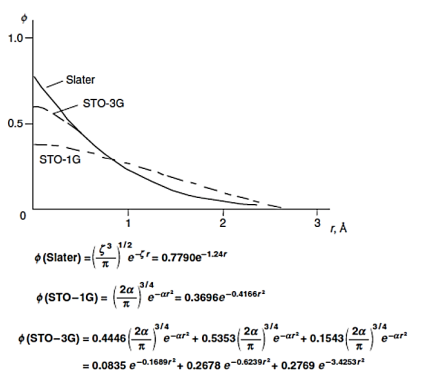
\includegraphics{fig/lzhx/微信图片_20211102165150}
\end{center}

下面给出的是 STO-3G 描述不同原子需要的函数个数,一般而言 STO-3G 都是作为计算体系的极小基:
\begin{center}
    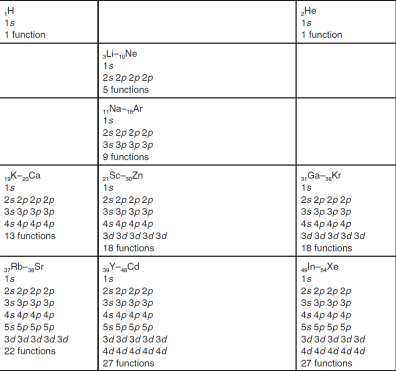
\includegraphics[scale=0.7]{fig/lzhx/微信图片_20211102171332.png}
\end{center}

\paragraph*{Contracted Gaussian type orbitals (CGTO's)}
\[\phi_{abc}^{\rm{CGTO}}(x,y,z)=N\sum_{i=1}^n x^ay^bz^ce^{-\zeta r^2}\]

在现在的基组构建中 CGTO 也可以用来代替单个 GTO,提升优化效率。

\paragraph*{3–21G Split Valence and Double-Zeta Basis Set}
在这种基组下,我们把电子分为两种,核层(core orbitals)与价层(valence orbital),内层的轨道每一个轨道用一个包含三个Gaussian函数的基函数描述,价层每个轨道分为内层与外层,内层(inner shell)用两个Gaussian函数描述,外层(outer shell)用一个Gaussian函数描述:
\begin{center}
    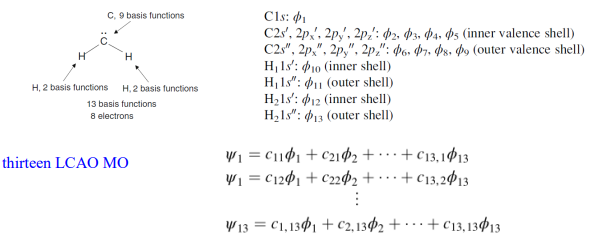
\includegraphics[scale=0.9]{fig/lzhx/微信图片_20211102172815}
\end{center}
\begin{center}
    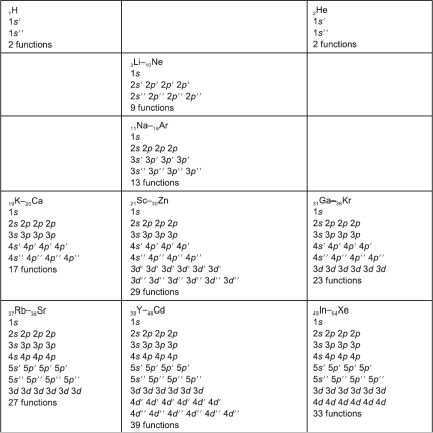
\includegraphics[scale=0.7]{fig/lzhx/微信图片_202111021728151}
\end{center}

\paragraph*{极化函数}
极化函数是角动量相对更大的函数。将它们添加到基组中,可以增加轨道的可极化性,多Zeta基组使轨道在径向上的分布变得灵活,极化函数使轨道在角度上的分布能够具有更大的变形性,更接近真实分子中电子云变形情况,因此计算精度会得到明显提高。
\begin{center}
    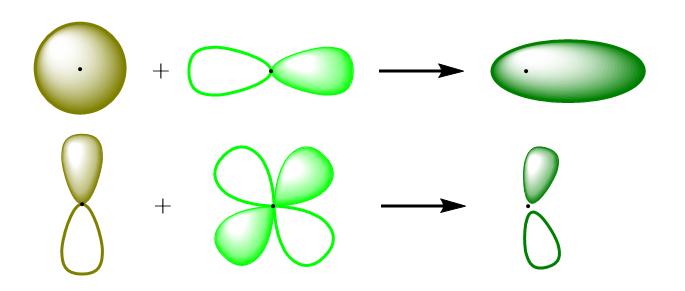
\includegraphics[scale=0.4]{fig/lzhx/polarization.png}
\end{center}
比如6-31g(d)/6-31g(d,p)或者6-31g*/6-31g**,这两套符号表示的是一个意思,分别表示给重原子(5个)加一套d轨道和给重原子加一套d轨道(5个)给氢原子加一套p轨道(3个)。
\paragraph*{弥散函数}
是空间分布更广、更松软的函数(一个指数悉数极小的GTO),一般来说当研究对象为阴离子,或考察体系的弱相互作用、偶极矩、极化率等方面时需要加入此类函数。但这类函数的弥散实在是太广了,以至于物理意义很难评估,并且极大地增加了计算量,所以弥散函数要慎加。

比如6-31+g/6-31++g,分别表示给重原子的每个价层加一个弥散函数和给重原子的每个价层加一个弥散函数给氢原子的每个价层加一个弥散函数。



\section{分子光谱}
在BO近似后,我们考虑一个分子的能量由平动、转动、振动、电子能量组成:
\[E=E_{\rm{trans}}+E_{\rm{rot}}+E_{\rm{vib}}+E_{\rm{el}}\]
\begin{center}
    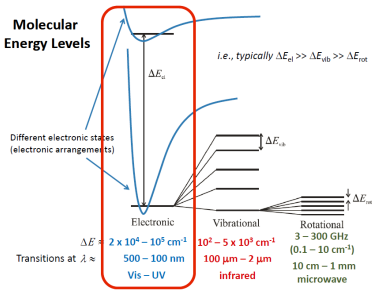
\includegraphics{fig/lzhx/微信图片_20211102175446.png}
\end{center}

与原子光谱类似,分子光谱也有类似的表达方式:
\[M^S\Lambda^{(+/-)}_\Omega\]

其中,$s$、$\Lambda$、$\Omega$由下式给出:
\[S=2s+1 \qquad \hat{J}_z\varPsi=\Lambda\varPsi \qquad \Omega=|\Lambda+S| \qquad \Lambda=\sum_ij_i \qquad S=\sum_iS_i\]

$\Lambda$的取值如下,判断的方法是看开壳层电子所在轨道的$j$值的矢量叠加:
\[\Lambda=0 \ \rightarrow \ \Sigma, \quad \Lambda=\pm 1 \ \rightarrow \ \Pi, \quad \Lambda=\pm 2 \ \rightarrow \ \Delta, \quad \cdots\]

$\Omega$的结果通常用$g$或者$u$来表示,其取值可以通过判断$u$轨道上的单电子个数来判断——每一个在$u$上的电子其对称性都记为$u$,总的$\Omega$取值通过以下方式将各个$u$通过结合运算合成:
\begin{center}
    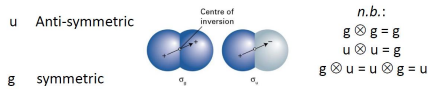
\includegraphics{fig/lzhx/微信图片_20211106011930.png}
\end{center}

分子谱相中右上角的角标$+/-$仅在$\Lambda$取值为$\Sigma$时显现,其取值由波函数轨道部分对称或反对称决定:对称时为+,反之为-。

$M$为按能量从低到高用符号$X$、$A$、$B$$\cdots$来表示,如:$X^3\Sigma^-_g$、$A^1\nabla^2_g$、$B^1\Sigma^+_g$。

谱相的多重度为:
\[2(2s+1) \ (\Lambda \neq 0), \quad 2s+1 \ (\Lambda = 0)\]

\subsection{双原子分子光谱实例}
如果不考虑将电子激发到其他能级上,$O_2$分子可能的开壳层排布为:
\[
    \begin{array}{lcccccc}
        state & \pi_+(\alpha\beta)\pi_- & \pi_+(\alpha)\pi_-(\alpha) & \pi_+(\alpha)\pi_-(\beta) & \pi_+(\beta)\pi_-(\alpha) & \pi_+(\beta)\pi_-(\beta) & \pi_+\pi_-(\alpha\beta) \\
        M_L=  & 2 & 0 & 0 & 0 & 0 & -2 \\
        M_S=  & 0 & 1 & 0 & 0 & -1 & 0
    \end{array}
\]

当然,这么写是并不完全合理,由于全同性,对于对应相同谱相的电子组态我们无法区分,如1、6,3、4三对电子组态,因此,在正式确定对应于同一个谱相的电子组态时,我们需要按照波函数反对称化以及粒子全同性的要求将其两两线性组合。

如对1、6这组,首先写出其价层的$Slater$行列式,并定义简写:
\[
\varphi_1=\frac{1}{\sqrt{2}}
\begin{vmatrix}
    \pi_{g+}(1)\alpha(1) & \pi_{g+}(1)\beta(1) \\
    \pi_{g+}(2)\alpha(2) & \pi_{g+}(2)\beta(2)
\end{vmatrix}
:=
\begin{vmatrix}
    \pi_{g+}(1)\alpha(1) & \pi_{g+}(2)\beta(2)
\end{vmatrix}
\]
\[
\varphi_6=\frac{1}{\sqrt{2}}
\begin{vmatrix}
    \pi_{g-}(1)\alpha(1) & \pi_{g-}(1)\beta(1) \\
    \pi_{g-}(2)\alpha(2) & \pi_{g-}(2)\beta(2)
\end{vmatrix}
:=
\begin{vmatrix}
    \pi_{g-}(1)\alpha(1) & \pi_{g-}(2)\beta(2)
\end{vmatrix}
\]

由于我们指定了这两个电子排布在某个确定角动量的轨道上,这不符合粒子全同性的要求,当然更本质的原因是这两个波函数不是$\hat{S}^2$的本征函数,其自旋无意义,这里需要对两个态进行正交线性组合:
\[\Psi=\frac{1}{\sqrt{2}}(\varphi_1+\varphi_6) \qquad \Psi'=\frac{1}{\sqrt{2}}(\varphi_1-\varphi_6)\]

\[|M_L|=2 \qquad |M_S|=0 \qquad g \times g=g\]

故,这两组电子组态对应的分子谱项为:$^1\nabla^2_g$

同理,对2、5组:
\[
\varphi_2=\frac{1}{\sqrt{2}}
\begin{vmatrix}
    \pi_{g+}(1)\alpha(1) & \pi_{g-}(1)\alpha(1) \\
    \pi_{g+}(2)\alpha(2) & \pi_{g-}(2)\alpha(2)
\end{vmatrix}
=\frac{1}{\sqrt{2}}
\begin{vmatrix}
    \pi_{g+}(1) & \pi_{g-}(1) \\
    \pi_{g+}(2) & \pi_{g-}(2)
\end{vmatrix}
\alpha(1)\alpha(2)
\]
\[
\varphi_5=\frac{1}{\sqrt{2}}
\begin{vmatrix}
    \pi_{g+}(1)\beta(1) & \pi_{g-}(1)\beta(1) \\
    \pi_{g+}(2)\beta(2) & \pi_{g-}(2)\beta(2)
\end{vmatrix}
=\frac{1}{\sqrt{2}}
\begin{vmatrix}
    \pi_{g+}(1) & \pi_{g-}(1) \\
    \pi_{g+}(2) & \pi_{g-}(2)
\end{vmatrix}
\beta(1)\beta(2)
\]

这两种状态并不违反粒子全同性,故无需重新线性组合,他们对应相同的光谱项。
\[|M_L|=0 \qquad |M_S|=2 \qquad g \times g=g\]

由于轨道波函数部分反对称,故,这两组电子组态对应的分子谱项为:$^3\Sigma_g^-$

对3、4组:
\[
\varphi_3=\frac{1}{\sqrt{2}}
\begin{vmatrix}
    \pi_{g+}(1)\alpha(1) & \pi_{g-}(1)\alpha(1) \\
    \pi_{g+}(2)\beta(2) & \pi_{g-}(2)\beta(2)
\end{vmatrix}
=\frac{1}{\sqrt{2}}
\begin{vmatrix}
    \pi_{g+}(1) & \pi_{g-}(1) \\
    \pi_{g+}(2) & \pi_{g-}(2)
\end{vmatrix}
\alpha(1)\beta(2)
\]
\[
\varphi_4=\frac{1}{\sqrt{2}}
\begin{vmatrix}
    \pi_{g+}(1)\beta(1) & \pi_{g-}(1)\beta(1) \\
    \pi_{g+}(2)\alpha(2) & \pi_{g-}(2)\alpha(2)
\end{vmatrix}
=\frac{1}{\sqrt{2}}
\begin{vmatrix}
    \pi_{g+}(1) & \pi_{g-}(1) \\
    \pi_{g+}(2) & \pi_{g-}(2)
\end{vmatrix}
\beta(1)\alpha(2)
\]

显然,这样的排布不满足全同性的要求,重新线性组合得到:
\[\Psi=\frac{1}{2}(\pi_{g+}(1)\pi_{g-}(2)-\pi_{g-}(1)\pi_{g+}(2))(\alpha(1)\beta(2)+\beta(1)\alpha(2))\]
\[\Psi'=\frac{1}{2}(\pi_{g+}(1)\pi_{g-}(2)+\pi_{g-}(1)\pi_{g+}(2))(\alpha(1)\beta(2)-\beta(1)\alpha(2))\]
\[|M_L|=0 \qquad |M_S|=2 \qquad g \times g=g\]

考虑轨道部分,对$\Psi$,其最外层轨道部分反对称,故右上角表为-,同理$\Psi$右上角表为+,注意到$\Psi$的自选部分为三重态,故其左上角标为3而非单重态的1:
\[\Psi \ \rightarrow \ ^3\Sigma_g^-, \quad \Psi' \ \rightarrow \ ^1\Sigma_g^+\]

最后,按能量高低给氧分子的三个谱相表上相应符号:
\begin{center}
    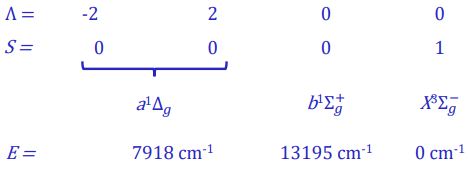
\includegraphics{fig/lzhx/微信图片_20211106140136.png}
\end{center}

\section{微扰理论}
\subsection{非简并定态微扰理论}
对 BO 近似后的定态的电子薛定谔方程,由于双体项的存在我们无法去精确求解该体系的波函数和能量,为此在\ref{sec:hf}小节里我们介绍了 Hartree-Fock 方法,使用近似的哈密顿量$\hat{H}_0$来替代原本精确的哈密顿量$\hat{H}$:
\[\hat{H}=\sum_{i}\hat{h}_i+\sum_{ij}\hat{V}_{ij}=\left(\sum_{i}\hat{F}_i\right)+\left(\sum_{ij}\hat{V}_{ij}-\sum_{i}\hat{F}_i\right)=\hat{H}_0+\hat{H}'\]
如果想在精度上更进一步,我们必须要考虑偏差的哈密顿量$\hat{H}'$,但是由于直接求解过于复杂(本来就是因此舍弃掉这部分)我们可以考虑使用微扰的方法,利用已知的稍微不那么精确的结果去逼近更精确的结果。

微扰能够成立的原理支撑是我们在最开始的一小节\ref{sec:space}提到的\textcolor{blue}{\textbf{算符的本征态张成的空间是完备的}}。我们假设在$\hat{H}_0$的本征态构成的空间是完备的足以用来表达精确的态。理论上只需要一次修正就能拿到完全精确的结果,但由于实操中我们都只能在有限维空间中处理,相对应地修正次数就得达到无穷,即用无穷级数来展开精确态,而且需要偏差哈密顿的影响一般上要比较小的,为此引入微扰参数$\lambda\neq0$把哈密顿量、态和能量改写成:
\[\hat{H}=\hat{H}_0+\lambda\hat{H}‘, \quad \ket{\psi_n}=\sum_{i=0}^{+\infty}\ket{\psi_n^{(i)}}\lambda^i, \quad E_n=\sum_{i=0}^{+\infty}E_n^{(i)}\lambda^i, \quad \hat{H}_0\ket{\psi_n^{(0)}}=E_n^{(0)}\ket{\psi_n^{(0)}}\]

其中$\ket{\psi_n^{(i)}}$、$E_n^{(i)}$为$\ket{\psi_n}$、$E_n$的$i$阶修正,其中对任意的$i,j$满足$i,j$不同时为0:
\[1=\bra{\psi_n}\ket{\psi_n}=\left(\sum_{i=0}^{+\infty}\bra{\psi_n^{(i)}}\lambda^i\right)\left(\sum_{i=0}^{+\infty}\ket{\psi_n^{(i)}}\lambda^i\right)=\bra{\psi_n^{(0)}}\ket{\psi_n^{(0)}}+\cdots=1 +\cdots \quad \Rightarrow \quad \bra{\psi_n^{(i)}}\ket{\psi_n^{(j)}}=0\]
这里利用了实函数内积的非负性,我们称上述结论为微扰态的中间正交性。

将微扰展开的态和能量带入微扰展开的哈密顿方程可得:
\[(\hat{H}_0+\lambda\hat{H}‘)\sum_{i=0}^{+\infty}\ket{\psi_n^{(i)}}\lambda^i=\sum_{i=0}^{+\infty}E_n^{(i)}\lambda^i\sum_{i=0}^{+\infty}\ket{\psi_n^{(i)}}\lambda^i\]
展开取相同的微扰阶数$k$(等式两边$\lambda$的指数)可得(只研究前两阶微扰就好):
\[\begin{aligned}
k=1: \quad & \hat{H}_0\ket{\psi_n^{(1)}}+\hat{H}'\ket{\psi_n^{(0)}}=E_n^{(0)}\ket{\psi_n^{(1)}}+E_n^{(1)}\ket{\psi_n^{(0)}}\\
k=2: \quad & \hat{H}_0\ket{\psi_n^{(2)}}+\hat{H}'\ket{\psi_n^{(1)}}=E_n^{(0)}\ket{\psi_n^{(2)}}+E_n^{(1)}\ket{\psi_n^{(1)}}+E_n^{(2)}\ket{\psi_n^{(0)}}
\end{aligned}\]

对一阶微扰方程两边都内积上$\bra{\psi_n^{(0)}}$,利用中间正交性化简得到能量的一阶修正:
\[\bra{\psi_n^{(0)}}\hat{H}_0\ket{\psi_n^{(1)}}+\bra{\psi_n^{(0)}}\hat{H}'\ket{\psi_n^{(0)}}=E_n^{(0)}\bra{\psi_n^{(0)}}\ket{\psi_n^{(1)}}+E_n^{(1)}\bra{\psi_n^{(0)}}\ket{\psi_n^{(0)}} \quad \Rightarrow \quad E_n^{(1)}=\bra{\psi_n^{(0)}}\hat{H}'\ket{\psi_n^{(0)}}\]

进一步的,如果想获得一阶修正的波函数,我们可以利用上文提到的完备性假设,用零阶波函数来展开一阶波函数,并带入一阶方程:
\[\ket{\psi_n^{(1)}}=\sum_{k\neq n}c_{nk}^{(1)}\ket{\psi_k^{(0)}}\]
\[\begin{aligned}
\sum_{m\neq k}c_{nk}^{(1)}\hat{H}_0\ket{\psi_k^{(0)}}+\hat{H}'\ket{\psi_n^{(0)}}&=E_n^{(0)}\sum_{k\neq n}c_{nk}^{(1)}\ket{\psi_k^{(0)}}+E_n^{(1)}\ket{\psi_n^{(0)}} \\ 
\sum_{k\neq k}c_{nk}^{(1)}\left(\hat{H}_0-E_n^{(0)}\right)\ket{\psi_k^{(0)}}&=-(\hat{H}'-E_n^{(1)})\ket{\psi_n^{(0)}}
\end{aligned}\]
假设零阶微扰态正交归一$\bra{\psi_m^{(0)}}\ket{\psi_k^{(0)}}=\delta_{mk}$,在方程两边同时内积上$\bra{\psi_m^{(0)}}$得到:
\[\begin{aligned}
\sum_{k\neq n}c_{nm}^{(1)}\bra{\psi_m^{(0)}}\left(\hat{H}_0-E_n^{(0)}\right)\ket{\psi_k^{(0)}}&=-\bra{\psi_m^{(0)}}(\hat{H}'-E_n^{(1)})\ket{\psi_n^{(0)}}\\
\sum_{k\neq n}c_{nm}^{(1)}\bra{\psi_m^{(0)}}\left(E_m^{(0)}-E_n^{(0)}\right)\ket{\psi_k^{(0)}}&=-\bra{\psi_m^{(0)}}(\hat{H}'-E_n^{(1)})\ket{\psi_n^{(0)}}
\end{aligned} \quad \Rightarrow \quad c_{nm}^{(1)}=-\frac{\bra{\psi_m^{(0)}}\hat{H}'\ket{\psi_n^{(0)}}}{E_k^{(0)}-E_n^{(0)}}\]
最终可以得到一阶修正的波函数:
\[\ket{\psi_n^{(1)}}=-\sum_{m\neq n}\frac{\bra{\psi_m^{(0)}}\hat{H}'\ket{\psi_n^{(0)}}}{E_m^{(0)}-E_n^{(0)}}\ket{\psi_m^{(0)}}\]

进一步对二阶微扰方程两边都内积上$\bra{\psi_n^{(0)}}$,利用中间正交性化简得到能量的二阶修正:
\[E_n^{(2)}=\bra{\psi_n^{(0)}}\hat{H}'\ket{\psi_n^{(1)}}=-\sum_{m\neq n}\frac{\bra{\psi_m^{(0)}}\hat{H}'\ket{\psi_n^{(0)}}}{E_m^{(0)}-E_n^{(0)}}\bra{\psi_n^{(0)}}\hat{H}'\ket{\psi_m^{(0)}}=-\sum_{m\neq n}\frac{\left|\bra{\psi_m^{(0)}}\hat{H}'\ket{\psi_n^{(0)}}\right|^2}{E_m^{(0)}-E_n^{(0)}}\]
二阶波函数就不求了(会累死人的,而且后面我就只打算讲讲 MP2 作为例子)。

实际使用来看微扰理论在给出能量的近似时是非常精确的,但对波函数的计算却不是太理想。

\subsection{一阶k重简并定态微扰理论}
当零阶方程出现简并能级时,直接套用非简并的公式会出现除0的无穷大项,因此需要对简并的能级做单独的讨论,这里我们以一阶能量修正为例,假设零阶时能级$E_n^{(0)}$有$k$个经过正交化后的简并态$\ket{\psi_{nj}^{(0)}}$:
\[\ket{\psi_{n}^{(0)}}=\sum_{j=1}^{k}c_j\ket{\psi_{nj}^{(0)}}, \quad (j=1,2,\cdots,k)\]
取其中一个左矢$\bra{\psi_{ni}^{(0)}}$作用到$\ket{\psi_{n}^{(0)}}$对应的一阶方程上并把$\ket{\psi_{n}^{(0)}}$基底$\ket{\psi_{nj}^{(0)}}$上展开:
\[\begin{aligned}
\bra{\psi_{ni}^{(0)}}\hat{H}_0\ket{\psi_{n}^{(1)}}+\bra{\psi_{ni}^{(0)}}\hat{H}'\ket{\psi_{n}^{(0)}}&=E_n^{(0)}\bra{\psi_{ni}^{(0)}}\ket{\psi_{n}^{(1)}}+E_n^{(1)}\bra{\psi_{ni}^{(0)}}\ket{\psi_{n}^{(0)}}\\
\bra{\psi_{ni}^{(0)}}\hat{H}_0\ket{\psi_{n}^{(1)}}+\sum_{j=1}^{k}c_j\bra{\psi_{ni}^{(0)}}\hat{H}'\ket{\psi_{nj}^{(0)}}&=E_n^{(0)}\bra{\psi_{ni}^{(0)}}\ket{\psi_{n}^{(1)}}+E_n^{(1)}\sum_{j=1}^{k}c_j\bra{\psi_{ni}^{(0)}}\ket{\psi_{nj}^{(0)}}\\
\end{aligned}\]
利用中间正交性:
\[\sum_{j=1}^{k}c_j\bra{\psi_{ni}^{(0)}}\hat{H}'\ket{\psi_{nj}^{(0)}}=E_n^{(1)}\sum_{j=1}^{k}c_j\bra{\psi_{ni}^{(0)}}\ket{\psi_{nj}^{(0)}}\]
记$H'_{ij}=\bra{\psi_{ni}^{(0)}}\hat{H}'\ket{\psi_{nj}^{(0)}}, \ (i,j=1,2 \cdot\cdot\cdot k)$,可以将方程组写成矩阵形式:
\[\begin{pmatrix}
H'_{11} & H'_{12} & \ldots & H'_{1n}\\
H'_{21} & H'_{22} & \ldots & H'_{2n}\\
\vdots & \vdots & \ddots & \vdots\\
H'_{n1} & H'_{n2} & \ldots & H'_{nn}\\
\end{pmatrix}
\begin{pmatrix}c_1\\c_2\\\vdots\\c_n\end{pmatrix}
=E_n^{(1)}\begin{pmatrix}c_1\\c_2\\\vdots\\c_n\end{pmatrix}
\ \Leftrightarrow \
\begin{pmatrix}
H'_{11}-E_n^{(1)} & H'_{12} & \ldots & H'_{1n}\\
H'_{21} & H'_{22}-E_n^{(1)} & \ldots & H'_{2n}\\
\vdots & \vdots & \ddots & \vdots\\
H'_{n1} & H'_{n2} & \ldots & H'_{nn}-E_n^{(1)}\\
\end{pmatrix}
\begin{pmatrix}c_1\\c_2\\\vdots\\c_n\end{pmatrix}=0\]
要使得上式子成立只需要系数矩阵的行列式为0:
\[\det(\mathbf{H}'-E_n^{(1)}\mathbf{I})=\begin{vmatrix}
H'_{11}-E_n^{(1)} & H'_{12} & \ldots & H'_{1n}\\
H'_{21} & H'_{22}-E_n^{(1)} & \ldots & H'_{2n}\\
\vdots & \vdots & \ddots & \vdots\\
H'_{n1} & H'_{n2} & \ldots & H'_{nn}-E_n^{(1)}\\
\end{vmatrix}=0\]

上述方法可以解出来一系列不同的一阶能量修正项,如果由于我们一开始说过的,这里只讨论了某个能级$E_n^{(0)}$出现了简并的情况,但实际体系中可能出现多个能级简并的情况,那么之需要重复上述的操作即可计算完全部的$\mathbf{E}^{(1)}$。
\[E_n^{(1)}=\bra{\psi_n^{(0)}}\hat{H}'\ket{\psi_n^{(0)}}\]

回忆一下一阶能量修正的公式,很显然如果把每个能量都放到$\ket{\psi_{n}^{(0)}}$基下表示这会是个(块)对角阵。这整个流程大致实现了以下操作:最开始的$\mathbf{E}^{(1)}$只是一个块对角的矩阵,这些块来自于简并的能级,然后通过简并态正交化以及上述流程,实现了把这些不是对角阵的块再对角化最终拿到一个完全对角化的一阶修正能量$\mathbf{E}^{(1)}$。

\subsection{量子力学的三种等价表述形式}
这里先介绍一下三种量子力学的等价形式:薛定谔绘景,海森堡绘景和相互作用(狄拉克)绘景。分别以下标$S,H,I$表示。从薛定谔绘景开始,我们之前的介绍都是薛定谔绘景下的(不然为什么叫薛定谔方程)。\textcolor{blue}{\textbf{薛定谔绘景认为哈密顿量是不演化(含时)的,而态是演化(含时)的}},考虑时间演化算符$\hat{U}(t)\equiv\hat{U}(t,0)$:
\[i\hbar\pdv{t}\ket{\psi(\bm{r},t)}_S=\hat{H}_S\ket{\psi(\bm{r},t)}_S, \quad \ket{\psi(\bm{r},t)}_S=\hat{U}(t)\ket{\psi(\bm{r},0)}_S \quad \Rightarrow \quad i\hbar\pdv{t}\hat{U}(t)=\hat{H}_S\hat{U}(t)\]
进而可以得出时间演化算符是(哈密顿量是不含时的),其与薛定谔绘景下的哈密顿量$\hat{H}_S$是对易的:
\[\hat{U}(t)=\exp\left(-\frac{i}{\hbar}\int_{0}^{t}\hat{H}_S\dd{t}\right)=\exp\left(-\frac{i\hat{H}_St}{\hbar}\right), \quad [\hat{U}(t),\hat{H}_S]=\exp\left(-\frac{i[\hat{H}_S,\hat{H}_S]t}{\hbar}\right)=0\]
考虑在$t$时刻的算符$\hat{O}$的期望值:
\[\bra{\psi(\bm{r},t)}_S\hat{O}\ket{\psi(\bm{r},t)}_S=\bra{\psi(\bm{r},0)}_S\hat{U}^{\dagger}(t)\hat{O}(0)\hat{U}(t)\ket{\psi(\bm{r},0)}_S=\bra{\psi(\bm{r},0)}_H\hat{O}_H(t)\ket{\psi(\bm{r},0)}_H\]
这里用到了$\ket{\psi(\bm{r},t)}_S=\ket{\psi(\bm{r},0)}_H$初态在哪个表象下都是一样的,之后在相互作用绘景也会用到。同时由于薛定谔绘景的算符$\hat{O}$不包含时间,可以直接认为是海森堡绘景下的初始算符$\hat{O}(0)$。于是我们得到了\textcolor{blue}{\textbf{海森堡绘景,即认为算符是随时间演化的而态不随时间演化}}。算符的演化服从海森堡运动方程:
\[\dv{\hat{O}_H}{t}=-\frac{i}{\hbar}[\hat{O}_H,\hat{H}_S]\]
海森堡运动方程可以从薛定谔绘景的时间演化算符出发推导得到:
\[\dv{\hat{O}_H}{t}=\frac{\partial\hat{U}^{\dagger}(t)}{\partial t}\hat{O}_S\hat{U}(t)+\hat{U}^{\dagger}(t)\hat{O}_S\frac{\partial\hat{U}(t)}{\partial t}=-\frac{i}{\hbar}[\hat{O}_H,\hat{H}_H]=-\frac{i}{\hbar}[\hat{A}_H,\hat{U}^\dagger(t)\hat{U}(t)\hat{H}_S]=-\frac{i}{\hbar}[\hat{O}_H,\hat{H}_S]\]

相互作用绘景可以说介于薛定谔绘景和海森堡绘景之间的,因为在\textcolor{blue}{\textbf{相互作用绘景下哈密顿量$\hat{H}(t)$被分为了可以精确求解(不含时)的部分$\hat{H}_0$和复杂的相互作用(含时)的部分$\hat{H}'(t)$,$\hat{H}_0$通过相互作用绘景下的定态演化算符$\hat{U}_0(t)$被吸收到了态里,而$\hat{H}'(t)$通过类似海森堡绘景中的处理变成了相互作用绘景下的哈密顿量$\hat{H}_I(t)$}}:
\[\ket{\psi(\bm{r},t)}_S=\hat{U}_0(t)\ket{\psi(\bm{r},t)}_I=\exp\left(-\frac{i\hat{H}_0t}{\hbar}\right)\ket{\psi(\bm{r},t)}_I\]
将上述态的转换带入薛定谔绘景下的薛定谔方程可以得到相互作用绘景下的薛定谔方程以及运动方程:
\[i\hbar\pdv{t}\ket{\psi(\bm{r},t)}_I=\hat{U}^{\dagger}_0(t)\hat{H}'(t)\hat{U}_0(t)\ket{\psi(\bm{r},t)}_I=\hat{H}_I(t)\ket{\psi(\bm{r},t)}_I, \quad \dv{\hat{O}_I}{t}=-\frac{i}{\hbar}[\hat{O}_I,\hat{H}_0]\]
由上述薛定谔方程,我们可以类似推导出相互作用绘景下的相互作用时间演化算符,而且其显然满足:
\[\hat{U}_I(t)=\exp\left(-\frac{i}{\hbar}\int_{0}^{t}\hat{H}_I\dd{t}\right), \quad \hat{U}(t)=\hat{U}_0(t)\hat{U}_I(t)\]
回到在$t$时刻的算符$\hat{O}$的期望值:
\[\bra{\psi(\bm{r},t)}_S\hat{O}\ket{\psi(\bm{r},t)}_S=\bra{\psi(\bm{r},0)}_S\hat{U}_I^{\dagger}(t)\hat{U}_0^{\dagger}(t)\hat{O}(0)\hat{U}_0(t)\hat{U}_I(t)\ket{\psi(\bm{r},0)}_S=\bra{\psi(\bm{r},0)}_I\hat{O}_I(t)\ket{\psi(\bm{r},0)}_I\]
可以看出三种绘景都是形式一致的,只是量子力学的不同表象罢了(笑

最后遗留一个小问题,由于$\hat{H}_I$含时,我们没法直接写出该时间演化算符的结果,但是可以通过迭代时间演化算符来近似求解,直接对薛定谔方程积分可以得到如下的形式:
\[i\hbar\pdv{t}\ket{\psi(\bm{r},t)}_I=\hat{H}_I(t)\ket{\psi(\bm{r},t)}_I \quad \Rightarrow \quad \ket{\psi(\bm{r},t)}_I=\ket{\psi(\bm{r},0)}_I-\frac{i}{\hbar}\int_{0}^{t}\hat{H}_I\dd{\tau}\ket{\psi(\bm{r},\tau)}_I\]
不断对积分中的态$\ket{\psi_I(\bm{r},\tau)}$进行迭代可以得到如下递推公式:
\[\ket{\psi(\bm{r},t)}_I=\ket{\psi(\bm{r},0)}_I+\sum_{n=1}^{\infty}\left(-\frac{i}{\hbar}\right)^n\int_{0}^t\dd{\tau_n}\int_{0}^{\tau_n}\dd{\tau_{n-1}}\cdots\int_{0}^{\tau_2}\dd{\tau_1}\hat{H}_I(\tau_n)\hat{H}_I(\tau_{n-1})\cdots\hat{H}_I(\tau_1)\ket{\psi(\bm{r},0)}_I\]
此时我们按照相互作用绘景的相互作用时间演化算符的定义把它从上式中扣出来:
\[\hat{U}_I(t)=1+\sum_{n=1}^{\infty}\left(-\frac{i}{\hbar}\right)^n\int_{0}^t\dd{\tau_n}\int_{0}^{\tau_n}\dd{\tau_{n-1}}\cdots\int_{0}^{\tau_2}\dd{\tau_1}\hat{H}_I(\tau_n)\hat{H}_I(\tau_{n-1})\cdots\hat{H}_I(\tau_1)\]
此级数被称为 Dyson 级数,在推各种谱的吸收表达式的时候会用到(哈哈,我反正是看到头秃

\subsection{含时微扰理论}
当考虑一些更实际的体系如原子分子吸收发射时,会遇到哈密顿量中的含时项不可忽略的情况,这时求解该体系就需要考虑含时的薛定谔方程。由于时间项的引入,简并态出现的可能性将大大下降,因此这里我们仅讨论无简并的含时微扰,假设哈密顿为$\hat{H}=\hat{H}_0+\lambda\hat{H}'(t)$。在相互作用绘景下,给定初态(其实就是定态解):
\[i\hbar\pdv{t}\ket{\psi_n(t)}_I=\hat{H}_I\ket{\psi_n(t)}_I, \quad i\hbar\pdv{t}\ket{\psi_n(0)}_I=\hat{H}_I\ket{\psi_n(0)}_I \quad \Leftrightarrow \quad i\hbar\pdv{t}\ket{m}=\hat{H}_I\ket{m}\]

将$\ket{\psi_n(t)}_I$在定态解$\{\ket{m}\}$的基底下展开:
\[\ket{\psi_n(t)}_I=\sum_m\ket{m}\bra{m}\ket{\psi_n(t)}_I=\sum_mc_{nm}(t)\ket{m} \quad \Rightarrow \quad i\hbar\sum_m\pdv{c_{nm}(t)}{t}\ket{n}=\sum_mc_{nm}(t)\hat{H}_I\ket{n}\]
对上式两侧同时内积上$\bra{k}$得到,定义个缩写符号$\omega_{km}=(E_k-E_m)/\hbar$(到达态能量减去出发态能量):
\[\begin{aligned}
i\hbar\pdv{c_{nk}(t)}{t}&=\sum_mc_{nm}(t)\bra{k}\hat{H}_I\ket{m}=\sum_m\lambda c_{nm}(t)\bra{k}\exp\left(\frac{i\hat{H}_0t}{\hbar}\right)\hat{H}'(t)\exp\left(-\frac{i\hat{H}_0t}{\hbar}\right)\ket{m}\\
&=\sum_m\lambda c_{nm}(t)\bra{k}\hat{H}'(t)\ket{m}\exp\left(-\frac{i(E_m-E_k)t}{\hbar}\right)\equiv\sum_m\lambda c_{nm}(t)\bra{k}\hat{H}'(t)\ket{m}e^{i\omega_{km}t}
\end{aligned}\]
将展开系数做微扰展开,并带入上式,这里再提一下:
\[c_{nm}(t)=c_{nm}^{(0)}+\sum_{j=1}^{+\infty}c_{nm}^{(j)}(t)\lambda^i \quad \Rightarrow \quad i\hbar\sum_{j=1}^{+\infty}\pdv{c_{nk}^{(j)}(t)}{t}\lambda^j=\sum_{j=1}^{+\infty}\lambda^j\sum_mc^{(j-1)}_{nm}(t)\bra{k}\hat{H}'(t)\ket{m}e^{i\omega_{km}t}\]

取出一阶修正项,同时假设定态时系统处于态$\ket{n}$,则系数$c^{(0)}_{nm}=\delta_{mn}$:
\[i\hbar\pdv{c_{nk}^{(1)}(t)}{t}=\bra{k}\hat{H}'(t)\ket{n}e^{i\omega_{kn}t} \quad \Rightarrow \quad c_{nk}^{(1)}(t)=\frac{1}{i\hbar}\int_{0}^{t}\bra{k}\hat{H}'(\tau)\ket{n}e^{i\omega_{kn}\tau}\dd{\tau}\]

回看系数$c_{nk}^{(1)}(t)=\bra{k}\ket{\psi_n(t)}_I$的定义我们知道,其平方$P_{n \to k}(t)=|c_{nk}^{(1)}(t)|^2$表示系统在$t$时刻从初态$\ket{n}$跃迁到$\ket{k}$的跃迁概率,通过对跃迁概率求导,我们能知道跃迁的速率,于是我们就能研究动力学辣!

下面我们以一个具体的微扰哈密顿作为展示,假设存在一个电磁场$\bm{E}(t)=\bm{E}\cos{\omega t}$,与体系的偶极$\hat{\bm{\mu}}$相互作用,因此微扰哈密顿可以写成$\hat{H}'=-\hat{\bm{\mu}}\cdot\bm{E}\cos{\omega t}$,负号来自于相互作用是降低体系能量的。则跃迁系数为:
\[c_{nk}^{(1)}(t)=\frac{1}{i\hbar}\int_{0}^{t}\bra{k}\hat{H}'(\tau)\ket{n}e^{i\omega_{kn}\tau}\dd{\tau}=\frac{i}{\hbar}\int_{0}^{t}\bra{k}\hat{\bm{\mu}}\ket{n}\cdot \bm{E}\cos{\omega t}e^{i\omega_{kn}\tau}\dd{\tau}\]
其中$\bm{\mu}_{nk}\equiv\hat{\bm{\mu}}\ket{n}$为跃迁偶极矩,其与电场场强$\bm{E}$与时间无关,可以从积分中提出来:
\[c_{nk}^{(1)}(t)=\frac{i\bm{\mu}_{nk}\cdot\bm{E}}{2\hbar}\int_{0}^{t}(e^{i\omega t}+e^{-i\omega t})e^{i\omega_{kn}\tau}\dd{\tau}=\frac{\bm{\mu}_{nk}\cdot\bm{E}}{2\hbar}\left[\frac{e^{i(\omega_{kn}+\omega)t}-1}{\omega_{kn}+\omega}+\frac{e^{i(\omega_{kn}-\omega)t}-1}{\omega_{kn}-\omega} \right]\]

对光吸收过程,$\omega$为正值(光发射过程相反),当$\omega$在合适范围内,满足:
\[\left|\frac{e^{i(\omega_{kn}+\omega)t}-1}{\omega_{kn} + \omega}\right| \ll \left|\frac{e^{i(\omega_{kn}-\omega)t}-1}{\omega_{mkn}-\omega}\right|\]
故对光吸收过程(delta函数这里用到了$\pi\delta(x)/t=\mathrm{sinc}^2(xt)$,有点跳步可以自己推导):
\[P_{n \to k}(t)=|c_{nk}^{(1)}(t)|^2\approx\frac{|\bm{\mu}_{nk}\cdot\bm{E}|^2}{2\hbar^2}\cdot\frac{1-\cos{(\omega_{kn}-\omega)t}}{(\omega_{kn}-\omega)^2}=\frac{\pi t}{2\hbar^2}|\bm{\mu}_{nk}\cdot\bm{E}|^2\delta(\omega_{kn}-\omega)\]
进而可以计算在$t$时刻从初态$\ket{n}$跃迁到$\ket{k}$的跃迁速率$k_{n \to k}$:
\[k_{n \to k}=\dv{P_{n \to k}(t)}{t}=\frac{\pi}{2\hbar^2}|\bm{\mu}_{nk}\cdot\bm{E}|^2\delta(\omega_{kn}-\omega)=\frac{\pi}{2\hbar}|\bm{\mu}_{nk}\cdot\bm{E}|^2\delta(E_k-E_n-\hbar\omega)\]

从上述公式可以知道只有当满足$\omega=\omega_{kn}$时越迁才会发生。\textcolor{blue}{\textbf{由微扰假定,我们认为外场不影响系统态本身的分布,系统处于能量为$E$的态上的概率由平衡态密度$\rho(E)$给出}}。因此如果我们考察在外场频率$\omega=\omega_{kn}$时,即$E_n-\hbar\omega=E_k$,从初态$\ket{n}$发生的越迁速率,也即从初态$\ket{n}$跃迁到$\ket{k}$的跃迁速率$k_{n \to k}$:
\[k_{n \to k}=\int k_{n \to ?}(E)\rho(E)\dd{E}=\int \frac{\pi}{2\hbar}|\bm{\mu}_{nk}\cdot\bm{E}|^2\delta(E-E_n-\hbar\omega)\rho(E)\dd{E}=\frac{\pi}{2\hbar}|\bm{\mu}_{nk}\cdot\bm{E}|^2\rho(E_k)\]

上述公式也称为费米黄金定则(Fermi golden rule),描述了垂直激发(微扰假设,外场不改变势能面,即定态)的越迁速率。不做一些奇奇怪怪的动力学都可以使用上述公式很方便得描述一些光化学物理过程。

\subsection{MP2}
这里我们介绍前面略过的 Condon-Slater 规则,首先考虑以正交归一的一组自旋轨道在反对称化后的 Slater 行列式作为体系波函数$\ket{\Phi}=\hat{A}(\ket{\phi_1}\otimes\ket{\phi_2}\otimes\cdots\otimes\ket{\phi_n}):=\hat{A}\ket{\phi_1\phi_2\cdots\phi_n}$,反对称化算符显然有一下性质$\hat{A}=\hat{A}^{\dagger}, \ \hat{A}^2=\sqrt{n!}\hat{A}$(把任意一个位置调换算符作用到反对称化的波函数上只能获得其自身)。因此对overlap:
\[\bra{\Phi}\ket{\Phi}=\bra{\phi_1\phi_2\cdots\phi_n}\sum_k\epsilon_k\hat{P}_k\ket{\phi_1\phi_2\cdots\phi_n}=\bra{\phi_1\phi_2\cdots\phi_n}\ket{\phi_1\phi_2\cdots\phi_n}=1\]
只有完全没被调换过粒子编号的态不为0的内积,如果不是相同态的内积$\bra{\Phi}\ket{\Psi}$显然为0。类似的对于单体算符$\hat{h}_i$,如果我们求能量,即要求用相同的态做内积,只有没被调换过的态有非0结果(调换一次两个轨道不一样,调换两次则至少三个,这里不包含调换回来的情况);如果是不同的态作用到单体算符上,则至多只能有一个轨道不一样且该不同的轨道必须包含在单体算符的期望值项里(假设$\ket{\phi_1}\to\ket{\psi_1}$):
\[\bra{\Phi}\sum_{i=1}^{n}\hat{h}_i\ket{\Phi}=\sum_{i=1}^{n}\bra{\phi_i}\hat{h}_i\ket{\psi_i}, \quad \bra{\phi_1\phi_2\cdots\phi_n}\sum_{i=1}^{n}\hat{h}_i\ket{\psi_1\phi_2\cdots\phi_n}=\bra{\phi_1}\hat{h}_1\ket{\psi_1}\]

我们可以把一次对掉的组分叫做ST。对于一个态,对掉一次至少两个轨道不一样,对掉两次(注意不包含换回来)则不一样的更多,对单体算符由于只允许一个轨道不一样所以不可能允许存在对掉一次的组分,对双体算符也只允许对掉一次,因此对于双体算符$\hat{g}_{ij}$的期望值可以很轻易得写出:
\[\bra{\Phi}\sum_{i<j}\hat{g}_{ij}\ket{\Phi}=\sum_{i<j}\bra{\phi_i\phi_j}\hat{g}_{ij}(1-\hat{P}_{12})\ket{\phi_i\phi_j}=\frac{1}{2}\sum_{i,j}\bra{\phi_i\phi_j}\hat{g}_{ij}(1-\hat{P}_{12})\ket{\phi_i\phi_j}\]
当行列式中存在一个/或者两个轨道不一样,那么这两个轨道必须包含在双电子项的积分中,假设分别为$\ket{\phi_1}\to\ket{\psi_1}$和$\ket{\phi_1}\to\ket{\psi_1}, \ \ket{\phi_2}\to\ket{\psi_2}$:
\[\bra{\Phi}\sum_{i<j}\hat{g}_{ij}\ket{\Phi_1}=\sum_{j=1}^n\bra{\phi_1\phi_j}\hat{g}_{1j}(1-\hat{P}_{12})\ket{\psi_1\phi_j}, \quad \bra{\Phi}\sum_{i<j}\hat{g}_{ij}\ket{\Phi_{12}}=\bra{\phi_1\phi_2}\hat{g}_{12}(1-\hat{P}_{12})\ket{\psi_1\psi_2}\]

经过上述讨论,现在我们来看 Hartree-Fock,比如能量$E$,是精确哈密顿量在 Slater 行列式上的期望:
\[E=\bra{\Phi}\hat{H}\ket{\Phi}=\sum_ih_i+\frac{1}{2}\sum_{i,j}\left(\bra{ij}\ket{ij}-\bra{ij}\ket{ji}\right)\]
非微扰哈密顿量是 Fock 算符之和,对应的非微扰能量$E_0$:
\[E_0=\bra{\Phi}\sum_i\hat{F}_i\ket{\Phi}=\bra{\Phi}\sum_i(\hat{h}_i+\hat{J}_i-\hat{K}_i)\ket{\Phi}=\sum_ih_i+\sum_{i,j}\left(\bra{ij}\ket{ij}-\bra{ij}\ket{ji}\right)\]
微扰部分哈密顿量是双电子积分算符与库伦积分算符和交换积分算符之间的差,对应微扰能量$E'$:
\[E'=\bra{\Phi}\sum_{ij}g_{ij}-\sum_i(\hat{J}_i-\hat{K}_i)\ket{\Phi}=\frac{1}{2}\sum_{i,j}\left(\bra{ij}\ket{ij}-\bra{ij}\ket{ji}\right)-\sum_{i,j}\left(\bra{ij}\ket{ij}-\bra{ij}\ket{ji}\right)=-\frac{1}{2}\sum_{i,j}\left(\bra{ij}\ket{ij}-\bra{ij}\ket{ji}\right)\]
可以发现在 Hartree-Fock 中我们使用的能量已经包含了微扰部分的能量,因此 Hartree-Fock 可以认为是 MP1。这也是为什么微扰方法是从 MP2 开始的,MP 方法的思想是由于 Hartree-Fock 是利用所有占据轨道变分的最优解,因此优化 Hartree-Fock 需要考虑引入空轨道,这里用$\ket{\Phi^{ab}_{ij}}$表示用两个空轨道$ab$替换了两个占据轨道$ij$。为什么只考虑一次性激发两个轨道呢?我们可以看看只激发一个轨道的情况,假设把占据轨道$i$激发到空轨道$a$,根据规则可以写出一下式子:
\[\bra{\Phi^{\rm{HF}}}\hat{H}\ket{\Phi^a_i}=\bra{\phi_i}\hat{h}\ket{\phi_a}+\sum_j\bra{ij}\ket{|aj}=\bra{\phi_i}\hat{F}\ket{\phi_a}=\bra{\Phi^{\rm{HF}}}\hat{H}_0\ket{\Phi^a_i} \quad \Rightarrow \quad \bra{\Phi^{\rm{HF}}}\hat{H}'\ket{\Phi^a_i}=0\]
这说明单激发对于修正 Hartree-Fock 能量毫无帮助,上述结论也称为 Brillouin 定理。

利用我们前文在定态非简并微扰的公式可以知道 MP2 能量是:
\[E^{\rm{MP2}}=-\sum_{i<j}^{\rm{occ}}\sum_{a<b}^{\rm{vir}}\frac{\left|\bra{\Phi^{\rm{HF}}}\hat{H}'\ket{\Phi^{ab}_{ij}}\right|^2}{E^{ab}_{ij}-E^{\rm{HF}}}=-\sum_{i<j}^{\rm{occ}}\sum_{a<b}^{\rm{vir}}\frac{\bra{ij}\ket{|ab}^2}{\varepsilon_a+\varepsilon_b-\varepsilon_i-\varepsilon_j}\]
这里稍微解释一下分母,非微扰的哈密顿是一堆 Fock 算符的和,因此对应的非微扰能量就是轨道能量和,因此两个不同 Slater 行列式的非微扰能量差只需要去数有多少轨道不一样。MP2 基本能覆盖80$\sim$90\%的相关能。

\section{附录I:一点数学(微积分线代什么的自己去看书)}
\subsection{变量分离}
变量分离是假设偏微分方程的解可以由几个以不同变量(组)为自变量的函数共同表示,即:
\[y(\bm{r}_1,\bm{r}_2,\cdot\cdot\cdot,\bm{r}_n)=y_1(\bm{r}_1)y_2(\bm{r}_2)\cdot\cdot\cdot y_n(\bm{r}_n)\]

这里,我们以含时薛定谔方程为例,假设解出的波函数$\psi(\bm{r},t)=\varPsi(\bm{r})\phi(t)$,除了平凡解$\psi=0$外,我们可以认为解出的波函数仅在有限个点上取值为零,不考虑这些奇异点,我们将方程两边同时除以$\varphi\phi$:
\[i \hbar \frac{\partial \psi}{\partial t}=\left (-\frac{\hbar^2}{2m}\nabla^2+V \right ) \psi \quad \Rightarrow \quad i \hbar \varphi \frac{\partial \phi}{\partial t}= -\frac{\hbar^2}{2m} \phi \nabla^2 \varPsi+V\varPsi\phi \quad \Rightarrow \quad i \hbar \frac{1}{\phi} \frac{\partial \phi}{\partial t}= -\frac{\hbar^2}{2m} \frac{1}{\varPsi} \nabla^2 \varPsi+V\]
显然我们可以给出一个能量单位的参数$E$使得原方程可以写成以下方程组:
\[\left\{
\begin{array}{r}
i\hbar\frac{1}{\phi}\frac{\partial\phi}{\partial t}=E\\
-\frac{\hbar^2}{2m}\frac{1}{\varPsi}\nabla^2\varPsi+V=E
\end{array} \right. \quad \Rightarrow \quad
\left\{
\begin{array}{l}
\phi(t)=\exp(-\frac{iEt}{\hbar})\\
\hat{H}\varPsi=E\varPsi
\end{array} \right.\]

\subsection{球坐标下的拉普拉斯算符展开}
球坐标与直角坐标的转换关系如下:
\[x=r\sin\theta\cos\phi, \quad y=r\sin\theta\cos\phi, \quad z=r\cos\theta\]
计算某个坐标下的梯度算子$\nabla$可以考虑对坐标向量$\bm{r}=(x,y,z)$求导并归一化得到。如球坐标的单位向量在直角坐标的基底下可以被表示为:
\begin{equation*}
\begin{aligned}
\hat{\bm{r}} &=\pdv{\bm{r}}{r}= (\sin\theta \cos\phi, \sin\theta \sin\phi, \cos\theta), \\
\hat{\bm{\theta}} &=\frac{1}{r}\pdv{\bm{r}}{\theta}= (\cos\theta \cos\phi, \cos\theta \sin\phi, -\sin\theta), \\
\hat{\bm{\phi}} &=\frac{1}{r\sin\theta}\pdv{\bm{r}}{\phi}= (-\sin\phi, \cos\phi, 0).
\end{aligned}
\end{equation*}
因此我们可以写出球坐标下的梯度算子$\nabla$:
\[\nabla=\hat{\bm{r}}\pdv{r}+\hat{\bm{\theta}}\frac{1}{r}\pdv{\theta}+\hat{\bm{\phi}}\frac{1}{r\sin\theta}\pdv{\phi}\]
当我们考虑计算球坐标下的拉普拉斯算子$\Delta=\nabla^2=\nabla\cdot\nabla$时,我们注意到球坐标的单位向量对坐标的导数并非简单的0或者1(在直角坐标系下的情况):
\begin{equation*}
\begin{aligned}
\frac{\partial \hat{\bm{r}}}{\partial r} &=\frac{\partial \hat{\bm{\theta}}}{\partial r}=\frac{\partial \hat{\bm{\phi}}}{\partial r}=0\\
\frac{\partial \hat{\bm{r}}}{\partial \theta} &= (\cos\theta \cos\phi, \cos\theta \sin\phi, -\sin\theta) = \hat{\bm{\theta}}, \\
\frac{\partial \hat{\bm{r}}}{\partial \phi} &= (-\sin\theta \sin\phi, \sin\theta \cos\phi, 0) = \sin\theta \, \hat{\bm{\phi}},\\
\frac{\partial \hat{\bm{\theta}}}{\partial \theta} &= (-\sin\theta \cos\phi, -\sin\theta \sin\phi, -\cos\theta) = -\hat{\bm{r}}, \\
\frac{\partial \hat{\bm{\theta}}}{\partial \phi} &= (-\cos\theta \sin\phi, \cos\theta \cos\phi, 0) = \cos\theta \, \hat{\bm{\phi}},\\
\frac{\partial \hat{\bm{\phi}}}{\partial \theta} &= (0, 0, 0) = \bm{0}, \\
\frac{\partial \hat{\bm{\phi}}}{\partial \phi} &= (-\cos\phi, -\sin\phi, 0) = -\sin\theta \, \hat{\bm{r}} - \cos\theta \, \hat{\bm{\theta}}.
\end{aligned}
\end{equation*}

因此在直角坐标系下的拉普拉斯算子$\nabla^2$可以表示成如下形式:
\[\nabla^2=(\bm{i}\frac{\partial}{\partial{x}}+\bm{j}\frac{\partial}{\partial{y}}+\bm{k}\frac{\partial}{\partial{z}}) \cdot (\bm{i}\frac{\partial}{\partial{x}}+\bm{j}\frac{\partial}{\partial{y}}+\bm{k}\frac{\partial}{\partial{z}})=\frac{\partial^2}{\partial{x}^2}+\frac{\partial^2}{\partial{y}^2}+\frac{\partial^2}{\partial{z}^2}\]
但我们并不能直接将球坐标系下的梯度做点乘得到球坐标下的拉普拉斯算子:
\[\nabla^2=(\hat{\bm{r}}\pdv{r}+\hat{\bm{\theta}}\frac{1}{r}\pdv{\theta}+\hat{\bm{\phi}}\frac{1}{r\sin\theta}\pdv{\phi}) \cdot (\hat{\bm{r}}\pdv{r}+\hat{\bm{\theta}}\frac{1}{r}\pdv{\theta}+\hat{\bm{\phi}}\frac{1}{r\sin\theta}\pdv{\phi}) \neq \frac{\partial^2}{\partial{r^2}}+\frac{1}{r^2}\frac{\partial^2}{\partial{\theta^2}}+\frac{1}{r^2sin^2 \theta }\frac{\partial^2}{\partial{\phi^2}}\]
需要对每一项分别计算,第一项:
\[
\hat{\mathbf{r}}\frac{\partial}{\partial r} \cdot \left(\hat{\mathbf{r}}\frac{\partial}{\partial r}\right) = \hat{\mathbf{r}} \cdot \left(\frac{\partial\hat{\mathbf{r}}}{\partial r}\frac{\partial}{\partial r} + \hat{\mathbf{r}}\frac{\partial^2}{\partial r^2}\right) = \hat{\mathbf{r}} \cdot \hat{\mathbf{r}}\frac{\partial^2}{\partial r^2} = \frac{\partial^2}{\partial r^2}
\]
第二项:
\[
\hat{\mathbf{r}}\frac{\partial}{\partial r} \cdot \left(\hat{\boldsymbol{\theta}}\frac{1}{r}\frac{\partial}{\partial \theta}\right) = \hat{\mathbf{r}} \cdot \left(\frac{\partial\hat{\boldsymbol{\theta}}}{\partial r}\frac{1}{r}\frac{\partial}{\partial \theta} + \hat{\boldsymbol{\theta}}\frac{\partial}{\partial r}\left(\frac{1}{r}\frac{\partial}{\partial \theta}\right)\right) = 0
\]
第三项:
\[
\hat{\mathbf{r}}\frac{\partial}{\partial r} \cdot \left(\hat{\boldsymbol{\phi}}\frac{1}{r\sin\theta}\frac{\partial}{\partial \phi}\right) = \hat{\mathbf{r}} \cdot \left(\frac{\partial\hat{\boldsymbol{\phi}}}{\partial r}\frac{1}{r\sin\theta}\frac{\partial}{\partial \phi} + \hat{\boldsymbol{\phi}}\frac{\partial}{\partial r}\left(\frac{1}{r\sin\theta}\frac{\partial}{\partial \phi}\right)\right) = 0
\]
第四项:
\[
\hat{\boldsymbol{\theta}}\frac{1}{r}\frac{\partial}{\partial \theta} \cdot \left(\hat{\mathbf{r}}\frac{\partial}{\partial r}\right) = \hat{\boldsymbol{\theta}} \cdot \left(\frac{\partial\hat{\mathbf{r}}}{\partial \theta}\frac{\partial}{\partial r} + \hat{\mathbf{r}}\frac{\partial^2}{\partial\theta\partial r}\right) = \hat{\boldsymbol{\theta}} \cdot \hat{\boldsymbol{\theta}}\frac{\partial}{\partial r} = \frac{1}{r}\frac{\partial}{\partial r}
\]
第五项:
\[
\hat{\boldsymbol{\theta}}\frac{1}{r}\frac{\partial}{\partial \theta} \cdot \left(\hat{\boldsymbol{\theta}}\frac{1}{r}\frac{\partial}{\partial \theta}\right) = \hat{\boldsymbol{\theta}} \cdot \left(\frac{\partial\hat{\boldsymbol{\theta}}}{\partial \theta}\frac{1}{r}\frac{\partial}{\partial \theta} + \hat{\boldsymbol{\theta}}\frac{1}{r}\frac{\partial^2}{\partial\theta^2}\right) = \hat{\boldsymbol{\theta}} \cdot \left(-\hat{\mathbf{r}}\frac{1}{r}\frac{\partial}{\partial \theta} + \hat{\boldsymbol{\theta}}\frac{1}{r}\frac{\partial^2}{\partial\theta^2}\right) = \frac{1}{r^2}\frac{\partial^2}{\partial\theta^2}
\]
第六项:
\[
\hat{\boldsymbol{\theta}}\frac{1}{r}\frac{\partial}{\partial \theta} \cdot \left(\hat{\boldsymbol{\phi}}\frac{1}{r\sin\theta}\frac{\partial}{\partial \phi}\right) = \hat{\boldsymbol{\theta}} \cdot \left(\frac{\partial\hat{\boldsymbol{\phi}}}{\partial \theta}\frac{1}{r\sin\theta}\frac{\partial}{\partial \phi} + \hat{\boldsymbol{\phi}}\frac{1}{r}\frac{\partial}{\partial \theta}\left(\frac{1}{r\sin\theta}\frac{\partial}{\partial \phi}\right)\right) = 0
\]
第七项:
\[
\hat{\boldsymbol{\phi}}\frac{1}{r\sin\theta}\frac{\partial}{\partial \phi} \cdot \left(\hat{\mathbf{r}}\frac{\partial}{\partial r}\right) = \hat{\boldsymbol{\phi}} \cdot \left(\frac{\partial\hat{\mathbf{r}}}{\partial \phi}\frac{\partial}{\partial r} + \hat{\mathbf{r}}\frac{\partial^2}{\partial\phi\partial r}\right) = \hat{\boldsymbol{\phi}} \cdot \left(\sin\theta\hat{\boldsymbol{\phi}}\frac{\partial}{\partial r}\right) = \frac{1}{r\sin\theta}\sin\theta\frac{\partial}{\partial r} = \frac{1}{r}\frac{\partial}{\partial r}
\]
第八项:
\[
\hat{\boldsymbol{\phi}}\frac{1}{r\sin\theta}\frac{\partial}{\partial \phi} \cdot \left(\hat{\boldsymbol{\theta}}\frac{1}{r}\frac{\partial}{\partial \theta}\right) = \hat{\boldsymbol{\phi}} \cdot \left(\frac{\partial\hat{\boldsymbol{\theta}}}{\partial \phi}\frac{1}{r}\frac{\partial}{\partial \theta} + \hat{\boldsymbol{\theta}}\frac{1}{r\sin\theta}\frac{\partial^2}{\partial\phi\partial\theta}\right) = \hat{\boldsymbol{\phi}} \cdot \left(\cos\theta\hat{\boldsymbol{\phi}}\frac{1}{r}\frac{\partial}{\partial \theta}\right) = \frac{1}{r\sin\theta}\cos\theta\frac{1}{r}\frac{\partial}{\partial \theta} = \frac{\cot\theta}{r^2}\frac{\partial}{\partial \theta}
\]
第九项:
\[\begin{aligned}
\hat{\boldsymbol{\phi}}\frac{1}{r\sin\theta}\frac{\partial}{\partial \phi} \cdot \left(\hat{\boldsymbol{\phi}}\frac{1}{r\sin\theta}\frac{\partial}{\partial \phi}\right) &= \hat{\boldsymbol{\phi}} \cdot \left(\frac{\partial\hat{\boldsymbol{\phi}}}{\partial \phi}\frac{1}{r\sin\theta}\frac{\partial}{\partial \phi} + \hat{\boldsymbol{\phi}}\frac{1}{r\sin\theta}\frac{\partial^2}{\partial\phi^2}\right)\\
&= \hat{\boldsymbol{\phi}} \cdot \left[(-\sin\theta\hat{\mathbf{r}} - \cos\theta\hat{\boldsymbol{\theta}})\frac{1}{r\sin\theta}\frac{\partial}{\partial \phi} + \hat{\boldsymbol{\phi}}\frac{1}{r\sin\theta}\frac{\partial^2}{\partial\phi^2}\right] = \frac{1}{r^2\sin^2\theta}\frac{\partial^2}{\partial\phi^2}
\end{aligned}
\]

将所有项合并并整理成标准形式:
\[
\nabla^2 = \frac{\partial^2}{\partial r^2} + \frac{2}{r}\frac{\partial}{\partial r} + \frac{1}{r^2}\frac{\partial^2}{\partial\theta^2} + \frac{\cot\theta}{r^2}\frac{\partial}{\partial\theta} + \frac{1}{r^2\sin^2\theta}\frac{\partial^2}{\partial\phi^2} = \frac{1}{r^2}\frac{\partial}{\partial r}\left(r^2\frac{\partial}{\partial r}\right) + \frac{1}{r^2\sin\theta}\frac{\partial}{\partial\theta}\left(\sin\theta\frac{\partial}{\partial\theta}\right) + \frac{1}{r^2\sin^2\theta}\frac{\partial^2}{\partial\phi^2}
\]

\section{附录II:氢原子薛定谔方程求解(级数解法)\label{hydrgen}}
利用分离变量法,我们假定定态波函数可以表示成$\varPsi(r,\theta,\varphi)=R(r)\Theta(\theta)\varPhi(\varphi)$,带入定态薛定谔方程并在极坐标系下展开,整理方程,我们可以得到:
\[\frac{\Theta\varPhi}{r^2}\frac{\partial}{\partial{r}}(r^2\frac{\partial R}{\partial{r}})+\frac{R\varPhi}{r^2\sin\theta}\frac{\partial}{\partial{\theta}}(\sin\theta\frac{\partial \Theta}{\partial{\theta}})+\frac{R\Theta}{r^2\sin^2 \theta }\frac{\partial^2 \varPhi}{\partial{\phi^2}}=-\frac{2m(E-V)}{\hbar^2}R\Theta\varPhi\]

在方程两边同时乘上因子$r^2\sin^2 \theta/R\Theta\varPhi$,我们可以得到:
\[\frac{\sin^2 \theta}{R}\frac{\partial}{\partial{r}}(r^2\frac{\partial R}{\partial{r}})+\frac{\sin\theta}{\Theta}\frac{\partial}{\partial{\theta}}(\sin\theta\frac{\partial \Theta}{\partial{\theta}})+\frac{1}{\varPhi}\frac{\partial^2 \varPhi}{\partial{\phi^2}}=-\frac{2m(E-V)}{\hbar^2}r^2\sin^2 \theta\]

再通过移向,我们得到:
\[\frac{\sin^2 \theta}{R}\frac{\partial}{\partial{r}}(r^2\frac{\partial R}{\partial{r}})+\frac{\sin\theta}{\Theta}\frac{\partial}{\partial{\theta}}(\sin\theta\frac{\partial \Theta}{\partial{\theta}})+\frac{2m(E-V)}{\hbar^2}r^2\sin^2 \theta=-\frac{1}{\varPhi}\frac{\partial^2 \varPhi}{\partial{\phi^2}}\]

由于方程两边变量不同,若满足上述等式,方程左右两边都应等于同一个常数,不妨假设该常数为$m^2$,则我们可以得到两个方程:
\[\frac{\partial^2 \varPhi}{\partial{\phi^2}}+m^2\varPhi=0 \tag{a}\label{eq:a}\]
\[\frac{\sin^2 \theta}{R}\frac{\partial}{\partial{r}}(r^2\frac{\partial R}{\partial{r}})+\frac{\sin\theta}{\Theta}\frac{\partial}{\partial{\theta}}(\sin\theta\frac{\partial \Theta}{\partial{\theta}})+\frac{2m(E-V)}{\hbar^2}r^2\sin^2 \theta=m^2 \tag{1}\label{eq:1}\]

将方程\ref{eq:1}两边同时除以$sin^2 \theta$并整理,我们得到:
\[\frac{1}{R}\frac{\partial}{\partial{r}}(r^2\frac{\partial R}{\partial{r}})+\frac{2m(E-V)}{\hbar^2}r^2=\frac{m^2}{\sin^2 \theta}-\frac{1}{\Theta \sin\theta}\frac{\partial}{\partial{\theta}}(\sin\theta\frac{\partial \Theta}{\partial{\theta}})\]

同样的,我们假定上述方程左右两边均等于参数$\beta$,于是我们又得到两个方程:
\[\frac{1}{R}\frac{\partial}{\partial{r}}(r^2\frac{\partial R}{\partial{r}})+\frac{2m(E-V)}{\hbar^2}r^2=\beta \tag{b}\label{eq:b}\]
\[\frac{m^2}{\sin^2 \theta}-\frac{1}{\Theta \sin\theta}\frac{\partial}{\partial{\theta}}(\sin\theta\frac{\partial \Theta}{\partial{\theta}})=\beta \tag{c}\label{eq:c}\]

至此,我们将定态薛定谔方程拆分成三个含不同变量的常微分方程$a,b,c$。
\subsection{Φ方程的求解}
由球坐标中$\varphi$的范围及归一化条件容易求解方程\ref{eq:a}:
\[\frac{\mathrm{d}^2 \varPhi}{\mathrm{d}{\phi^2}}+ m^2 \varPhi=0 \quad \Rightarrow \quad \varPhi(\phi)=\frac{1}{\sqrt{2\pi}}e^{im\phi} \qquad (m=0,\pm 1,\pm 2\cdot\cdot\cdot)\]

\subsection{Θ方程的求解}
对方程$c$,我们做以下代换:
\[x=\cos\theta, \quad \frac{\mathrm{d} \Theta}{\mathrm{d} x}=\frac{\mathrm{d} \Theta}{\mathrm{d} \theta}\left ( \frac{\mathrm{d} x}{\mathrm{d} \theta} \right )^{-1}=-\frac{1}{\sin\theta} \frac{\mathrm{d} \Theta}{\mathrm{d} \theta}, \quad y(x)=\Theta(\theta)\]

则方程$c$可以改写成连带$Legendre$方程:
\[\frac{m^2}{1-x^2}-\frac{1}{y}\frac{\mathrm{d}}{\mathrm{d}{x}} \left [(1-x^2) \frac{\mathrm{d} y}{\mathrm{d}{x}} \right ]=\beta \quad \Leftrightarrow \quad \frac{\mathrm{d}}{\mathrm{d}{x}} \left [(1-x^2) \frac{\mathrm{d} y}{\mathrm{d}{x}} \right ]+\left (\beta- \frac{m^2}{1-x^2} \right )y=0\]

为了求解上述方程,我们需要从$Legendre$方程出发:
\[\frac{\mathrm{d}}{\mathrm{d}{x}} \left [(1-x^2) \frac{\mathrm{d} y}{\mathrm{d}{x}} \right ]+\beta y=0\]

我们将用级数解法求解该方程,为了保证级数解法的正确性,我们引用一下定理保证在我们给定条件下的$Legendre$方程的解存在且唯一:
\begin{theorem}
如果$p(z)$和$q(z)$在圆$|z-z_0|<R$内单值解析,则在此圆内二阶线性微分方程的初值问题:
\[\frac{\mathrm{d}^2w}{\mathrm{d}x^2}+p(z)\frac{\mathrm{d}w}{\mathrm{d}x}+q(z)w=0, \quad w(z_0)=a, \quad w'(z_0)=b, \quad (\forall a,b \in \mathbb{C})\]
的解存在且唯一,并且解$w(z)$在这个圆内单值解析。
\end{theorem}

下面我们将开始求解$Legendre$方程,其中自变量$x$定义在$[-1,1] \subset \mathbb{R}$,我们首先取$x_0=0$,显然0是$Legendre$方程的常点,因此,我们假设方程的解在$x_0=0$的邻域内可以展开成一下形式:
\[y=\sum_{k=0}^{+\infty}c_kx^k\]

将展开式带入$Legendre$方程,并整理,我们得到:
\[\sum_{k=0}^{+\infty} \left \{ (k+2)(k+1)c_{k+2}-[k(k+1)-\beta]c_k \right \}x^k=0\]

然后我们得到了递推关系:
\[c_{k+2}=\frac{k(k+1)-\beta}{(k+2)(k+1)}c_k\]

进而:
\[c_{2k}=\prod_{n=1}^{k}\frac{(2k-1)(2k-2)-\beta}{(2k)(2k-1)}c_0, \quad c_{2k+1}=\prod_{n=1}^{k}\frac{(2k)(2k-1)-\beta}{(2k)(2k+1)}c_1\]

因此,我们可以将方程的解按奇偶项拆开:
\[y(x)=c_1y_0(x)+c_2y_1(x), \quad y_0(x)=1+\sum_{k=1}^{+\infty}\frac{c_{2k}}{c_0}x^{2k}, \quad y_1(x)=x+\sum_{k=1}^{+\infty}\frac{c_{2k+1}}{c_1}x^{2k+1}\]

容易看出当x取值$x= \pm 1$时,无穷级数$y_0(x)$、$y_1(x)$发散,与边界条件$|y(\pm 1)|< +\infty$矛盾,为了解决这个问题,我们将要使得无穷级数$y_0(x)$、$y_1(x)$退化为有限项,为此,我们将对特征值赋值$\beta=l(l+1), \ (l \in \mathbb{N}_{+})$:
\[y_0(x)=\sum_{k=0}^{+\infty}\frac{2^{2k}}{(2k)!}\frac{\Gamma(k-\frac{l}{2})\Gamma(\frac{l+1}{2}+k)}{\Gamma(-\frac{l}{2})\Gamma(\frac{l+1}{2})}x^{2k}, \quad y_1(x)=\sum_{k=0}^{+\infty}\frac{2^{2k}}{(2k+1)!}\frac{\Gamma(k-\frac{l-1}{2})\Gamma(\frac{l}{2}+1+k)}{\Gamma(-\frac{l-1}{2})\Gamma(\frac{l}{2}+1)}x^{2k+1}\]

此时,无穷级数$y(x)$退化成2l项的有限级数$P_l(x)$,我们得到了该方程的本征函数解,也即$Legendre$多项式,在定义域内收敛:
\[P_l(x)=\sum_{k=0}^{[l/2]}(-1)^k \frac{(2l-2k)!}{2^l k! (l-k)!(l-2k)!}x^{l-2k}\]

回到连带$Legendre$方程,我们容易求出方程在$x= \pm 1$与$x=\infty$的指标为$\rho= \pm \frac{m}{2}$,于是我们做以下代换:
\[y=(x^2-1)^{\frac{m}{2}}v(x)\]

带入连带$Legendre$方程展开整理得:
\[(1-x^2)v''-2(m+1)xv'+[\beta-m(m+1)]v=0 \tag{d}\label{eq:d}\]

如果我们对$Legendre$方程求m次导:
\[\frac{\mathrm{d^{m+1}}}{\mathrm{d}{x^{m+1}}} \left [(1-x^2) \frac{\mathrm{d} y}{\mathrm{d}{x}} \right ]+\beta y^{(m)}=(1-x^2)\frac{\mathrm{d^{m+2}}y}{\mathrm{d}{x^{m+2}}}-2(m+1)x\frac{\mathrm{d^{m+1}}y}{\mathrm{d}{x^{m+1}}}+[\beta-m(m+1)]\frac{\mathrm{d^{m}}y}{\mathrm{d}{x^{m}}}=0\]

发现其与方程\ref{eq:d}形式相同。

于是,我们能直接写出连带$Legendre$方程的解:
\[y=(x^2-1)^{\frac{m}{2}}\frac{\mathrm{d^{m}}P_l(x)}{\mathrm{d}{x^{m}}}=(x^2-1)^{\frac{m}{2}}\frac{\mathrm{d^{m}}}{\mathrm{d}{x^{m}}}\sum_{k=0}^{[l/2]}(-1)^k \frac{(2l-2k)!}{2^l k! (l-k)!(l-2k)!}x^{l-2k}:=(x^2-1)^{\frac{m}{2}}P^m_l(x)\]

至此,方程\ref{eq:c}的解可以写成:
\[\Theta(\theta)=(-1)^m\sin^m(\theta)P^m_l(\cos\theta)\]

同时为了满足归一化条件e,$\Theta(\theta)$最终可以表示成:
\[\int_0^{\pi}\Theta_{l,m}^{*}(\theta)\Theta_{l^{'},m^{'}}(\theta)\sin\theta \dd\theta=\delta_{l,l^{'}} \cdot \delta_{m,m^{'}} \tag{e}\label{eq:e}\]
\[\Theta_{l,m}(\theta)=\sqrt{\frac{(2l-1)(l-|m|)!}{2(l+|m|)!}}P^{m}_l(\cos\theta) \qquad |m| \leqslant l\]

此外,$Legendre$多项式也可以通过$Rodrigue$公式定义:
\[P_l(x) \equiv \frac{1}{2^ll!} \left ( \frac{\mathrm{d}}{\mathrm{d}x} \right )^l(x^2-1)^l\]

\textbf{补充说明:本小节涉及到的$m$为加说明均取绝对值。}

\subsection{R方程的求解}

对方程\ref{eq:b},我们要处理的是以下柯西问题:
\[\frac{1}{R}\frac{\partial}{\partial{r}}(r^2\frac{\partial R}{\partial{r}})+\frac{2m(E-V)}{\hbar^2}r^2=\beta, \quad r>0, \quad V=-\frac{e}{4 \pi \varepsilon_0 r}\]

对上述柯西问题,我们做代换$u \equiv rR$并整理可以得到方程:
\[-\frac{\hbar^2}{2m}\frac{\mathrm{d^2}u}{\mathrm{d}r^2}+ \left (\frac{\hbar^2}{2m}\frac{l(l+1)}{r^2}-\frac{e}{4 \pi \varepsilon_0r} \right )u=Eu\]

容易看出,当$r \rightarrow +\infty$时,
\[u=A\exp\left(-\frac{\sqrt{-2mE}}{\hbar}r\right)+B\exp\left(\frac{\sqrt{-2mE}}{\hbar}r\right)\]

当$E>0$时,容易看出u在无穷远处不收敛于0,为非束缚态;当$E<0$时,我们可以取$B=0$使得当$r \rightarrow +\infty$时$u \rightarrow 0$,因此,我们取$E<0$。

继续通过代换简化方程形式:
\[\kappa \equiv \frac{\sqrt{-2mE}}{\hbar}, \quad \rho \equiv \kappa r, \quad \rho_o \equiv \frac{me^2}{2 \pi \varepsilon_0 \hbar^2 \kappa} \quad \Rightarrow \quad \frac{\mathrm{d^2}u}{\mathrm{d}\rho^2}=\left [ 1-\frac{\rho_0}{\rho}+\frac{l(l+1)}{\rho^2} \right ]u\]

当$\rho \rightarrow +\infty, \ u(\rho) \to 0$,原方程近似为:
\[\frac{\mathrm{d^2}u}{\mathrm{d}\rho^2}=u \quad \Rightarrow \quad u(\rho)=Ae^{-\rho}+Be^{\rho}\sim Ae^{-\rho}\]

当$\rho \rightarrow 0, \ u(\rho) \to 0$,原方程近似为:
\[\frac{\mathrm{d^2}u}{\mathrm{d}\rho^2}=\frac{l(l+1)}{\rho^2}u \quad \Rightarrow \quad u(\rho)=C\rho^{l+1}+D\rho^{-l} \sim C\rho^{l+1}\]

由于$\rho \rightarrow +\infty$与$\rho \rightarrow 0$均在定义域范围内。所以最终$u(\rho)$的解应包含上述的两个部分,不妨假设$u(\rho)$为以下形式:
\[u(\rho)=\rho^{l+1}e^{-\rho}v(\rho)\]

于是,原方程可以展开为:
\[\rho\frac{\mathrm{d^2}v}{\mathrm{d}\rho^2} +2(l+1-\rho)\frac{\mathrm{d}v}{\mathrm{d}\rho}+[\rho_0-2(l+1)]v=0 \]

假定$v(\rho)$可以展开成如下泰勒级数:
\[v(\rho)=\sum_{j=0}^{+\infty}c_j\rho^j\]

则原方程可以展开成:
\[\sum_{j=0}^{+\infty}j(j+1)c_{j+1}\rho^j+2(l+1)\sum_{j=0}^{+\infty}(j+1)c_{j+1}\rho^j-2\sum_{j=0}^{+\infty}jc_j\rho^j+[\rho_0-2(l+1)]\sum_{j=0}^{+\infty}c_j\rho^j=0\]

由于$\rho$取值的任意性,上述方程同阶项系数和应为0,即:
\[j(j+1)c_{j+1}+2(l+1)(j+1)c_{j+1}-2jc_j+[\rho_0-2(l+1)]c_j=0\]

整理得到:
\[c_{j+1}=\frac{2(l+1+j)-\rho_0}{(j+1)(j+2l+2)}c_j\]

对上述递推关系做估计,当$j \rightarrow +\infty$,有:
\[c_{j+1}=\frac{2(l+1+j)-\rho_0}{(j+1)(j+2l+2)}c_j \sim \frac{2j}{(j+1)j}c_j=\frac{2}{(j+1)}c_j \quad \Rightarrow \quad c_j \sim \frac{2^j}{j!}c_0\]
\[\Rightarrow \quad v(\rho) \sim c_0\sum_{j=0}^{+\infty}\frac{2^j}{j!}\rho^j=c_0e^{2\rho} \quad \Rightarrow \quad u(\rho) \sim c_0\rho^{l+1}e^{\rho}\]

可以看出,当$v(\rho)$为无穷级数时,$u(\rho)$发散,为了解决这个问题,我们可以同样利用上一小节的思路,将无穷级数截断使之退化成有限项级数,保证其收敛性,因此必然存在一个$j_{max}$使得:
\[c_{j_{max}+1}=\frac{2(l+1+j_{max})-\rho_0}{(j_{max}+1)(j_{max}+2l+2)}c_{j_{max}}=0 \quad \Leftrightarrow \quad 2(l+1+j_{max})-\rho_0=0\]

这时,我们定义:
\[n \equiv l+1+j_{max}\]

此时,无穷级数$v(\rho)$退化成了$n-l$项的有限项级数:
\[v(\rho)=L_{n-l-1}^{2l+1}(2\rho)\]

其中$L_q(x)$为$Laguerre$多项式,$L_{q-p}^{p}(x)$为连带$Laguerre$多项式:
\[L_q(x)=e^x\left ( \frac{\mathrm{d}}{\mathrm{d}x} \right )^q(e^{-x}x^q), \quad L_{q-p}^{p}(x)=(-1)^p \left ( \frac{\mathrm{d}}{\mathrm{d}x} \right )^qL_q(x)\]\

这里的n也就是主量子数,从其定义式上我们可以很明显得看出角量子数的取值应为$l=0,1,2, \cdot\cdot\cdot ,n-1$。我们也能看出$\rho_0=2n$。再结合$\rho_0$与$\kappa$的定义式,我们可以得到:
\[E_n=- \left [\frac{m}{2\hbar^2} \left ( \frac{e^2}{4 \pi \varepsilon_0} \right )^2 \right ] \frac{1}{n^2}\]

以及玻尔半径$a$:
\[\frac{4 \pi \varepsilon_0 \hbar^2}{me^2}=0.529 \times 10^{-10}m\]

最终,再根据归一化条件,我们可以写出方程b的解$R(r)$:
\[R(r)=\sqrt{ \left (\frac{2}{na} \right )^3 \frac{(n-l-1)!}{2n[(n+l)!]^3}}e^{-\frac{r}{na}}\left (\frac{2r}{na} \right )^l \left [L_{n-l-1}^{2l+1} \left ( \frac{2r}{na} \right ) \right ]\]

至此,上述通过分离变量得到的三个方程全部解出。

\subsection{小结}
汇总一下上述三个方程的解:
\[R_{n,l}(r)=\sqrt{ \left (\frac{2}{na} \right )^3 \frac{(n-l-1)!}{2n[(n+l)!]^3}}e^{-\frac{r}{na}}\left (\frac{2r}{na} \right )^l \left [L_{n-l-1}^{2l+1} \left ( \frac{2r}{na} \right ) \right ]\]
\[\Theta_{l,m}(\theta)=\sqrt{\frac{(2l-1)(l-|m|)!}{2(l+|m|)!}}P^{m}_l(\cos\theta)\]
\[\varPhi_{m}(\phi)=\frac{1}{\sqrt{2\pi}}e^{im\phi}\]

两个角度变量函数还能合并为$Y_l^m(\theta,\phi)$:
\[Y_l^m(\theta,\phi)=\varepsilon \sqrt{\frac{(2l-1)(l-|m|)!}{4 \pi (l+|m|)!}}e^{im\phi}P^{m}_l(\cos\theta)\]

其中,当$m \geq 0$时$\varepsilon=(-1)^m$,当$m \leq 0$时$\varepsilon=1$,以满足其自动正交性。

因此,氢原子定态波函数的解$\varPsi_{n,l,m}$为:
\[\varPsi_{n,l,m}=\sqrt{ \left (\frac{2}{na} \right )^3 \frac{(n-l-1)!}{2n[(n+l)!]^3}}e^{-\frac{r}{na}}\left (\frac{2r}{na} \right )^l \left [L_{n-l-1}^{2l+1} \left ( \frac{2r}{na} \right ) \right ]Y_l^m(\theta,\phi)\]